\باب{سمتی تفرقی علم الاحصاء۔ سمتی تفاعل}

\حصہ{غیر سمتی میدان اور سمتی میدان}\شناخت{حصہ_الاحصاء_غیر_سمتی-_اور_سمتی_میدان}
غیر سمتی تفاعل سے مراد ایسا تفاعل ہے جو فضا میں کسی سلسلہ نقاط کے ہر نقطے  پر معین ہو اور جہاں تفاعل کی قیمتیں حقیقی اعداد ہوں جن کا دارومدار صرف فضا میں نقطوں پر ہو نا کہ چنی گئی محوری نظام پر۔ان نقطوں کے سلسلے کو تفاعل کا \اصطلاح{دائرہ کار}\فرہنگ{دائرہ کار}\حاشیہب{domain}\فرہنگ{domain} کہتے ہیں۔عملی استعمال میں تفاعل \عددی{f} کا دائرہ کار \عددی{D} عموماً  منحنی یا سطح یا فضا میں تین بُعدی خطہ ہو گا۔تفاعل \عددی{f} دائرہ کار \عددی{D} کے ہر نقطے کے ساتھ ایک غیر سمتی حقیقی عدد وابستہ کرتا ہے اور ہم کہتے ہیں کہ \عددی{D} میں \اصطلاح{غیر سمتی میدان}\فرہنگ{غیر سمتی!میدان}\فرہنگ{میدان!غیر سمتی}\حاشیہب{scalar field}\فرہنگ{scalar!field}\فرہنگ{field!scalar} دیا گیا ہے۔

\عددی{x}، \عددی{y}، \عددی{x} متعارف کرنے سے تفاعل \عددی{f} کو ان محدد کی مدد سے \عددی{f(x,y,z)} لکھا جا سکتا ہے، پس اتنا یاد رہے کہ کسی بھی نقطہ \عددی{P} پر  تفاعل \عددی{f} کی قیمت، چنی گئی محددی نظام پر ہرگز منحصر نہیں ہو گی۔اس حقیقت کو ظاہر کرنے کی خاطر \عددی{f(x,y,z)} کی جگہ عموماً \عددی{f(P)} لکھا جاتا ہے۔تفاعل \عددی{f} وقت پر بھی منحصر ہو سکتا ہے۔

%===================
\ابتدا{مثال}\quad غیر سمتی تفاعل\\
غیر تغیر پذیر نقطہ \عددی{P_0} سے  کسی نقطہ \عددی{P} کا فضا میں فاصلہ غیر سمتی تفاعل ہے جس کا دائرہ کار \عددی{D} پوری فضا ہے۔  \عددی{f(P)} فضا میں غیر سمتی میدان دیتا ہے۔ اگر کارتیسی نظام محدد میں \عددی{P_0} کے محدد \عددی{x_0}، \عددی{y_0}، \عددی{z_0} اور \عددی{P} کے محدد \عددی{x}، \عددی{y}، \عددی{z} ہوں تب \عددی{f} درج ذیل ہو گا۔
\begin{align*}
f(P)=f(x,y,z)=\sqrt{(x-x_0)^2+(y-y_0)^2+(z-z_0)^2}
\end{align*}
نظام محدد تبدیل کرنے سے عموماً \عددی{P_0} اور \عددی{P} کے محدد تبدیل ہوں گے لیکن \عددی{f(P)} کی قیمت تبدیل نہیں ہو گی لہٰذا \عددی{f(P)} غیر سمتی تفاعل ہے۔ 
\انتہا{مثال}
%=======================
\ابتدا{مثال}\quad غیر سمتی میدان\\
کسی جسم کے اندر درجہ حرارت \عددی{T} غیر سمتی تفاعل ہے جو غیر سمتی میدان (یعنی جسم میں درجہ حرارت)  تعین کرتا ہے۔
\انتہا{مثال}
%======================

اگر فضا میں  سلسلہ نقاط کے ہر نقطے \عددی{P} کے ساتھ سمتیہ \عددی{\bM{v}(P)} وابستہ کیا جائے تب ہم کہتے ہیں کہ ان نقاط پر \اصطلاح{سمتی میدان}\فرہنگ{سمتی!میدان}\فرہنگ{میدان!سمتی}\حاشیہب{vector field}\فرہنگ{vector!field}\فرہنگ{field!vector} دیا گیا ہے اور \عددی{\bM{v}(P)} \اصطلاح{سمتی تفاعل}\فرہنگ{سمتی!تفاعل}\فرہنگ{تفاعل!سمتی}\حاشیہب{vector function}\فرہنگ{vector!function}\فرہنگ{function!vector} کہلاتا ہے۔  یہ سلسلہ نقاط کسی منحنی یا سطح یا حجم میں پایا جا سکتا ہے۔

کارتیسی نظام محدد میں درج ذیل لکھا جا سکتا ہے۔
\begin{align*}
\bM{v}(x,y,z)=v_1(x,y,z)\bM{i}+v_2(x,y,z)\bM{j}+v_3(x,y,z)\bM{k}
\end{align*} 
یاد رہے کہ کسی بھی نقطے پر  \عددی{\bM{v}} کی قیمت  اس نقطے پر منحصر ہے نا کہ نظام محدد پر۔

%===================
\ابتدا{مثال}\شناخت{مثال_الاحصاء_سمتی_میدان_رفتار}\quad \اصطلاح{سمتی میدان} (\اصطلاح{سمتی میدان رفتار})\\
گھومتے ہوئے جسم \عددی{B} کی سمتی رفتار \عددی{\bM{v}(P)} کو \اصطلاح{سمتی میدان رفتار} کہتے ہیں۔ گھومتے جسم کی محور پر کارتیسی محدد کا مبدا رکھتے ہوئے جسم پر کسی نقطہ  \عددی{N} کی سمتی رفتار کو درج ذیل لکھا جا سکتا ہے (صفحہ \حوالہصفحہ{مثال_الجبرا_گردش_سمتی_رفتار} پر مثال \حوالہ{مثال_الجبرا_گردش_سمتی_رفتار} دیکھیں)
\begin{align} 
\bM{v}(x,y,z)=\bM{\omega} \times (x\bM{i}+y\bM{j}+z\bM{k})
\end{align} 
جہاں لمحہ غور پر نقطہ  \عددی{N} کے محدد  \عددی{x}، \عددی{y}، \عددی{z} ہیں۔اگر کارتیسی \عددی{z} محور عین جسم کی محور پر واقع ہو اور \عددی{\bM{\omega}} مثبت \عددی{z} محور  کے رخ ہو تب \عددی{\bM{\omega}=\omega \bM{k}} لکھا جائے گا۔یوں درج ذیل ملتا ہے۔
\begin{align}
\bM{v}=\begin{bmatrix} \bM{i}&\bM{j}&\bM{k}\\0&0&\omega\\x&y&z \end{bmatrix}=\omega (-y\bM{i}+x\bM{j})
\end{align}
\انتہا{مثال}
%==================== 
\ابتدا{مثال}\شناخت{مثال_الاحصاء_میدان_قوت}\quad سمتی میدان (میدان قوت)\\
فرض کریں کہ کمیت \عددی{M}  مستقل طور پر فضا میں نقطہ \عددی{N_0} پر موجود ہے جبکہ کمیت \عددی{m} فضا میں کسی بھی نقطہ \عددی{N} پر موجود ہو سکتا ہے۔ اب نیوٹن قانون تجاذب  کے تحت \عددی{m} پر قوت کشش
\begin{align}
\abs{\bM{f}}=\frac{GMm}{r^2}
\end{align}
عمل کرے گی جہاں \عددی{G=\SI{6.67e-11}{\meter^3\per \kilo\gram\second^2}} تجاذبی مستقل ہے اور \عددی{r} ان جسموں کے مابین فاصلہ ہے۔یہاں \عددی{\bM{v}} فضا میں سمتی میدان دیتا ہے۔اگر ہم کارتیسی محدد کو یوں چنیں کہ \عددی{N_0} کے محدد \عددی{x_0}، \عددی{y_0}، \عددی{z_0} ہوں اور \عددی{N} کے محدد \عددی{x}، \عددی{y}، \عددی{z} ہوں تب مسئلہ فیثاغورث کے تحت 
\begin{align*}
r=\sqrt{(x-x_0)^2+(y-y_0)^2+(z-z_0)^2}\quad \quad (r\ge 0)
\end{align*}
ہو گا۔ اب \عددی{r>0} فرض کرتے ہوئے سمتیہ 
\begin{align}
\bM{r}=(x-x_0)\bM{i}+(y-y_0)\bM{j}+(z-z_0)\bM{k}
\end{align}
متعارف کرتے ہوئے \عددی{r=\abs{\bM{r}}} لکھا جا سکتا ہے۔یوں \عددی{\bM{f}} کی سمت میں اکائی سمتیہ  \عددی{-\tfrac{\bM{r}}{r}} ہو گا جہاں منفی کی علامت اس حقیقت کو ظاہر کرتی ہے کہ قوت کشش \عددی{N_0} سے \عددی{N} کی رخ کو  ہے۔یوں درج ذیل لکھ جا سکتا ہے۔
\begin{align}
\bM{f}=\abs{\bM{f}}\left(-\frac{\bM{r}}{r}\right)=-GMm\frac{\bM{r}}{r^3}=-GMm\left[\frac{x-x_0}{r^3}\bM{i}+\frac{y-y_0}{r^3}\bM{j}+\frac{z-z_0}{r^3}\bM{k}\right]
\end{align}
یہ سمتی تفاعل \عددی{m} پر قوت کشش دیتا ہے۔
\انتہا{مثال}
%=====================

\حصہ{سمتی علم الاحصاء}
علم الاحصاء کے بنیادی تصورات  مثلاً ارتکاز، استمراریت اور تفرق پذیری کو  بالکل فطری طور پر سمتی علم الاحصاء کے لئے بھی  بیان کیا جا سکتا ہے۔آئیں ایسا ہی کرتے ہیں۔

سمتیات \عددی{\bM{a}_{(n)}}، جہاں \عددی{n=1,2,\cdots} ہے، کا لامتناہی تسلسل اس صورت مرکوز تصور کیا جاتا ہے جب ایسا سمتیہ \عددی{\bM{a}} موجود ہو کہ درج ذیل درست ہو۔
\begin{align}
\lim_{n\to \infty} \abs{\bM{a}_{(n)}-\bM{a}}=0
\end{align}  
\عددی{\bM{a}} کو اس تسلسل کا \اصطلاح{تحدیدی سمتیہ}\فرہنگ{تحدیدی!سمتیہ}\فرہنگ{سمتیہ!تحدیدی}\حاشیہب{limit vector}\فرہنگ{limit vector} کہتے ہیں جسے درج ذیل لکھا جاتا ہے۔
\begin{align}
\lim_{n\to \infty} \bM{a}_{(n)}=\bM{a}
\end{align}
کارتیسی نظام محدد استعمال کرتے ہوئے ظاہر ہے کہ سمتیات کا تسلسل اس صورت سمتیہ \عددی{\bM{a}} پر مرتکز ہو گا جب تسلسل کے تین کارتیسی ارکان کا تسلسل بالترتیب \عددی{\bM{a}} کے تین کارتیسی ارکان پر مرتکز ہوں۔

اسی طرح اگر حقیقی متغیر \عددی{t} پر مبنی سمتی تفاعل \عددی{\bM{u}(t)} نقطہ \عددی{t_0} کی پڑوس\حاشیہد{پڑوس سے مراد \عددی{t} محور پر ایسا وقفہ ہے جس کے اندر  \عددی{t_0} پایا جاتا ہو۔} میں معین ہو (جبکہ \عددی{t_0} پر یہ غیر معین ہو سکتا ہے) تب   \عددی{t} کا \عددی{t_0 } کے قریب تر ہونے سے تفاعل کی  \اصطلاح{حد}\فرہنگ{حد}\حاشیہب{limit}\فرہنگ{limit} \عددی{\bM{l}} سے مراد درج ذیل ہے
\begin{align}
\lim_{t\to t_0} \abs{\bM{u}(t)-\bM{l}}=0
\end{align}  
جس کو ہم درج ذیل لکھتے ہیں۔
\begin{align}
\lim_{t\to t_0} \bM{u}(t)=\bM{l}
\end{align}

سمتی تفاعل \عددی{\bM{u}(t)} اس صورت \عددی{t=t_0} پر \اصطلاح{استمراری} تصور کیا جاتا ہے جب یہ \عددی{t_0} کی پڑوس میں معین ہو اور درج ذیل پر پورا اترتا ہو۔
\begin{align}
\lim_{t\to t_0} \bM{u}(t)=\bM{u}(t_0)
\end{align}

کارتیسی نظام محدد میں تفاعل \عددی{\bM{u}(t)} درج لکھا جائے گا
\begin{align}
\bM{u}(t)=u_1(t)\bM{i}+u_2(t)\bM{j}+u_3(t)\bM{k}
\end{align}
اور \عددی{t_0} پر \عددی{\bM{u}(t)} اس صورت استمراری ہو گا جب اس کے تینوں کارتیسی اجزاء \عددی{t_0} پر استمراری ہوں۔

تفاعل \عددی{\bM{u}(t)} نقطہ \عددی{t} پر اس صورت \اصطلاح{قابل تفرق} ہو گا جب  درج ذیل حد موجود ہو۔
\begin{align}
\bM{u}'(t)=\lim_{\Delta t\to 0} \frac{\bM{u}(t+\Delta t)-\bM{u}(t)}{\Delta t}
\end{align}
\عددی{\bM{u}'(t)} کو \عددی{\bM{u}(t)} کا \اصطلاح{تفرق}\فرہنگ{تفرق}\حاشیہب{derivative}\فرہنگ{derivative} کہتے ہیں (شکل \حوالہ{شکل_الاحصاء_سمتی_تفاعل_تفرق})۔اس شکل  میں نقطہ دار لکیر سمتیہ \عددی{\bM{u}(t)} کی نوک کو  آزاد متغیرہ \عددی{t} کے لئے وقفہ    \عددی{t} تا \عددی{t+\Delta t} ظاہر کرتی ہے۔
\begin{figure}
\centering
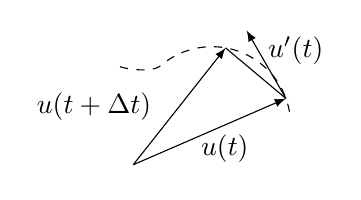
\begin{tikzpicture}
\draw[dashed]([shift={(10:1)}]1,0.5) arc (10:130:1) to [out=-135,in=180]++(-0.5,0);
\path(1,0.5)++(20:1)coordinate(kA);
\path(1,0.5)++(80:1)coordinate(kB);
\draw[-latex](0,0)--(kA)node[pos=0.6,below]{$\bM{u}(t)$};
\draw[-latex](0,0)--(kB)node[pos=0.3,above left]{$\bM{u}(t+\Delta t)$};
\draw(kA)--(kB);
\draw[-latex](kA)--++(120:1)node[pos=0.7,right]{$\bM{u}'(t)$};
\end{tikzpicture}
\caption{سمتی تفاعل کا تفرق}
\label{شکل_الاحصاء_سمتی_تفاعل_تفرق}
\end{figure}

کارتیسی نظام محدد استعمال کرتے ہوئے نقطہ \عددی{t}  پر \عددی{\bM{u}(t)} اس صورت قابل تفرق ہو گا جب اس نقطے پر درج ذیل تینوں تفرق موجود ہوں۔
\begin{align*}
u_m'(t)=\lim_{\Delta t\to 0}\frac{u_m(t+\Delta t)-u_m(t)}{\Delta t} \quad \quad (m=1,2,3)
\end{align*}
یوں سمتیہ تفاعل کا تفرق لینا اس کے تینوں ارکان کا علیحدہ علیحدہ تفرق لینے کے مترادف ہے یعنی:
\begin{align}
\bM{u}'(t)=u_1'(t)\bM{i}+u_2'(t)\bM{j}+u_3'(t)\bM{k}
\end{align}

تفرق کے جانی پہچانی اصولوں کے مطابقتی اصول سمتیہ تفاعل کے تفرق کے لئے بھی حاصل کیے جا سکتے ہیں مثلاً
\begin{align}
(c\bM{u})'=c\bM{u}' \,\, \text{(\RL{\عددی{c} مستقل ہے})},\quad \quad (\bM{u}+\bM{v})'=\bM{u}'+\bM{v}'
\end{align}
اور
\begin{align}
(\bM{u}\cdot \bM{v})'&=\bM{u}'\cdot \bM{v}+\bM{u}\cdot\bM{v}' \label{مساوات_سمتی_الاحصاء_ضرب_الف}\\
(\bM{u}\times \bM{v})'&=\bM{u}\times \bM{v}+\bM{u}\times \bM{v}'\label{مساوات_سمتی_الاحصاء_ضرب_ب}\\
\left(\frac{\bM{u}}{\bM{v}}\right)'&=\frac{\bM{v}\bM{u}-\bM{u}\bM{v}'}{\bM{v}^2}\label{مساوات_سمتی_الاحصاء_ضرب_پ}\\
(\bM{u}\bM{v}\bM{w})'&=(\bM{u}'\bM{v}\bM{w})+(\bM{u}\bM{v}'\bM{w})+(\bM{u}\bM{v}\bM{w}')\label{مساوات_سمتی_الاحصاء_ضرب_ت}
\end{align}
چونکہ سمتی ضرب غیر قابل تبادل ہے لہٰذا مساوات \حوالہ{مساوات_سمتی_الاحصاء_ضرب_ب} میں سمتیات کی ترتیب برقرار رکھنا لازم ہے۔ 

%================
\ابتدا{مثال}\شناخت{مثال_الاحصاء_مستقل_لمبائی_تفاعل_تفرق}\quad مستقل لمبائی کے تفاعل کا تفرق\\
اگر تفاعل \عددی{\bM{u}(t)} کی لمبائی مستقل ہو یعنی \عددی{\abs{\bM{u}(t)}=c} تب  \عددی{\abs{\bM{u}}^2=\bM{u}\cdot \bM{u}=c^2} ہو گا اور مساوات \حوالہ{مساوات_سمتی_الاحصاء_ضرب_الف} کی مدد سے  \عددی{(\bM{u}\cdot \bM{u})'=2\bM{u}\cdot \bM{u}'=0} حاصل ہو گا جس کے تحت مستقل لمبائی کے سمتی تفاعل کا تفرق یا صفر سمتیہ  ہو گا اور یا یہ \عددی{\bM{u}(t)} کے قائمہ الزاویہ ہو گا۔
\انتہا{مثال}
%========================

درج بالا گفتگو سے سمتی تفاعل کی جزوی تفرق کے اصول حاصل کرتے ہیں۔اگر کسی سمتی تفاعل \عددی{\bM{u}}
\begin{align*}
\bM{u}=u_1\bM{i}+u_2\bM{j}+u_3\bM{k}
\end{align*}
کے اجزاء \عددی{n} عدد متغیرات \عددی{t_1}، \نقطے، \عددی{t_n} کے ساتھ قابل تفرق ہوں تب \عددی{t_1} کے ساتھ \عددی{\bM{u}} کے جزوی تفرق کو
 \عددی{\tfrac{\partial \bM{u}}{\partial t_1}} سے ظاہر کیا جائے گا جو درج ذیل ہو گا۔
\begin{align*}
\frac{\partial \bM{u}}{\partial t_1}=\frac{\partial u_1}{\partial t_1}\bM{i}+\frac{\partial u_2}{\partial t_1}\bM{j}+\frac{\partial u_3}{\partial t_1}\bM{k}
\end{align*}
اسی طرح دیگر جزوی تفرقات لکھے جا سکتے ہیں مثلاً:
\begin{align*}
\frac{\partial^{\,2}\bM{u}}{\partial t_m \partial t_n}=\frac{\partial^{\,2} \bM{u}_1}{\partial t_m\partial t_n}\bM{i}+\frac{\partial^{\,2} \bM{u}_2}{\partial t_m\partial t_n}\bM{j}+\frac{\partial^{\,2} \bM{u}_3}{\partial t_m\partial t_n}\bM{k}
\end{align*}

%===============
\ابتدا{مثال}\quad جزوی تفرق\\
سمتی تفاعل \عددی{\bM{r}(t_1,t_2)=a\cos \omega t_1\bM{i}+a\sin\omega t_1\bM{j}+t_2\bM{k}} کے جزوی تفرق درج ذیل ہیں۔ 
\begin{align*}
\frac{\partial \bM{r}}{\partial t_1}=a\omega (-\sin \omega t_1\bM{i}+\cos \omega t_1\bM{j}),\quad \frac{\partial \bM{r}}{\partial t_2}=\bM{k}
\end{align*}
تفاعل \عددی{\bM{r}} ایسی نلکی سطح کو ظاہر کرتا ہے جس کا رداس \عددی{a} ہے  اور محور \عددی{z} محور ہے۔ 
\انتہا{مثال}
%=================================

\حصہء{سوالات}

%==================================
سوال \حوالہ{سوال_الاحصاء_برابر_سطح_الف} تا سوال \حوالہ{سوال_الاحصاء_برابر_سطح_ب} میں برابر سطح \عددی{f=c} کیا ہو گا جہاں \عددی{c} مستقل ہے۔

%===========================
\ابتدا{سوال}\شناخت{سوال_الاحصاء_برابر_سطح_الف}\quad
$f=x+y+z$\\
جواب:متوازی سطحیں
\انتہا{سوال}
%==============================
\ابتدا{سوال}\quad
$f=x^2+y^2+z^2$\\
جواب:ہم مرکز کرہ
\انتہا{سوال}
%==============================
\ابتدا{سوال}\quad
$f=x^2+y^2$\\
جواب:کارتیسی \عددی{z}  کے ہم محوری نلکی سطحیں
\انتہا{سوال}
%==============================
\ابتدا{سوال}\quad
$f=4x^2+5y^2$\\
جواب:کارتیسی \عددی{z}  کے ہم محوری نلکی ترخیم سطحیں
\انتہا{سوال}
%==============================
\ابتدا{سوال}\شناخت{سوال_الاحصاء_برابر_سطح_ب}\quad
$f=x^2+y^2-z$\\
جواب:قطع مکافی نما سطحیں
\انتہا{سوال}
%==============================
\عددی{xy} سطح پر سمتیہ \عددی{\bM{v}} سوال \حوالہ{سوال_الاحصاء_لمبائی_سمت_الف} تا سوال \حوالہ{سوال_الاحصاء_لمبائی_سمت_ب} میں دیا گیا ہے۔وہ سطح دریافت کریں جس پر \عددی{\bM{v}} کی لمبائی مستقل ہو۔وہ سطح دریافت کریں جس پر \عددی{\bM{v}}  کی یکساں سمت ہو۔ 
%===================

\ابتدا{سوال}\شناخت{سوال_الاحصاء_لمبائی_سمت_الف}\quad 
$\bM{v}=2x\bM{i}+3y\bM{j}$\\
جوابات:
$4x^2+9y^2=\text{مستقل},\,\, \tfrac{y}{x}=\text{مستقل}$
\انتہا{سوال}
%============================
\ابتدا{سوال}\quad 
$\bM{v}=x^2\bM{i}+\sqrt{y}\bM{j}$\\
جوابات:
$x^4+y=\text{مستقل},\,\, \tfrac{\sqrt{y}}{x^2}=\text{مستقل}$
\انتہا{سوال}
%============================
\ابتدا{سوال}\quad 
$\bM{v}=(x^2-y^2)\bM{i}+2xy\bM{j}$\\
جوابات:
$x^2+y^2=\text{مستقل},\,\, \tfrac{2xy}{x^2-y^2}=\text{مستقل}$
\انتہا{سوال}
%============================
\ابتدا{سوال}\شناخت{سوال_الاحصاء_لمبائی_سمت_ب}\quad 
$\bM{v}=(x+y)\bM{i}+(x-y)\bM{j}$\\
جوابات:
$x^2+y^2=\text{مستقل},\,\, \tfrac{x-y}{x+y}=\text{مستقل}$
\انتہا{سوال}
%============================
سوال \حوالہ{سوال_الاحصاء_تفرقات_الف} تا سوال \حوالہ{سوال_الاحصاء_تفرقات_ب} میں \عددی{\bM{u}} دیا گیا ہے۔آپ سے التماس ہے کہ \عددی{\bM{u}'} اور  \عددی{\bM{u}''} دریافت کریں۔

%========================
\ابتدا{سوال}\quad \شناخت{سوال_الاحصاء_تفرقات_الف}\quad
$\bM{a}+\bM{b}t^2$\\
جوابات:
$\bM{u}'=2\bM{b}t,\,\, \bM{u}''=2\bM{b}$
\انتہا{سوال}
%============================
\ابتدا{سوال}\quad
$t\bM{i}+(t^2+2)\bM{j}$\\
جوابات:
$\bM{u}'=\bM{i}+2t\bM{j},\,\, \bM{u}''=2\bM{j}$
\انتہا{سوال}
%============================
\ابتدا{سوال}\quad
$4\cos t\,\bM{i}+2\sin t\,\bM{j}$\\
جوابات:
$\bM{u}'=-4\sin t\,\bM{i}+2\cos t\,\bM{j},\,\, \bM{u}''=-4\cos t\,\bM{i}-2\sin t\,\bM{j}=-\bM{u}$
\انتہا{سوال}
%============================
\ابتدا{سوال}\quad
$4\cos t\,\bM{i}+2\sin t\,\bM{j}-3t\,\bM{k}$\\
جوابات:
$\bM{u}'=-4\sin t\,\bM{i}+2\cos t\,\bM{j}-3\,\bM{k},\,\, \bM{u}''=-4\cos t\,\bM{i}-2\sin t\,\bM{j}$
\انتہا{سوال}
%============================
\ابتدا{سوال}\quad
$t^2\bM{i}+2 \bM{j}+4t\bM{k}$\\
جوابات:
$\bM{u}'=2t\bM{i}+4\bM{k},\,\, \bM{u}''=2\bM{i}$
\انتہا{سوال}
%============================
\ابتدا{سوال}\quad
$\cos 2t\, \bM{i}-3\sin 2t \,\bM{j}+t^2\,\bM{k}$\\
جوابات:
$\bM{u}'=-2\sin 2t\,\bM{i}-6\cos 2t\,\bM{j}+2t\,\bM{k},\,\, \bM{u}''=-4\cos 2t\,\bM{i}+12\sin 2t\,\bM{j}+2\,\bM{k}$
\انتہا{سوال}
%============================
\ابتدا{سوال}\quad
$e^{t}\, \bM{i}-2e^{-3t} \,\bM{j}$\\
جوابات:
$\bM{u}'=e^t\,\bM{i}+6e^{-3t}\,\bM{j},\,\, \bM{u}''=e^t\,\bM{i}-18e^{-3t}\,\bM{j}$
\انتہا{سوال}
%============================
\ابتدا{سوال}\quad
$e^{-t}(\cos t\, \bM{i}-\sin t \,\bM{j})$\\
جوابات:
$\bM{u}'=e^{-t}[-(\cos t+\sin t)\,\bM{i}-(\cos t-\sin t)\,\bM{j}],\,\, \bM{u}''=e^{-t}(2\sin t \,\bM{i}+2\cos t \,\bM{j})$
\انتہا{سوال}
%============================
\ابتدا{سوال}\شناخت{سوال_الاحصاء_تفرقات_ب}\quad
$t^2(2\bM{i}-5\bM{j})$\\
جوابات:
$\bM{u}'=2t(2\bM{i}-5\bM{j}),\,\, \bM{u}''=2(2\bM{i}-5\bM{j})$
\انتہا{سوال}
%============================
سوال \حوالہ{سوال_الاحصاء_ضرب_تفرق_الف} تا سوال \حوالہ{سوال_الاحصاء_ضرب_تفرق_ب} میں \عددی{\bM{u}=t\bM{i}+t^3\bM{k}}،
 \عددی{\bM{v}=t^2\bM{j}+t\bM{k}} اور \عددی{\bM{w}=2\bM{i}+t\bM{j}-t^2\bM{k}} لیتے ہوئے حل کریں۔

%===============
\ابتدا{سوال}\شناخت{سوال_الاحصاء_ضرب_تفرق_الف}\quad
$(\bM{u}\cdot \bM{v})'$\\
جواب:\عددی{4t^3}
\انتہا{سوال}
%========================
\ابتدا{سوال}\quad
$(\bM{u}\times \bM{v})'$\\
جواب:
$-t^4\bM{i}-2t\bM{j}+3t^2\bM{k}$
\انتہا{سوال}
%========================
\ابتدا{سوال}\quad
$[\bM{u}\times (\bM{v}\times \bM{w})]'$\\
جواب:
$-8t^3\bM{i}-(7t^6+5t^4-6t^2)\bM{j}+4t\bM{k}$
\انتہا{سوال}
%========================
\ابتدا{سوال}\quad
$[(\bM{u}\times \bM{v})\times \bM{w}]'$\\
جواب:
$(6t^2-7t^6)\bM{j}+(4t-6t^5)\bM{k}$
\انتہا{سوال}
%========================
\ابتدا{سوال}\شناخت{سوال_الاحصاء_ضرب_تفرق_ب}\quad
$[(\bM{u}\times \bM{v})\cdot\bM{w}]'$\\
جواب:
$-15t^4-3t^2$
\انتہا{سوال}
%========================
سوال \حوالہ{سوال_الاحصاء_جزوی_الف} تا سوال \حوالہ{سوال_الاحصاء_جزوی_ب} میں دیے گئے سمتی تفاعل \عددی{\bM{u}} کا  \عددی{x}، \عددی{y}  اور \عددی{z} کے ساتھ جزوی تفرق دریافت کریں۔

%===============
\ابتدا{سوال}\شناخت{سوال_الاحصاء_جزوی_الف}\quad
$x\bM{i}+3y\bM{k}$\\
جوابات:
$\bM{i},\,\, 3\bM{k},\,\, 0$
\انتہا{سوال}
%======================
\ابتدا{سوال}\quad
$(x^2-y^2)\bM{i}+2xy\bM{j}$\\
جوابات:
$2x\bM{i}+2y\bM{j},\,\, -2y\bM{i}+2x\bM{j},\,\, 0$
\انتہا{سوال}
%======================
\ابتدا{سوال}\quad
$x^2\bM{i}-3y^2\bM{j}+2z^2\bM{k}$\\
جوابات:
$2x\bM{i},\,\, -6y\bM{j},\,\,4z\bM{k}$
\انتہا{سوال}
%======================
\ابتدا{سوال}\quad
$xy\bM{i}+yz\bM{j}+zx\bM{k}$\\
جوابات:
$y\bM{i}+z\bM{k},\,\, x\bM{i}+z\bM{j},\,\,y\bM{j}+x\bM{k}$
\انتہا{سوال}
%======================
\ابتدا{سوال}\quad
$(x+y)\bM{i}+(y+z)\bM{j}+(z+x)\bM{k}$\\
جوابات:
$\bM{i}+\bM{k},\,\, \bM{i}+\bM{j},\,\,\bM{j}+\bM{k}$
\انتہا{سوال}
%======================
\ابتدا{سوال}\شناخت{سوال_الاحصاء_جزوی_ب}\quad
$x^2y\bM{i}+y^2z\bM{j}+z^2x\bM{k}$\\
جوابات:
$2xy\bM{i}+z^2\bM{k},\,\, x^2\bM{i}+2yz\bM{j},\,\,y^2\bM{j}+2xz\bM{k}$
\انتہا{سوال}
%======================
\ابتدا{سوال}
\عددی{(\bM{u}\cdot \bM{v})''} اور \عددی{(\bM{u}\times \bM{v})''} کے لئے مساوات \حوالہ{مساوات_سمتی_الاحصاء_ضرب_الف} اور مساوات \حوالہ{مساوات_سمتی_الاحصاء_ضرب_ب} کی طرز کے کلیات دریافت کریں۔

جوابات:
$(\bM{u}\cdot \bM{v})''=\bM{u}''\cdot \bM{v}+2\bM{u}'\cdot \bM{v}'+\bM{u}\cdot \bM{v}'' $, \\  $(\bM{u}\times \bM{v})''=\bM{u}''\times \bM{v}+2\bM{u}'\times \bM{v}'+\bM{u}\times \bM{v}''$
\انتہا{سوال}
%===========================
\ابتدا{سوال}
ثابت کریں کہ
$\left(\tfrac{\bM{u}}{\abs{\bM{u}}}\right)'=\tfrac{\bM{u}'(\bM{u}\cdot \bM{u})-\bM{u}(\bM{u}\cdot \bM{u}')}{(\bM{u}\cdot \bM{u})^{\tfrac{3}{2}}}$\\
جواب:
$\left(\tfrac{\bM{u}}{\abs{\bM{u}}}\right)'=\left(\tfrac{\bM{u}}{\sqrt{\bM{u}\cdot \bM{u}}}\right)'$
 لکھتے ہوئے  مساوات \حوالہ{مساوات_سمتی_الاحصاء_ضرب_پ} کا استعمال کریں۔
\انتہا{سوال}
%===========================

\حصہ{منحنی}\شناخت{حصہ_الاحصاء_منحنی}
کارتیسی نظام میں منحنی \عددی{C} کو  درج ذیل سمتی تفاعل سے ظاہر کیا جا سکتا ہے (شکل \حوالہ{شکل_الاحصاء_منحنی_مقدار_معلوم}-الف)۔
\begin{align}\label{مساوات_الاحصاء_منحنی_مقدار_معلوم_الف}
\bM{r}(t)=x(t)\bM{i}+y(t)\bM{j}+z(t)\bM{k}
\end{align} 
آزاد حقیقی متغیرہ \عددی{t} کی ہر قیمت \عددی{t_0} کا \عددی{C} پر مطابقتی نقطہ پایا جاتا ہے جس  کے محدد \عددی{x(t_0)}،\عددی{y(t_0)} اور \عددی{z(t_0)} 
  تعین گر سمتیہ \عددی{\bM{r}(t_0)} دیتا ہے۔
\begin{figure}
\centering
\begin{subfigure}{0.5\textwidth}
\centering
\begin{tikzpicture}
%axis
\draw(0,0)--++(-0.25,-0.5)node[left]{$x$};
\draw(0,0)--++(1,0)node[below]{$y$};
\draw(0,0)--++(0,0.5)node[left]{$z$};
%curve
\draw(0.3,1) to [out=30,in=150]++(1.5,0.5)coordinate(kA) to [out=-30,in=-90]++(1,0.5)node[left]{$C$};
\draw[-latex](0,0)node[ocirc]{}--(kA)node[ocirc]{}node[pos=0.7,below right]{$\bM{r}(t)$};
\end{tikzpicture}
\caption*{(الف) منحنی مقدار معلوم}
\end{subfigure}%
\begin{subfigure}{0.5\textwidth}
\centering
\begin{tikzpicture}
%axis
\draw(0,0)--++(-0.25,-0.5)node[left]{$x$};
\draw(0,0)--++(1,0)node[below]{$y$};
\draw(0,0)--++(0,0.5)node[left]{$z$};
%straight line
\draw(-0.3,1)--++(2.5,0.5)node[right]{$L$}coordinate[pos=0.3](kB)coordinate[pos=0.7](kA);
\draw[-latex](0,0)node[ocirc]{}--(kA)node[ocirc]{}node[above]{$A$}node[pos=0.7,right]{$\bM{a}$};
\draw[-latex](kA)node[ocirc]{}--(kB)node[ocirc]{}node[pos=0.7,above]{$\bM{b}$};
\end{tikzpicture}
\caption*{(ب) سیدھی لکیر کا مقدار معلوم خط}
\end{subfigure}%
\caption{سیدھی لکیر اور منحنی کے مقدار معلوم خطوط۔}
\label{شکل_الاحصاء_منحنی_مقدار_معلوم}
\end{figure}
مساوات \حوالہ{مساوات_الاحصاء_منحنی_مقدار_معلوم_الف}  کو \عددی{C} کی \اصطلاح{منحنی مقدار معلوم}\فرہنگ{منحنی!مقدار معلوم}\فرہنگ{مقدار معلوم!منحنی}\حاشیہب{parametric representation}\فرہنگ{parametric!representation} کہتے ہیں جبکہ \عددی{t} کو \اصطلاح{مقدار معلوم} کہتے ہیں۔ منحنی مقدار معلوم کی طرز پر منحنی کا اظہار نہایت عمدہ ثابت ہوتا ہے۔

فضا میں منحنی ظاہر کرنے کے دیگر طریقے 
\begin{align}\label{مساوات_الاحصاء_منحنی_مقدار_معلوم_ب}
y=f(x),\quad z=g(x)
\end{align} 
اور
\begin{align}\label{مساوات_الاحصاء_منحنی_مقدار_معلوم_پ}
F(x,y,z)=0,\quad G(x,y,z)=0
\end{align}
ہیں۔مساوات \حوالہ{مساوات_الاحصاء_منحنی_مقدار_معلوم_ب} میں \عددی{x=t} پر کرتے ہوئے اس کو مساوات \حوالہ{مساوات_الاحصاء_منحنی_مقدار_معلوم_الف} کی طرح لکھ سکتے ہیں یعنی:
\begin{align*}
\bM{r}(t)=t\bM{i}+f(t)\bM{j}+g(t)\bM{k}
\end{align*}
مساوات \حوالہ{مساوات_الاحصاء_منحنی_مقدار_معلوم_پ} میں دو سطحوں کے مساوات دیے گئے ہیں جن کا ملاپ منحنی دیتا ہے۔

\اصطلاح{مستوی منحنی}\فرہنگ{مستوی!منحنی}\فرہنگ{منحنی!مستوی}\حاشیہب{plane curve}\فرہنگ{plane curve} سے مراد ایسی منحنی ہے جو فضا میں کسی سطح مستوی پر پائی جاتی ہو۔غیر مستوی منحنی کو \اصطلاح{خم دار منحنی}\فرہنگ{خم دار منحنی}\فرہنگ{منحنی!خم دار}\حاشیہب{twisted curve}\فرہنگ{twisted curve} کہتے ہیں۔

%=======================
\ابتدا{مثال}\quad سیدھا خط\\
کسی بھی سیدھی لکیر \عددی{L} کو درج ذیل لکھا جا سکتا ہے جہاں \عددی{\bM{a}} اور \عددی{\bM{b}} مستقل سمتیات ہیں (شکل \حوالہ{شکل_الاحصاء_منحنی_مقدار_معلوم}-ب)۔
\begin{align}
\bM{r}(t)=\bM{a}+t\bM{b}=(a_1+tb_1)\bM{i}+(a_2+tb_2)\bM{j}+(a_3+tb_3)\bM{k}
\end{align}
\عددی{L} نقطہ \عددی{A} سے گزرتی ہے جس کا تعین گر سمتیہ \عددی{\bM{a}} ہے جبکہ \عددی{\bM{b}} کے رخ \عددی{L}  ہو گا۔اگر \عددی{\bM{b}} اکائی سمتیہ ہو تب اس کے ارکان \اصطلاح{کوسائن رخ}\فرہنگ{کوسائن رخ}\حاشیہب{direction cosines}\فرہنگ{direction cosines} ہوں گے اور \عددی{L} پر کسی بھی نقطے کا \عددی{A} سے فاصلہ  \عددی{\abs{t}} ہو گا۔
\انتہا{مثال}
%==========================
\ابتدا{مثال}\quad ترخیم، دائرہ\\
درج ذیل سمتی تفاعل \عددی{xy} سطح میں ترخیم کو ظاہر کرتا ہے جس کا مرکز کارتیسی نظام کے مبدا  اور صدر محور \عددی{x} اور \عددی{y} محور پر ہیں۔  
\begin{align}\label{مساوات_الاحصاء_ترخیم_الف}
\bM{r}(t)=a\cos t \bM{i}+b\sin t\bM{j}
\end{align}
\عددی{x=a\cos t} اور \عددی{y=b\sin t} لیتے ہوئے \عددی{\cos^2 t+\sin^2 t=1} کے استعمال سے 
\begin{align}
\frac{x^2}{a^2}+\frac{y^2}{b^2}=1, \quad z=0
\end{align}
ملتا ہے جو ترخیم کی مساوات ہے۔اگر \عددی{a=b} ہو تب مساوات \حوالہ{مساوات_الاحصاء_ترخیم_الف} رداس \عددی{a} کی دائرے کی مساوات ہو گی۔
\انتہا{مثال}
%==============================
\ابتدا{سوال}\quad مبدا سے ہٹ کر دائرہ\\
\عددی{xy} سطح میں رداس \عددی{r} کا  ایسا دائرہ جس کا مرکز نقطہ \عددی{(x_0,y_0)} پر ہو کی مساوات درج ذیل ہے۔
\begin{align*}
\frac{(x-x_0)^2}{r^2}+\frac{(y-y_0)^2}{r^2}=1
\end{align*} 
\عددی{\tfrac{x-x_0}{r}=\cos t} اور \عددی{\tfrac{y-y_0}{r}=\sin t} لیتے ہوئے \عددی{x=x_0+r\cos t} اور \عددی{y=y_0+r\sin t} لکھا جا سکتا ہے لہٰذا اس دائرے کی مقدار معلوم مساوات درج ذیل ہو گی۔
\begin{align}
\bM{r}(t)=(x_0+r\cos t)\bM{i}+(y_0+r\sin t)\bM{j}
\end{align} 
\انتہا{سوال}
%=================================
\ابتدا{سوال}\شناخت{مثال_الاحصاء_پیچ_دار}\quad پیچ دار لچھا\\
\اصطلاح{پیچ دار لچھے}\فرہنگ{پیچ دار لچھا}\حاشیہب{circular helix}\فرہنگ{helix!circular} کو
\begin{align}\label{مساوات_الاحصاء_پیچ_دار_لچھا}
\bM{r}(t)=a\cos t\bM{i}+a\sin t\bM{j}+ct\bM{k}\quad \quad (c \ne 0)
\end{align}
ظاہر کرتا ہے۔اس \اصطلاح{خم دار منحنی} کو \عددی{c>0} (دایاں ہاتھ پیچ دار لچھا) اور \عددی{c<0} (بایاں ہاتھ پیچ دار لچھا) کے لئے  شکل \حوالہ{شکل_الاحصاء_پیچدار} میں دکھایا گیا ہے۔
\begin{figure}
\centering
\begin{subfigure}{0.5\textwidth}
\centering
\begin{tikzpicture}[x={(-0.5cm,-0.5cm)},y={(1cm,0cm)},z={(0cm,1cm)}]
\pgfmathsetmacro{\ang}{30}
\pgfmathsetmacro{\h}{1.5}
\pgfmathsetmacro{\c}{\h/450}
%axis
\draw(0.075,0,0)--(1.5,0,0)node[left]{$x$};
\draw(0,0.075,0)--(0,1.5,0)node[below]{$y$};
\draw[dashed](0,0,0)--(0,0,\h);
\draw(0,0,\h)--++(0,0,1)node[left]{$z$};
%curve
\draw[domain=0:90+\ang,smooth,variable=\t] plot ({cos(\t)},{sin(\t)},{\c*\t});
\draw[dashed,domain=90+\ang:270+\ang,smooth,variable=\t] plot ({cos(\t)},{sin(\t)},{\c*\t});
\draw[domain=270+\ang:450,smooth,variable=\t] plot ({cos(\t)},{sin(\t)},{\c*\t});
%arrow
\draw[-stealth] ({cos(80)},{sin(80)},{\c*80})--({cos(82)},{sin(82)},{\c*82});
%cylinder
\draw[domain=-90+\ang:90+\ang,smooth,variable=\t] plot ({cos(\t)},{sin(\t)},{0})coordinate(kA);
\draw(kA)--++(0,0,\h);
\draw({cos(-90+\ang)},{sin(-90+\ang)},0)--++(0,0,\h);
\draw[domain=0:360,smooth,variable=\t] plot ({cos(\t)},{sin(\t)},{\h})coordinate(kA);
%nodes
\draw[domain=-130:150,smooth,variable=\t] plot ({0.075*cos(\t)},{0.075*sin(\t)},{\h});
\path (1,0,0)node[ocirc]{};
\path[domain=270+\ang:450,smooth,variable=\t] plot ({cos(\t)},{sin(\t)},{\c*\t})node[ocirc]{};
\draw[domain=-130:150,smooth,variable=\t] plot ({0.075*cos(\t)},{0.075*sin(\t)},{0});
\end{tikzpicture}
\caption*{(الف) دایاں ہاتھ پیچ دار لچھا}
\end{subfigure}%
\begin{subfigure}{0.5\textwidth}
\centering
\begin{tikzpicture}[x={(-0.5cm,-0.5cm)},y={(1cm,0cm)},z={(0cm,1cm)}]
\pgfmathsetmacro{\ang}{30}
\pgfmathsetmacro{\h}{-1.5}
\pgfmathsetmacro{\c}{\h/450}
%axis
\draw(0.075,0,0)--(3,0,0)node[left]{$x$};
\draw(0,0.075,0)--(0,2,0)node[below]{$y$};
\draw(0,0,0)--(0,0,1)node[left]{$z$};
%curve
\draw[domain=0:90+\ang,smooth,variable=\t] plot ({cos(\t)},{sin(\t)},{\c*\t});
\draw[dashed,domain=90+\ang:270+\ang,smooth,variable=\t] plot ({cos(\t)},{sin(\t)},{\c*\t});
\draw[domain=270+\ang:450,smooth,variable=\t] plot ({cos(\t)},{sin(\t)},{\c*\t});
%arrow
\draw[-stealth] ({cos(80)},{sin(80)},{\c*80})--({cos(82)},{sin(82)},{\c*82});
%cylinder
\draw[domain=-90+\ang:90+\ang,smooth,variable=\t] plot ({cos(\t)},{sin(\t)},{\h})coordinate(kA);
\draw(kA)--++(0,0,-\h);
\draw({cos(-90+\ang)},{sin(-90+\ang)},0)--++(0,0,\h);
\draw[domain=0:360,smooth,variable=\t] plot ({cos(\t)},{sin(\t)},{0})coordinate(kA);
%nodes
\path (1,0,0)node[ocirc]{};
\path[domain=270+\ang:450,smooth,variable=\t] plot ({cos(\t)},{sin(\t)},{\c*\t})node[ocirc]{};
\draw[domain=-130:150,smooth,variable=\t] plot ({0.075*cos(\t)},{0.075*sin(\t)},{0});
\end{tikzpicture}
\caption*{(ب) بایاں ہاتھ پیچ دار لچھا}
\end{subfigure}%
\caption{پیچ دار لچھے (مثال \حوالہ{مثال_الاحصاء_پیچ_دار})۔}
\label{شکل_الاحصاء_پیچدار}
\end{figure}
\انتہا{سوال}
%====================================

منحنی کے کچھ حصے کو عموماً \اصطلاح{قوس}\فرہنگ{قوس}\حاشیہب{arc}\فرہنگ{arc} کہتے ہیں۔اس کتاب میں ہم عموماً قوس کو بھی منحنی کہیں گے۔
 
ہم قطع منحنی اپنی آپ کو قطع کرتی ہے۔ نقطہ قطع کو منحنی کا \اصطلاح{متعدد نقطہ}\فرہنگ{متعدد نقطہ}\حاشیہب{multiple point}\فرہنگ{multiple point} کہتے ہیں (شکل \حوالہ{شکل_الاحصاء_دوہرا_نقطہ})۔ ایسی منحنی جس کے متعدد نقطے نہ پائے جاتے ہوں \اصطلاح{سادہ منحنی}\فرہنگ{سادہ منحنی}\فرہنگ{منحنی!سادہ}\حاشیہب{simple curve}\فرہنگ{curve!simple} کہلاتی ہے۔
\begin{figure}
\centering
\begin{subfigure}{0.5\textwidth}
\centering
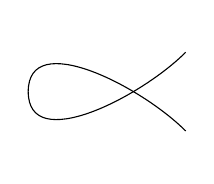
\begin{tikzpicture}
\draw(0,0) to [out=90,in=135]++(2,-0.5);
\draw(0,0) to [out=-90,in=-135]++(2,0.5);
\end{tikzpicture}
\end{subfigure}%
\begin{subfigure}{0.5\textwidth}
\centering
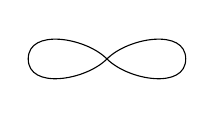
\begin{tikzpicture}
\draw(0,0) to [out=90,in=135]++(1,0) to [out=-45,in=-90]++(1,0);
\draw(0,0) to [out=-90,in=-135]++(1,0) to [out=45,in=90]++(1,0);
\end{tikzpicture}
\end{subfigure}%
\caption{دوہرا نقطوں والے منحنی}
\label{شکل_الاحصاء_دوہرا_نقطہ}
\end{figure}

%===============
\ابتدا{مثال}\quad سادہ اور غیر سادہ منحنی\\
ترخیم اور پیچ دار لچھے سادہ ترخیم کی مثالیں ہیں۔درج ذیل \عددی{t=1} اور \عددی{t=-1} پر مبدا سے دو مرتبہ گزرتی ہے لہٰذا یہ غیر سادہ منحنی کی مثال ہے۔
\begin{align*}
\bM{r}(t)=(t^2-1)\bM{i}+(t^3-1)\bM{j}
\end{align*}
\انتہا{مثال}
%=========================

آخر میں بتاتا چلوں کہ کسی بھی منحنی \عددی{C} کو کئی سمتی تفاعل سے ظاہر کیا جا سکتا ہے مثلاً اگر \عددی{C} کو مساوات \حوالہ{مساوات_الاحصاء_منحنی_مقدار_معلوم_الف} ظاہر کرے تب ہم \عددی{t=h(t^*)} لیتے ہوئے، جہاں مساوات \حوالہ{مساوات_الاحصاء_منحنی_مقدار_معلوم_الف} میں استعمال \عددی{t} کی تمام قیمتوں کے لئے  \عددی{h(t^*)} بھی پائے جاتے ہوں،  \عددی{C} کو نئی سمتی تفاعل \عددی{\tilde{\bM{r}}(t^*)=\bM{r}[h(t^*)]} سے ظاہر کر سکتے ہیں۔

%============
\ابتدا{مثال}\quad مقدار معلوم کی تبدیلی\\
\عددی{xy} سطح میں قطع مکافی \عددی{y=x^2} کو درج ذیل سمتیہ تفاعل ظاہر کرتی ہے۔
\begin{align}
\bM{r}=t\bM{i}+t^2\bM{j}\quad \quad (-\infty < t < \infty)
\end{align}
ہم \عددی{t=-2t^*} لیتے ہوئے اس قطع مکافی کو درج ذیل سمتی تفاعل سے ظاہر کر سکتے ہیں۔
\begin{align*}
\tilde{\bM{r}}(t^*)=\bM{r}(-2t^*)=-2t^*\bM{i}+4t^{*2}\bM{j}
\end{align*}
اگر ہم \عددی{t=t^{*2}} لیں تب ہمیں درج ذیل نیا سمتی تفاعل ملتا ہے
\begin{align*}
\tilde{\bM{r}}(t^*)=t^{*2}\bM{i}+t^{*4}\bM{j}
\end{align*} 
لیکن \عددی{t^{*2}>0} کی بنا یہ تفاعل قطع مکافی کو صرف ربع اول میں ظاہر کرتا ہے۔
\انتہا{مثال}
%======================

\حصہء{سوالات}
سوال \حوالہ{سوال_الاحصاء_مقدار_معلوم_خط_الف} تا سوال \حوالہ{سوال_الاحصاء_مقدار_معلوم_خط_ب} میں نقطہ \عددی{A} سے گزرتی ہوئی سمتیہ \عددی{\bM{b}} کے رخ سیدھی لکیر کی مقدار معلوم مساوات دریافت کریں۔

%================
\ابتدا{سوال}\شناخت{سوال_الاحصاء_مقدار_معلوم_خط_الف}\quad 
$A:(0,0,0),\quad \bM{b}=\bM{i}-\bM{j}$\\
جواب:
$\bM{r}=t\bM{i}-t\bM{j}$
\انتہا{سوال}
%====================
\ابتدا{سوال}\quad 
$A:(2,-3,1),\quad \bM{b}=\bM{i}+2\bM{j}$\\
جواب:
$\bM{r}=(t+2)\bM{i}+(2t-3)\bM{j}+\bM{k}$
\انتہا{سوال}
%====================
\ابتدا{سوال}\quad 
$A:(2,0,-3),\quad \bM{b}=-\bM{j}+3\bM{k}$\\
جواب:
$\bM{r}=2\bM{i}-t\bM{j}+3(t-1)\bM{k}$
\انتہا{سوال}
%====================
\ابتدا{سوال}\شناخت{سوال_الاحصاء_مقدار_معلوم_خط_ب}\quad 
$A:(-3,2,6),\quad \bM{b}=5\bM{i}+3\bM{j}-7\bM{k}$\\
جواب:
$\bM{r}=(5t-3)\bM{i}+(3t+2)\bM{j}+(6-7t)\bM{k}$
\انتہا{سوال}
%====================
سوال \حوالہ{سوال_الاحصاء_مقدار_معلوم_سیدھی_لکیر_الف} تا سوال \حوالہ{سوال_الاحصاء_مقدار_معلوم_سیدھی_لکیر_ب} میں نقطہ \عددی{A} اور نقطہ \عددی{B} سے گزرتی ہوئی سیدھی لکیر کی مقدار معلوم مساوات دریافت کریں۔

%=========
\ابتدا{سوال}\شناخت{سوال_الاحصاء_مقدار_معلوم_سیدھی_لکیر_الف} \quad
$A:(0,0,0),\quad B:(1,1,1)$\\
جواب:
$\bM{r}=t\bM{i}+t\bM{j}+t\bM{k}$
\انتہا{سوال}
%======================
\ابتدا{سوال}\quad
$A:(-3,7,-5),\quad B:(2,0,3)$\\
جواب:
$\bM{r}=(5t-3)\bM{i}+7(1-t)\bM{j}+(8t-5)\bM{k}$
\انتہا{سوال}
%======================
\ابتدا{سوال}\quad
$A:(1,2,-3),\quad B:(7,2,-3)$\\
جواب:
$\bM{r}=(6t+1)\bM{i}+2\bM{j}-3\bM{k}$
\انتہا{سوال}
%======================
\ابتدا{سوال}\شناخت{سوال_الاحصاء_مقدار_معلوم_سیدھی_لکیر_ب}\quad
$A:(3,2,0),\quad B:(0,0,0)$\\
جواب:
$\bM{r}=3(1-t)\bM{i}+2(1-t)\bM{j}$
 جس میں \عددی{t^*=1-t} چنتے ہوئے 
$\tilde{\bM{r}}=3t^*\bM{i}+2t^*\bM{j}$
 بھی لکھا جا سکتا ہے۔
\انتہا{سوال}
%======================

سوال \حوالہ{سوال_الاحصاء_مقدار_معلوم_درکار_الف} تا سوال \حوالہ{سوال_الاحصاء_مقدار_معلوم_درکار_ب} میں دیے سیدھی لکیر کی مقدار معلوم مساوات دریافت کریں۔

%==============
\ابتدا{سوال}\شناخت{سوال_الاحصاء_مقدار_معلوم_درکار_الف}\quad
$y=x,\quad z=0$\\
جواب:
$\bM{r}=t\bM{i}+t\bM{j}$
\انتہا{سوال}
%=====================
\ابتدا{سوال}\quad
$y=-3x,\quad z=2x$\\
جواب:
$\bM{r}=t\bM{i}-3t\bM{j}+2t\bM{k}$
\انتہا{سوال}
%=====================
\ابتدا{سوال}\quad
$2y=5x,\quad z=x-3y$\\
جواب:
$\bM{r}=t\bM{i}+\tfrac{5}{2}\bM{j}-\tfrac{13}{2}\bM{k}$ \quad 
یا \quad 
$\bM{r}=2t\bM{i}+5t\bM{j}-13t\bM{k}$\quad 
جہاں \عددی{t^*} کی جگہ \عددی{t} ہی لکھا گیا ہے۔
\انتہا{سوال}
%=====================
\ابتدا{سوال}\quad
$4x-y+z=3,\quad -3x+2y+3z=19$\\
جواب:\عددی{y} اور \عددی{z} حاصل کرتے ہوئے  \quad
$\bM{r}=t\bM{i}+(3t+2)\bM{j}+(5-t)\bM{k}$
\انتہا{سوال}
%=====================
\ابتدا{سوال}\شناخت{سوال_الاحصاء_مقدار_معلوم_درکار_ب}\quad
$x-y=2,\quad 2x+z=3$\\
جواب:
$\bM{r}=t\bM{i}+(t-2)\bM{j}+(3-2t)\bM{k}$
\انتہا{سوال}
%=====================
سوال \حوالہ{سوال_الاحصاء_عمومی_مقدار_معلوم_الف} تا سوال \حوالہ{سوال_الاحصاء_عمومی_مقدار_معلوم_ب} میں دیے خطوط کی مقدار معلوم مساوات دریافت کریں۔

%================
\ابتدا{سوال}\شناخت{سوال_الاحصاء_عمومی_مقدار_معلوم_الف} \quad
$x^2+y^2=1,\quad z=0$\\
جواب:
$\bM{r}=\cos t\bM{i}+\sin t\bM{j}$
\انتہا{سوال}
%===================
\ابتدا{سوال}\quad
$y=x^3,\quad z=0$\\
جواب:
$\bM{r}=t\bM{i}+t^3\bM{j}$
\انتہا{سوال}
%===================
\ابتدا{سوال}\quad
$y=2x^3,\quad z=-3x^2$\\
جواب:
$\bM{r}=t\bM{i}+2t^3\bM{j}-3t^2\bM{k}$
\انتہا{سوال}
%===================
\ابتدا{سوال}\quad
$x^2+y^2-4x+6y=-9,\quad z=0$\\
جواب: نقطہ \عددی{(2,-3)} پر رداس \عددی{2} کا دائرہ \quad
$\bM{r}=(2+2\cos t)\bM{i}+(-3+2\sin t)\bM{j}$
\انتہا{سوال}
%===================
\ابتدا{سوال}\quad
$4(x+1)^2+y^2=4,\quad z=0$\\
جواب:
$\bM{r}=(-1+2\cos t)\bM{i}+2\sin t\bM{j}$
\انتہا{سوال}
%===================
\ابتدا{سوال}\quad
$x=-5y^2,\quad z=2y^3$\\
جواب:
$\bM{r}=-5t^2\bM{i}+t\bM{j}+2t^3\bM{k}$
\انتہا{سوال}
%=====================
\ابتدا{سوال}\quad
$y=\sqrt{x},\quad z=y-2,\quad $\\
جواب:
$\bM{r}=t^2\bM{i}+t\bM{j}+(t-2)\bM{k}$
\انتہا{سوال}
%=====================
\ابتدا{سوال}
\عددی{xy} سطح میں درج ذیل ترخیم کی مقدار معلوم مساوات لکھیں۔
\begin{align*}
\frac{(x-x_0)^2}{a^2}+\frac{(y-y_0)^2}{b^2}=1
\end{align*}
جواب:
$\bM{r}=(x_0+a\cos t)\bM{i}+(y_0+b\sin t)\bM{j}$
\انتہا{سوال}
%====================
\ابتدا{سوال}\شناخت{سوال_الاحصاء_عمومی_مقدار_معلوم_ب}\quad
$x^2+y^2=4,\quad z=e^{-x}$\\
جواب:
$\bM{r}=2\cos t\bM{i}+2\sin t\bM{j}+e^{-t}\bM{k}$
\انتہا{سوال}
%===================
\ابتدا{سوال}
پیچ دار لچھے (مساوات \حوالہ{مساوات_الاحصاء_پیچ_دار_لچھا}) کا \عددی{xy}، \عددی{xz} اور \عددی{yz} سطحوں پر عمودی سایہ کیا ہو گا؟

جوابات:\عددی{xy} میں دائرہ، \عددی{xz} میں کوسائن موج اور \عددی{yz} میں سائن موج
\انتہا{سوال}
%====================

\حصہ{لمبائی قوس}\شناخت{حصہ_الاحصاء_لمبائی_قوس}
سادہ منحنی \عددی{C} کی لمبائی کی تعریف پیش کرتے ہیں۔ہم \عددی{C} (شکل \حوالہ{شکل_الاحصاء_لمبائی_قوس}-الف) کے دونوں سروں کے مابین متواتر (اختیاری) نقطوں کو \عددی{n} عدد (نقطہ دار) خط مستقیم سے یوں جوڑتے ہیں کہ \عددی{n \to \infty} کی صورت میں لمبی ترین خط مستقیم کی لمبائی صفر کے قریب تر ہو گی۔تمام خط مستقیم کی لمبائیوں (جنہیں مسئلہ فیثاغورث سے حاصل کیا جا سکتا ہے) کا مجموعہ لیتے ہیں۔اگر \عددی{n} کی بتدریج بڑھتی تعداد  \عددی{n_1}، \عددی{n_2}، \نقطے لیتے ہوئے مطابقتی خط مستقیم کی لمبائیوں کے مجموعے کی ترتیب  \عددی{l_1}، \عددی{l_2}،\نقطے مرکوز ہو جس کی حد \عددی{l} ہو تب ہم کہتے ہیں کہ \عددی{C}  \اصطلاح{قابل تصحیح}\فرہنگ{قابل تصحیح}\حاشیہب{rectifiable}\فرہنگ{rectifiable} ہے اور \عددی{l} کو \عددی{C} کی \اصطلاح{لمبائی}\فرہنگ{لمبائی!منحنی}\حاشیہب{length}\فرہنگ{length} کہتے ہیں۔ 

اگر \عددی{C} از خود سادہ منحنی نہ ہو لیکن یہ محدود تعداد کے قابل تصحیح سادہ منحنیات پر مشتمل ہو تب \عددی{C} کی \اصطلاح{لمبائی} سے مراد ان تمام منحنیات کی لمبائیوں کا مجموعہ ہو گا۔ 
\begin{figure}
\centering
\begin{subfigure}{0.5\textwidth}
\centering
\begin{tikzpicture}
\draw (1,0) to [out=150,in=-90] (0,1) to [out=90,in=180] (-0.5,2) to [out=0,in=135] (1.5,1.5) to [out=-45,in=170] (3.2,0);
\draw[dashed](1,0)node[ocirc,solid]{}--(0,1)node[ocirc,solid]{}--(-0.5,2)node[ocirc,solid]{}--(1.5,1.5)node[ocirc,solid]{}--(3.2,0)node[ocirc,solid]{};
\end{tikzpicture}
\caption*{(الف) لمبائی کی تعریف۔}
\end{subfigure}%
\begin{subfigure}{0.5\textwidth}
\centering
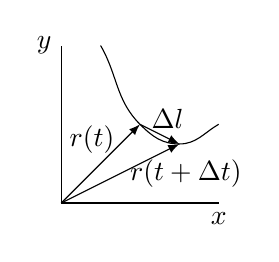
\begin{tikzpicture}
%axis
\draw(0,0)--(2,0)node[below]{$x$};
\draw(0,0)--(0,2)node[left]{$y$};
%
\draw(0.5,2) to [out=-60,in=135] (1,1) to [out=-45,in=180] (1.5,0.75) to [out=0,in=-150] (2,1);
\draw[-latex] (0,0) --(1,1)node[pos=0.8,left]{$\bM{r}(t)$};
\draw[-latex] (0,0) --(1.5,0.75)node[pos=0.5,right]{$\bM{r}(t+\Delta t)$};
\draw[-latex] (1,1)--(1.5,0.75)node[pos=0.7,above]{$\Delta \bM{l}$};
\end{tikzpicture}
\caption*{(ب) استمراری قابل تفرق تفاعل کی لمبائی۔}
\end{subfigure}%
\caption{لمبائی قوس}
\label{شکل_الاحصاء_لمبائی_قوس}
\end{figure}
%

اگر \عددی{C} کو استمراری\حاشیہد{استمراری قابل تفرق کا مطلب ہے کہ اس کا تفرق موجود ہے اور یہ تفرق استمراری ہے۔اسی طرح دوہرا استمراری قابل تفرق کا مطلب ہے کہ اس کا دوہرا تفرق موجود ہے اور یہ دوہرا تفرق استمراری ہے، وغیرہ وغیرہ}\شناخت{حاشیہ_الاحصاء_استمراری_قابل_تفرق} قابل تفرق سمتی تفاعل
\begin{align}
\bM{r}=\bM{r}(t) \quad \quad (a\le t\le b)
\end{align}
سے ظاہر کرنا ممکن ہو تب \عددی{\Delta \bM{l}=\bM{r}(t)-\bM{r}(t+\Delta t)=\Delta \bM{r}} ہو گا (شکل \حوالہ{شکل_الاحصاء_لمبائی_قوس}-ب)  جس کو \عددی{\Delta t} سے تقسیم کرتے ہوئے 
$\tfrac{\Delta \bM{l}}{\Delta t}=\tfrac{\Delta \bM{r}}{\Delta t}$
لکھا جا سکتا ہے۔ یوں \عددی{\Delta t \to 0} کی صورت میں درج ہو گا۔
\begin{align*}
\frac{\dif \bM{l}}{\dif t}=\frac{\dif \bM{r}}{\dif t}=\dot{\bM{r}}=\lim_{\Delta t \to 0} \frac{\Delta \bM{r}}{\Delta t}
\end{align*}
کسی بھی سمتیہ کی طرح \عددی{\dot{\bM{r}}} کی لمبائی 
$\sqrt{\dot{\bM{r}}\cdot \dot{\bM{r}}}$
ہو گی جس کو \عددی{\dif t} سے ضرب دیتے ہوئے تکمل  لینے سے منحنی کی کل لمبائی حاصل ہو گی۔
\begin{align}\label{مساوات_الاحصاء_لمبائی_منحنی_الف}
l=\int_a^b \sqrt{\dot{\bM{r}}\cdot \dot{\bM{r}}}\dif t\quad \quad (\dot{\bM{r}}=\frac{\dif \bM{r}}{\dif t})
\end{align}
مساوات \حوالہ{مساوات_الاحصاء_لمبائی_منحنی_الف} سے حاصل لمبائی منحنی پر محددی نظام کا کوئی اثر نہیں ہو گا۔

اگر ہم تکمل کی بالائی حد کو مستقل \عددی{b} کی جگہ متغیر \عددی{t} رکھیں تب حاصل تکمل از خود \عددی{t} کا تابع تفاعل ہو گا مثلاً \عددی{s(t)}۔یوں تکمل کے متغیرہ کو \عددی{t^*} لکھتے ہوئے درج ذیل ہو گا۔
\begin{align}\label{مساوات_الاحصاء_لمبائی_منحنی_ب}
s(t)=\int_a^t \sqrt{\dot{\bM{r}}\cdot \dot{\bM{r}}}\dif t^* \quad \quad (\dot{\bM{r}}=\frac{\dif \bM{r}}{\dif t^*})
\end{align}
تفاعل \عددی{s(t)} کو \عددی{C} کا \اصطلاح{لمبائی قوس تفاعل} یا \عددی{C} کی \اصطلاح{لمبائی قوس}\فرہنگ{لمبائی قوس}\حاشیہب{arc length}\فرہنگ{arc length} کہتے ہیں۔  

اب تک کے بحث سے ظاہر ہے کہ جیومیٹریائی طور پر  کسی مستقل \عددی{t=t_0\ge a} کے لئے \عددی{s(t_0)} نقطہ \عددی{t=a} اور نقطہ \عددی{t=t_0} کے درمیان حصے کی لمبائی دیتا ہے۔یوں \عددی{t=t_0<a} کی صورت میں \عددی{s(t_0)<0} ہو گا لہٰذا لمبائی \عددی{-s(t_0)} ہو گی۔

منحنی کی مقدار معلوم مساوات میں \عددی{s} بطور مقدار معلوم کردار ادا کر سکتا ہے  اور جیسا ہم دیکھیں گے اس سے کئی کلیات سادہ صورت اختیار کرتے ہیں۔

مساوات \حوالہ{مساوات_الاحصاء_لمبائی_منحنی_ب} میں ابتدائی نقطہ \عددی{a} کی جگہ  کوئی دوسرا مستقل لیا جا جا سکتا ہے یعنی نقطہ \عددی{s=0} کو  ہم خود مختاری کے ساتھ چن سکتے ہیں۔\عددی{C} پر جس طرف چلنے سے \عددی{s} بڑھتا ہے اس  طرف کو \عددی{C} پر \اصطلاح{مثبت دائری سمت}\فرہنگ{مثبت دائری سمت}\فرہنگ{دائری سمت!مثبت}\حاشیہب{positive sense}\فرہنگ{sense!positive} کہتے ہیں۔یوں منحنی کی \اصطلاح{سمت بندی}\فرہنگ{سمت بندی}\حاشیہب{orientation}\فرہنگ{orientation} کرنا ممکن ہوتا ہے۔ ظاہر ہے کہ کہ کسی بھی \عددی{C} کی سمت بندی دو طریقوں سے کی جا سکتی ہے۔مقدار معلوم کا اس طرح تبادلہ کہ اس کا تفرق منفی حاصل ہو سے  دوسری سمت بندی حاصل ہو گی۔

مساوات \حوالہ{مساوات_الاحصاء_لمبائی_منحنی_ب} سے درج ذیل لکھا جا سکتا ہے۔
\begin{align}\label{مساوات_الاحصاء_لمبائی_قوس_تفرق}
\left(\frac{\dif s}{\dif t}\right)^2=\frac{\dif \bM{r}}{\dif t}\cdot \frac{\dif \bM{r}}{\dif t}=\left(\frac{\dif x}{\dif t}\right)^2+\left(\frac{\dif y}{\dif t}\right)^2+\left(\frac{\dif z}{\dif t}\right)^2
\end{align}
روایتی طور پر عموماً
\begin{align*}
\dif \bM{r}=\dif x\bM{i}+\dif y\bM{j}+\dif z\bM{k}
\end{align*}
اور
\begin{align}\label{مساوات_الاحصاء_لمبائی_قوس_چھوٹا_حصہ}
\dif s^2=\dif \bM{r}\cdot \dif \bM{r}=\dif x^2+\dif y^2+\dif z^2
\end{align}
لکھا جاتا ہے جہاں \عددی{\dif s} کو \عددی{C} کا \اصطلاح{خطی جزو}\فرہنگ{خطی جزو}\حاشیہب{linear element}\فرہنگ{linear element} کہتے ہیں۔

%======================
\ابتدا{مثال}\quad لمبائی قوس بطور مقدار معلوم\\
دائرے کی صورت میں 
\begin{align*}
\bM{r}(t)=a\cos t\bM{i}+a\sin t\bM{j},\quad \dot{\bM{r}}=-a\sin t\bM{i}+a\cos t\bM{j}, \quad \dot{\bM{r}}\cdot \dot{\bM{r}}=a^2
\end{align*}
ہو گا لہٰذا لمبائی قوس درج ذیل حاصل ہو گی۔
\begin{align*}
s(t)=\int_0^t a\dif t^*=at
\end{align*}
یوں \عددی{t} کو \عددی{s} کا تفاعل \عددی{t(s)=\tfrac{s}{a}} لکھتے ہوئے دائرے کی ایسی  مساوات لکھتے ہیں جس میں \عددی{s} بطور مقدار معلوم ہو۔ 
\begin{align*}
\bM{r}\left(\frac{s}{a}\right)=a\cos \frac{s}{a} \bM{i}+a\sin \frac{s}{a}\bM{j}\quad \quad \text{\RL{گھڑی کی الٹ رخ}}
\end{align*}
اس مساوات میں \عددی{s=0} پر کرتے ہوئے \عددی{\bM{r}=a\bM{i}+0\bM{j}} ملتا ہے جو نقطہ \عددی{(a,0)} کو ظاہر کرتا ہے۔اسی طرح \عددی{s} کی قیمت بڑھا کر
  \عددی{s=\tfrac{\pi a}{2}} کرنے سے \عددی{\bM{r}=0\bM{i}+a\bM{j}} حاصل ہوتا ہے جو نقطہ \عددی{(0,a)} کو ظاہر کرتا ہے۔آپ دیکھ سکتے ہیں کہ \عددی{s} کی قیمت بڑھانے سے نقطہ دائرے پر رہتے ہوئے مبدا کے گرد گھڑی کی الٹ رخ گھومتا ہے۔یوں اس دائرے کی سمت بندی گھڑی کی الٹ رخ  ہے۔ہم \عددی{s=-\tilde{s}} پر کرتے ہوئے دائرے پر سمت بندی گھڑی کے رخ رکھ سکتے ہیں۔یوں 
\begin{align*}
\cos (-\alpha)=\cos \alpha \quad \text{اور} \quad \sin(\alpha)=-\sin \alpha
\end{align*}
 استعمال کرتے ہوئے درج ذیل لکھا جائے گا۔
\begin{align*}
\bM{r}\left(-\frac{\tilde{s}}{a}\right)=a\cos \frac{\tilde{s}}{a} \bM{i}-a\sin \frac{\tilde{s}}{a}\bM{j} \quad \quad \text{\RL{گھڑی کی رخ}}
\end{align*} 
چونکہ \عددی{\tfrac{\dif s}{\dif \tilde{s}}=-1<0} ہے لہٰذا درج بالا میں گھڑی کے رخ چلتے ہوئے بڑھتا \عددی{\tilde{s}} حاصل ہو گا۔
\انتہا{مثال}
%=========================
\ابتدا{مثال}
اکائی رداس کے دائرے کی مساوات \عددی{x^2+y^2=1} ہے جس کو استعمال کرتے ہوئے ہم 
\begin{align*}
\bM{r}=t\bM{i}+\sqrt{1-t^2}\bM{j}
\end{align*}
لکھ سکتے ہیں جہاں جذر کی  مثبت قیمت لی گئی ہے۔اس میں \عددی{t=0} پر کرنے سے \عددی{\bM{r}=0\bM{i}+\bM{j}} یعنی نقطہ \عددی{(0,1)} ملتا ہے جبکہ \عددی{t=1} پر کرنے سے \عددی{\bM{r}=\bM{i}+0\bM{j}} یعنی نقطہ \عددی{(1,0)} ملتا ہے۔یوں \عددی{t} کی قیمت بڑھانے سے نقطہ دائرے پر گھڑی کی  رخ گھومتا ہے لہٰذا یہ مساوات ایسے دائرے کی مساوات ہے جس پر سمت گھڑی کی رخ ہے۔یہ  دائرے کی بالائی حصے (جہاں \عددی{y} مثبت ہے) کی مساوات ہے۔اسی دائرے کی نچلی حصے کی مساوات 
\begin{align*}
\bM{r}=t^*\bM{i}-\sqrt{1-t^{*2}\bM{j}}
\end{align*}
ہو گی جو \عددی{t^*=0} پر \عددی{(1,0)} اور \عددی{t^*=1} پر \عددی{(0,-1)} دیتی ہے۔
\انتہا{مثال}
%=======================
\ابتدا{مثال}
قوس مکافی \عددی{y=x^2} کو
\begin{align*}
\bM{r}(t)=t\bM{i}+t^2\bM{j}
\end{align*}
لکھا جا سکتا ہے جو \عددی{t=0} پر \عددی{\bM{r}=0\bM{i}+0\bM{j}} یعنی نقطہ \عددی{(0,0)} اور \عددی{t=1} پر \عددی{\bM{r}=\bM{i}+\bM{j}} یعنی نقطہ \عددی{(1,1)} دیتی ہے۔یوں درج بالا  ایسی قوس مکافی کی مساوات ہے جس پر سمت گھڑی کی الٹ رخ ہے۔اس میں \عددی{t=-t^*} پر کرنے سے گھڑی کی رخ قوس مکافی کی مساوات 
\begin{align*}
\bM{r}(t)=-t^*\bM{i}+t^{*2}\bM{j}
\end{align*}
ملتی ہے جو \عددی{t^*=0} پر \عددی{(0,0)} اور \عددی{t^*=1} پر \عددی{(-1,1)} دیتی ہے لہٰذا یہ گھڑی کی رخ قوس مکافی کی مساوات ہے۔
\انتہا{مثال}
%================================
\ابتدا{مثال}\شناخت{مثال_الاحصاء_خط_مستوی_سمتی}
خط مستوی \عددی{C} کو شکل \حوالہ{مثال_الاحصاء_خط_مستوی_سمتی} میں دکھایا گیا ہے۔اس کی دو ممکنہ سمتیں ہیں۔آئیں بڑھتی \عددی{y} رخ میں اس خط کی  مساوات حاصل کرتے ہیں۔\عددی{C} پر کوئی ابتدائی نقطہ \عددی{A}  چنتے ہیں جس کا  تعین گر سمتیہ \عددی{\bM{r}_1=3\bM{i}+2\bM{j}}  ہے۔ابتدائی نقطے سے بڑھتی \عددی{y} رخ میں \عددی{C} پر کوئی دوسرا نقطہ \عددی{B} چنتے ہیں۔\عددی{A} سے \عددی{B} تک سمتیہ \عددی{\bM{r}_2=(2-3)\bM{i}+(4-2)\bM{j}=-\bM{i}+2\bM{j}} ہے۔ یوں بڑھتی \عددی{y} رخ \عددی{C} کی مساوات 
\begin{align*}
\bM{r}(t)=\bM{r}_1+t\bM{r}_2=(3-t)\bM{i}+2(1+t)\bM{j}
\end{align*}
 ہو گی جو \عددی{t=0} پر ابتدائی نقطہ \عددی{(3,2)} دیتی ہے۔
\begin{figure}
\centering
\begin{tikzpicture}
\draw(0,0)--++(4,0)node[below]{$x$};
\draw(0,0)--++(0,2.5)node[left]{$y$};
%
\draw(3.5,-0.5)--(0.5,2.5)node[right]{$C$}coordinate[pos=0.3](kA)coordinate[pos=0.7](kB);
\draw[-latex](0,0)node[ocirc]{}--(kA)node[pos=0.5,above]{$\bM{r}_1$};
\draw[-latex](kA)node[ocirc]{}node[above right]{$A:(3,2)$}--(kB)node[ocirc]{}node[above right]{$B:(2,4)$}node[pos=0.4,above right]{$\bM{r}_2$};
\end{tikzpicture}
\caption{خط مستوی کی سمتی مساوات (مثال \حوالہ{مثال_الاحصاء_خط_مستوی_سمتی})۔}
\label{شکل_مثال_الاحصاء_خط_مستوی_سمتی}
\end{figure}

اس مساوات میں \عددی{t=-t^*} پر کرتے ہوئے گھٹتی \عددی{y} رخ \عددی{C} کی مساوات 
\begin{align*}
\bM{r}(t^*)=(3+t^*)\bM{i}+2(1-t^*)\bM{j}
\end{align*}
لکھی جا سکتی ہے۔اس مساوات کو استعمال کرتے ہوئے  \عددی{t^*=-1} پر کرنے سے نقطہ \عددی{B} حاصل ہو گا۔ 
\انتہا{مثال}
%==========================
\حصہء{سوالات}
تمام سوالات میں لمبائی قوس دریافت کریں۔دیے تفاعل کا خط کھینچیں۔

%==============
\ابتدا{سوال}\quad لیزم:\quad
$y=\cosh x,\quad z=0, \quad \text{تک}\,\,x=1 \,\, \text{سے}\,\, x=0$\\
جواب:
$\sinh 1$
\انتہا{سوال}
%================
\ابتدا{سوال}\quad  پیچ دار لچھا:\quad
$y=a\cos t \bM{i}+a\sin t\bM{j}+ct\bM{k}, \quad \text{تک}\,\,(a,0,2\pi c) \,\, \text{سے}\,\, (a,0,0)$\\
جواب:
$2\pi \sqrt{a^2+c^2}$
\انتہا{سوال}
%================
\ابتدا{سوال}\quad  قطع مکافی:\quad
$y=x^2,\quad z=0, \quad \text{تک}\,\,(2,4,0) \,\, \text{سے}\,\, (0,0,0)$\\
جواب:
$\tfrac{\arcsinh (8)}{4}+2\sqrt{65}$
\انتہا{سوال}
%================
\ابتدا{سوال}\quad  چار دندان مستدیر:\quad
$\bM{r}=a\cos^3 t\bM{i}+a\sin^3 t\bM{j}, \quad \text{\RL{پوری لمبائی}}$\\
جواب:اس کو چار سادہ قابل تصحیح ٹکڑوں میں تقسیم کرتے ہوئے 
$6a$
حاصل ہوتا ہے۔
\انتہا{سوال}
%================
\ابتدا{سوال}\quad  :\quad
$\bM{r}=(\cos t+t\sin t)\bM{i}+(\sin t -t\cos t)\bM{j}, \quad \text{تک}\,\,(-1,\pi,0) \,\, \text{سے}\,\, (1,0,0) $\\
جواب:
$\tfrac{\pi^2}{2}$
\انتہا{سوال}
%================
\ابتدا{سوال}\quad
$\bM{r}=e^t\cos t\,\bM{i}+e^t\sin t\,\bM{j},\quad  0\le t \le \tfrac{\pi}{2} $\\
جواب:
$\sqrt{2}(e^{\tfrac{\pi}{2}}-1)$
\انتہا{سوال}
%================
\ابتدا{سوال}\شناخت{سوال_الاحصاء_لمبائی_قوس_عمومی}\quad ثابت کریں کہ \عددی{x=a} تا \عددی{x=b} منحنی  \عددی{y=f(x)} کی لمبائی  درج ذیل ہے۔(مساوات \حوالہ{مساوات_الاحصاء_لمبائی_منحنی_الف} کی مدد لیں۔)
\begin{align}
l=\int_a^b \sqrt{1+y'^2}\dif x\quad \quad (y'=\frac{\dif f}{\dif x})
\end{align}
جواب:\عددی{\bM{r}=t\bM{i}+f(t)\bM{j}} سے \عددی{\dot{\bM{r}}=\bM{i}+\dot{f}\bM{j}} اور 
\عددی{\sqrt{\dot{\bM{r}} \cdot \dot{\bM{r}}}=\sqrt{1+\dot{y}^2}} لکھ کر جواب حاصل کریں۔
\انتہا{سوال}
%================
\ابتدا{سوال} \quad درج بالا مساوات (سوال \حوالہ{سوال_الاحصاء_لمبائی_قوس_عمومی}) کی مساوات استعمال کرتے ہوئے رداس \عددی{r} کے دائرے کی لمبائی دریافت کریں۔

جواب:\عددی{x} محور کے بالائی جانب قوس پر مثبت دائری سمت بائیں سے دائیں ہے جبکہ محور کے نچلی جانب مثبت دائری سمت دائیں سے بائیں ہے۔یوں ایک بار \عددی{x=-1} تا \عددی{x=1} اور دوسری بار \عددی{x=1} تا \عددی{x=-1} تکمل لیں۔ کل لمبائی \عددی{2\pi r} حاصل ہو گی۔
\انتہا{سوال}
%====================
\ابتدا{سوال}\شناخت{سوال_الاحصاء_لمبائی_قوس_کروی_محدد}\quad اگر منحنی کو کروی محدد میں \عددی{\rho=\sqrt{x^2+y^2}} اور \عددی{\theta=\arctan(\tfrac{y}{x})} سے ظاہر کیا جائے تب درج ذیل ثابت کریں۔
\begin{align*}
\dif s^2=\rho^2\dif \theta^2+\dif \phi^2
\end{align*}
جواب:\عددی{x=\rho \cos \phi} اور \عددی{y=\rho\sin \phi} سے درج ذیل لکھا جا سکتا ہے
\begin{align*}
\dif x=\frac{\partial x}{\partial \rho}\dif \rho+\frac{\partial x}{\partial \phi}\dif \phi  \implies \dif x=\cos \phi \dif \rho-\rho\sin \phi\dif \phi\\
\dif y=\frac{\partial y}{\partial \rho}\dif \rho+\frac{\partial y}{\partial \phi}\dif \phi\implies \dif y=\sin \phi \dif \rho+\rho\cos \phi \dif \phi 
\end{align*}
جنہیں مساوات \حوالہ{مساوات_الاحصاء_لمبائی_قوس_چھوٹا_حصہ} میں پر کرنے سے درکار نتیجہ ملتا ہے۔
\انتہا{سوال}
%=======================
سوال \حوالہ{سوال_الاحصاء_لمبائی_قوس_کروی_محدد} میں دیا گیا کلیہ استعمال کرتے ہوئے سوال \حوالہ{سوال_الاحصاء_لمبائی_قوس_کروی_الف} تا سوال \حوالہ{سوال_الاحصاء_لمبائی_قوس_کروی_ب} میں لمبائی قوس دریافت کریں۔

%==========================
\ابتدا{سوال}\شناخت{سوال_الاحصاء_لمبائی_قوس_کروی_الف}\quad رداس \عددی{r} کے دائرے کی کل لمبائی۔\\
جواب:\عددی{2\pi r}
\انتہا{سوال}
%=======================
\ابتدا{سوال}\quad
$\rho=e^{\phi},\quad 0\le \phi \le \pi$\\
جواب:
$\sqrt{2}(e^{\pi}-1)$
\انتہا{سوال}
%=======================
\ابتدا{سوال}\quad
$\rho=\phi^2,\quad 0\le \phi \le \tfrac{\pi}{2}$\\
جواب:
$\tfrac{(\pi^2+16)^{\tfrac{3}{2}}}{24}-\tfrac{8}{3}$
\انتہا{سوال}
%=======================
\ابتدا{سوال}\quad قلب نما 
$\quad \rho=a(1-\cos \theta)\quad $
(اس کا خط جو قلب نما ہے کو کھینچیں۔)\\
جواب:\عددی{8a}
\انتہا{سوال}
%========================
\ابتدا{سوال}\شناخت{سوال_الاحصاء_لمبائی_قوس_کروی_ب}\quad
$\rho=a(1+\cos \theta)$\\
جواب:\عددی{8a}
\انتہا{سوال}
%=======================

\حصہ{مماس، انحنا اور مروڑ}\شناخت{حصہ_الاحصاء_مماس_انحنا_مروڑ}
نقطہ \عددی{A} پر منحنی \عددی{C} کے مماس سے مراد \عددی{A} اور منحنی پر دوسرا نقطہ \عددی{B} سے گزرتے ہوا وہ سیدھا خط ہے جو \عددی{B} کو \عددی{A} کے قریب تر کرنے سے حاصل ہو گا (شکل \حوالہ{شکل_الاحصاء_مماس_اور_اظہار}-الف)۔  
\begin{figure}
\centering
\begin{subfigure}{0.5\textwidth}
\centering
\begin{tikzpicture}
\draw[name path=curveA](0,2.5) to [out=30,in=90](3,0)node[below]{$C$};
\draw[dashed,name path=stLineA] (0.5,3)--(4,0);
\draw[name intersections={of=curveA and stLineA, by ={A,B}}] (A)node[ocirc]{}node[above]{$A$}++(-10:-1)--++(-10:3.5)node[pos=0.9,sloped,above]{مماس};
\draw (B)node[ocirc]{}node[right]{$B$};
\draw[-latex,thick](A)--++(-10:1)node[above]{$\bM{u}$};
\draw[-latex](0,0)node[ocirc]{}--(A)node[ocirc]{}node[pos=0.6,left]{$\bM{r}(t)$};
\draw[-latex](0,0)node[ocirc]{}node[below]{مبدا}--(B)node[ocirc]{}node[pos=0.6,below,sloped]{$\bM{r}(t+\Delta t)$};
\end{tikzpicture}
\caption*{(الف) منحنی کا مماس}
\end{subfigure}%
\begin{subfigure}{0.5\textwidth}
\centering
\begin{tikzpicture}
\draw[name path=curveA](0,2.5) to [out=30,in=90](3,0)node[below]{$C$};
\path[dashed,name path=stLineA] (0.5,3)--(4,0);
\draw[name intersections={of=curveA and stLineA, by ={A,B}}] (A)node[ocirc]{}node[above]{$A$}++(-10:-1)--++(-10:3.5)coordinate[pos=0.8](kA);
\draw (kA)node[ocirc]{}node[above]{$T$};
\draw[-latex](A)--(kA)node[above,pos=0.5]{$\omega \dot{\bM{r}}$};
\draw[-latex](0,0)node[ocirc]{}--(A)node[ocirc]{}node[pos=0.6,left]{$\bM{r}$};
\draw[-latex](0,0)node[ocirc]{}node[below]{مبدا}--(kA)node[ocirc]{}node[pos=0.6,below,sloped]{$\bM{q}$};
\end{tikzpicture}
\caption*{(ب) مماس الجبرائی اظہار}
\end{subfigure}%
\caption{مماس اور اس کا اظہار}
\label{شکل_الاحصاء_مماس_اور_اظہار}
\end{figure}

فرض کریں کہ \عددی{C} کو استمراری قابل تفرق تفاعل \عددی{\bM{r}(t)} سے ظاہر کیا جا سکتا ہے جہاں \عددی{t} کوئی بھی مقدار معلوم ہو سکتا ہے۔فرض کریں کہ \عددی{t} اور \عددی{t+\Delta t} بالترتیب  \عددی{A} اور \عددی{B} دیتے ہیں۔ ان نقطوں سے گزرتا ہوا سیدھا خط \عددی{L} درج ذیل سمتیہ کے رخ ہو گا۔
\begin{align*}
\frac{\bM{r}(t+\Delta t)-\bM{r}(t)}{\Delta t}
\end{align*} 
یوں اگر سمتیہ
\begin{align}
\dot{\bM{r}}=\lim_{\Delta t\to 0} \frac{\bM{r}(t+\Delta t)-\bM{r}(t)}{\Delta t}
\end{align}
صفر سمتیہ نہ ہو تب اس کی سمت ہی نقطہ \عددی{A} پر مماس کی سمت ہو گی۔یہ سمتیہ بڑھتے \عددی{t} کے رخ ہے۔\عددی{\dot{\bM{r}}} کو نقطہ \عددی{A} پر \عددی{C} کا \اصطلاح{مماس}\فرہنگ{مماس}\حاشیہب{tangent}\فرہنگ{tangent} کہتے ہیں جس کا مطابقتی اکائی سمتیہ درج ذیل ہو گا جس کو \عددی{A} پر \عددی{C} کا \اصطلاح{اکائی سمتیہ مماس}\فرہنگ{اکائی!سمتیہ مماس}\فرہنگ{مماس!اکائی سمتیہ}\حاشیہب{unit tangent vector}\فرہنگ{tangent!unit vector} کہتے ہیں۔
\begin{align}\label{مساوات_الاحصاء_اکائی_مماس_الف}
\bM{u}=\frac{\dot{\bM{r}}}{\abs{\dot{\bM{r}}}}
\end{align}

اب اگر \عددی{C} کو \عددی{\bM{r}(s)} سے ظاہر کیا جائے، جہاں \عددی{s} لمبائی قوس ہے، تب مساوات \حوالہ{مساوات_الاحصاء_لمبائی_قوس_تفرق} کے تحت
 \عددیء{\tfrac{\dif \bM{r}}{\dif s}} اکائی سمتیہ ہو گا لہٰذا مساوات \حوالہ{مساوات_الاحصاء_اکائی_مماس_الف} درج ذیل دے گی۔
\begin{align}\label{مساوات_الاحصاء_اکائی_مماس_ب}
\bM{u}=\bM{r}'=\frac{\dif \bM{r}}{\dif s}
\end{align}
شکل \حوالہ{شکل_الاحصاء_مماس_اور_اظہار}-ب سے ظاہر ہے کہ مماس پر کسی بھی نقطہ \عددی{T} کا تعین گر سمتیہ،  \عددی{A} کے تعین گر سمتیہ اور \عددی{A} سے مماس کی سمت میں سمتیہ کا مجموعہ ہو گا یعنی
\begin{align}\label{مساوات_الاحصاء_اکائی_مماس_پ}
\bM{q}(\omega)=\bM{r}+\omega \dot{\bM{r}}
\end{align}  
جہاں \عددی{\omega} حقیقی متغیرہ ہے۔

فرض کریں کہ منحنی \عددی{C} کو تین گنا استمراری قابل تفرق تفاعل\حاشیہد{صفحہ \حوالہصفحہ{حاشیہ_الاحصاء_استمراری_قابل_تفرق} کے آخر پر حاشیہ دیکھیں} \عددی{\bM{r}(s)} سے ظاہر کیا جاتا ہے جہاں \عددی{s} لمبائی قوس ہے۔تب درج ذیل کو \عددی{C} کی \اصطلاح{انحنا}\فرہنگ{انحنا}\حاشیہب{curvature}\فرہنگ{curvature} کہتے ہیں۔
\begin{align}\label{مساوات_الاحصاء_اکائی_مماس_ت}
\kappa(s)=\abs{\bM{u}'(s)}=\abs{\bM{r}''(s)}\quad \quad (\kappa \ge 0)
\end{align}
اگر \عددی{\kappa \ne 0} ہو تب \عددی{\bM{u}'(s)} کی سمت میں اکائی سمتیہ \عددی{\bM{p}} درج ذیل ہو گا جس کو \عددی{C} کا \اصطلاح{اکائی صدر عمودی سمتیہ}\فرہنگ{اکائی!صدر عمودی سمتیہ}\فرہنگ{صدر!اکائی عمودی سمتیہ}\فرہنگ{عمودی!اکائی صدر سمتیہ}\حاشیہب{unit principal normal vector}\فرہنگ{principal!unit normal vector}\فرہنگ{normal!principal unit vector} کہتے ہیں۔
\begin{align}\label{مساوات_الاحصاء_اکائی_مماس_ٹ}
\bM{p}=\frac{\bM{u}'}{\kappa}\quad \quad (\kappa>0)
\end{align}
صفحہ \حوالہصفحہ{مثال_الاحصاء_مستقل_لمبائی_تفاعل_تفرق} پر مثال \حوالہ{مثال_الاحصاء_مستقل_لمبائی_تفاعل_تفرق} کے نتیجے کے تحت \عددی{\bM{p}} اور \عددی{\bM{u}} قائمہ الزاویہ ہوں گے۔درج ذیل کو \عددی{C} کا \اصطلاح{دوہرا عمودی اکائی سمتیہ}\فرہنگ{عمودی!دوہرا اکائی سمتیہ}\حاشیہب{unit binormal vector}\فرہنگ{unit!binormal vector} کہتے ہیں۔
\begin{align}\label{مساوات_الاحصاء_اکائی_مماس_ث}
\bM{b}=\bM{u}\times \bM{p}\quad \quad (\kappa >0)
\end{align}
سمتی ضرب کی تعریف کے تحت \عددی{\bM{u}}، \عددی{\bM{p}} اور \عددی{\bM{b}} دائیں ہاتھ تین قائمہ الزاویہ اکائی سمتیات ہوں گے (حصہ \حوالہ{حصہ_الجبرا_ضرب_جمع} اور حصہ \حوالہ{حصہ_سمتیات_سمتی_ضرب})۔ ان تین قائمہ الزاویہ اکائی سمتیات کو نقطہ غور پر  \عددی{C} کا \اصطلاح{سہ سطحی مجسم}\فرہنگ{سہ سطحی مجسم}\حاشیہب{trihedron}\فرہنگ{trihedron} کہتے ہیں۔اس نقطے سے گزرتے ہوئے تین سیدھے خطوط جو \عددی{\bM{u}}، \عددی{\bM{p}} اور \عددی{\bM{b}} کے رخ ہوں کو بالترتیب \عددی{C} کا  \اصطلاح{مماس}\فرہنگ{مماس}\فرہنگ{tangent}، \اصطلاح{صدر عمود}\فرہنگ{صدر عمود}\فرہنگ{principal normal} اور \اصطلاح{دوہرا عمود}\فرہنگ{دوہرا عمود}\فرہنگ{binormal} کہتے ہیں۔ 

اگر تفرق \عددی{\bM{b}'} صفر نہ ہو تب مثال \حوالہ{مثال_الاحصاء_مستقل_لمبائی_تفاعل_تفرق} کے تحت یہ \عددی{\bM{b}} کے عمودی ہو گا۔ساتھ ہی ساتھ یہ \عددی{\bM{u}} کے بھی عمودی ہے۔درحقیقت اگر ہم \عددی{\bM{b}\cdot \bM{u}=0} کا تفرق لیں تو ہمیں \عددی{\bM{b}'\cdot\bM{u}+\bM{b}\cdot\bM{u}'=0} ملتا ہے۔اب چونکہ \عددی{\bM{b}\cdot\bM{u}'=0} ہے لہٰذا \عددی{\bM{b}'\cdot\bM{u}=0} ہو گا۔یوں \عددی{\bM{b}'} کی صورت \عددی{\bM{b}'=\alpha \bM{p}} ہو گی جہاں \عددی{\alpha} غیر سمتی ہے۔روایتی طور پر \عددی{\alpha=-\tau} لیا جاتا ہے لہٰذا درج ذیل لکھا جا سکتا ہے۔
\begin{align}\label{مساوات_الاحصاء_مروڑ_الف}
\bM{b}'=-\tau \bM{p} \quad \quad (\kappa >0)
\end{align}
غیر سمتی تفاعل \عددی{\tau} کو \عددی{C} کی \اصطلاح{مروڑ}\فرہنگ{مروڑ}\حاشیہب{torsion}\فرہنگ{torsion} کہتے ہیں۔مساوات  \حوالہ{مساوات_الاحصاء_مروڑ_الف} کے دونوں اطراف کو \عددی{\bM{p}} سے ضرب دینے سے درج ذیل ملتا ہے۔
\begin{align}\label{مساوات_الاحصاء_مروڑ_ب}
\tau(s)=-\bM{p}(s)\cdot \bM{b}'(s)
\end{align}
درج بالا تصورات منحنیات کے استعمال میں کلیدی کردار ادا کرتے ہیں۔ 
%======================
\ابتدا{مثال}\شناخت{مثال_الاحصاء_پیچدار_خصوصیات}\quad پیچ دار لچھا\\
پیچ دار لچھے  (مساوات \حوالہ{مساوات_الاحصاء_پیچ_دار_لچھا}) کی لمبائی \عددی{s=t\sqrt{a^2+c^2}} حاصل ہوتی ہے لہٰذا پیچ دار لچھے کو
\begin{align*}
\bM{r}(s)=a\cos \frac{s}{K}\bM{i}+a\sin \frac{s}{K}\bM{j}+c\frac{s}{K}\bM{k}, \quad \quad \quad K=\sqrt{a^2+c^2} 
\end{align*}
لکھ کر درج ذیل لکھا جا سکتا ہے۔
\begin{align*}
\bM{u}(s)=\bM{r}'(s)&=-\frac{a}{K}\sin \frac{s}{K}\bM{i}+\frac{a}{K}\cos \frac{s}{K}j+\frac{c}{K}\bM{k}\\
\bM{r}''(s)&=-\frac{a}{K^2}\cos \frac{s}{K}\bM{i}-\frac{a}{K^2}\sin \frac{s}{K}\bM{j}\\
\kappa=\abs{\bM{r}''}&=\sqrt{\bM{r}''\cdot\bM{r}''}=\frac{a}{K^2}=\frac{a}{a^2+c^2}\\
\bM{p}(s)&=\frac{\bM{r}''(s)}{\kappa(s)}=-\cos \frac{s}{K}\bM{i}-\sin\frac{s}{K}\bM{j}\\
\bM{b}(s)=\bM{u}(s)\times \bM{p}(s)&=\frac{c}{K}\sin \frac{s}{K}\bM{i}-\frac{c}{K}\cos \frac{c}{K}\bM{j}+\frac{a}{K}\bM{k}\\
\bM{b}'(s)&=\frac{c}{K^2}\cos \frac{c}{K}\bM{i}+\frac{c}{K^2}\sin \frac{s}{K}\bM{j}\\
\tau(s)&=-\bM{p}(s)\cdot \bM{b}'(s)=\frac{c}{K^2}=\frac{c}{a^2+c^2}
\end{align*}
اس طرح پیچ دار لچھے میں  مستقل  انحنا اور مستقل مروڑ پایا جائے گا۔ اگر \عددی{c>0} (شکل \حوالہ{شکل_الاحصاء_پیچدار}-الف دایاں ہاتھ پیچ دار لچھا) ہو تب \عددی{\tau>0} ہو گا جبکہ \عددی{c<0} (شکل \حوالہ{شکل_الاحصاء_پیچدار}-ب  بایاں ہاتھ پیچ دار لچھا) کی صورت میں \عددی{\tau<0} ہو گا۔ 
یوں
\انتہا{مثال}
%============================

چونکہ \عددی{\bM{u}}، \عددی{\bM{p}} اور \عددی{\bM{b}} غیر تابع سمتیات ہیں لہٰذا فضا میں کسی بھی سمتیہ کو ان کا خطی مجموعہ لکھا جا سکتا ہے۔یوں اگر \عددی{\bM{u}'}، \عددی{\bM{p}'} اور \عددی{\bM{b}'} موجود ہوں تب انہیں بھی  ان غیر تابع سمتیات کی مدد سے (درج ذیل) لکھا جا سکتا ہے۔
\begin{align}\label{مساوات_الاحصاء_فرینٹ_کلیات}
\begin{matrix}
\text{(الف)}\quad \bM{u}=\\
\text{(ب)}\quad \bM{p}'=\\
\text{(پ)}\quad \bM{b}'=
\end{matrix}
\begin{matrix}
&\kappa \bM{p}&\\
-\kappa \bM{u}&& +\tau\bM{b}\\
&-\tau\bM{p}&
\end{matrix}
\end{align}
مساوات \حوالہ{مساوات_الاحصاء_فرینٹ_کلیات}-الف  کو مساوات \حوالہ{مساوات_الاحصاء_اکائی_مماس_ٹ} سے  حاصل کیا جا سکتا ہے جبکہ مساوات \حوالہ{مساوات_الاحصاء_فرینٹ_کلیات}-پ درحقیقت مساوات \حوالہ{مساوات_الاحصاء_مروڑ_الف} ہے ۔ سمتی ضرب کی تعریف سے درج ذیل لکھا جا سکتا ہے۔
\begin{align*}
\bM{p}=\bM{b}\times \bM{u},\quad \bM{p}\times\bM{u}=-\bM{b},\quad \bM{b}\times \bM{p}=-\bM{u}
\end{align*}
ان میں دایاں کلیہ کا تفرق لیتے ہوئے  مساوات \حوالہ{مساوات_الاحصاء_فرینٹ_کلیات}-الف  اور مساوات \حوالہ{مساوات_الاحصاء_فرینٹ_کلیات}-پ استعمال کرتے  ہوئے درج ذیل حاصل ہوتا ہے جو مساوات \حوالہ{مساوات_الاحصاء_فرینٹ_کلیات}-ب ہے۔
\begin{align*}
\bM{p}'=\bM{b}'\times \bM{u}+\bM{b}\times\bM{u}'=-\tau\bM{p}\times\bM{u}+\bM{b}\times\kappa\bM{p}=-\tau(-\bM{b})+\kappa(-\bM{u})
\end{align*}

%========================
\حصہء{سوالات}
سوال \حوالہ{سوال_الاحصاء_مماس_الف} تا سوال \حوالہ{سوال_الاحصاء_مماس_ب} میں نقطہ \عددی{N}  پر دیے گئے تفاعل کے مماس کی مساوات دریافت کریں۔

%=============
\ابتدا{سوال}\شناخت{سوال_الاحصاء_مماس_الف}\quad 
$\bM{r}(t)=\cos t\bM{i}+\sin t\bM{j},\quad N:(-\tfrac{1}{\sqrt{2}},\tfrac{1}{\sqrt{2}})$\\
جواب:
$\bM{q}(\omega)=-\tfrac{1}{\sqrt{2}}(1+\omega)\bM{i}+\tfrac{1}{\sqrt{2}}(1-\omega)\bM{j}$
\انتہا{سوال}
%=========================
\ابتدا{سوال}\quad 
$\bM{r}(t)=t\bM{i}-t^3\bM{j}+t^2\bM{k},\quad N:(1,-1,1)$\\
جواب:
$\bM{q}(\omega)=(1+\omega)\bM{i}-(1+3\omega)\bM{j}+(1+2\omega)\bM{k}$
\انتہا{سوال}
%=========================
\ابتدا{سوال}\quad 
$\bM{r}(t)=\cos t\bM{i}+\sin t\bM{j}+3t\bM{k},\quad N:(\tfrac{1}{\sqrt{2}},\tfrac{1}{\sqrt{2}},\tfrac{3}{4}\pi)$\\
جواب:
$\bM{q}(\omega)=\tfrac{1}{\sqrt{2}}(1-\omega)\bM{i}+\tfrac{1}{\sqrt{2}}(1+\omega)\bM{j}+(\tfrac{3}{4}\pi+3\omega)\bM{k}$
\انتہا{سوال}
%=========================
\ابتدا{سوال}\شناخت{سوال_الاحصاء_مماس_ب}\quad 
$\bM{r}(t)=2\cos t\bM{i}-2\sin t\bM{j},\quad N:(\sqrt{3},-1)$\\
جواب:
$\bM{q}(\omega)=(\sqrt{3}-\omega)\bM{i}-(1+\sqrt{3}\omega)\bM{j}$
\انتہا{سوال}
%=========================
\ابتدا{سوال}
ثابت کریں کہ مثال \حوالہ{مثال_الاحصاء_پیچدار_خصوصیات} میں دیے گئے پیچ دار لچھے کی \عددی{\bM{u}} اور \عددی{z} محور کے مابین زاویہ مستقل مقدار ہے۔

جواب:
$\cos \alpha =\bM{u}\cdot \bM{k}=\tfrac{c}{a^2+c^2}=\text{مستقل}$
\انتہا{سوال}
%===========================
\ابتدا{سوال}\شناخت{سوال_الاحصاء_سیدھے_خطوط_مستقل_مماس}
ثابت کریں کہ صرف سیدھے خطوط واحد منحنی ہیں جن کے اکائی سمتیات مماس مستقل مقدار ہیں۔

جواب:اکائی سمتیات مماس مستقل مقدار ہونے کی صورت میں
$r'=a\bM{i}+c\bM{j}+e\bM{k}$
ہو گا جہاں \عددی{a}، \عددی{c} اور \عددی{e} مستقل قیمتیں ہیں۔تکمل لینے سے منحنی کی عمومی مساوات 
$r=(at+b)\bM{i}+(ct+d)\bM{j}+(et+f)\bM{k}$
حاصل ہوتی ہے جو سیدھے خط کی عمومی مساوات ہے اور جہاں \عددی{b}، \عددی{d} اور \عددی{f} تکمل کے مستقل ہیں۔
\انتہا{سوال}
%==========================
\ابتدا{سوال}
ثابت کریں کہ سیدھے خطوط کی انحنا مکمل صفر ہو گی۔

جواب:سیدھے خطوط کی عمومی مساوات کو سوال \حوالہ{سوال_الاحصاء_سیدھے_خطوط_مستقل_مماس} کی جواب میں پیش کیا گیا ہے جس کا دو درجی تفرق صفر کے برابر ہے۔
\انتہا{سوال}
%=======================
\ابتدا{سوال}
ثابت کریں کہ منحنی \عددی{\bM{r}(t)} کی انحنا درج ذیل ہے, جہاں \عددی{t}مقدار معلوم ہے۔
\begin{align}\label{مساوات_الاحصاء_انحنا_ب}
\kappa=\frac{\sqrt{(\dot{\bM{r}}\cdot \dot{\bM{r}})(\ddot{\bM{r}}\cdot \ddot{\bM{r}})-(\dot{\bM{r}}\cdot \ddot{\bM{r}})^2}}{(\dot{\bM{r}}\cdot \dot{\bM{r}})^{\tfrac{3}{2}}}
\end{align}
\انتہا{سوال}
%=======================
\ابتدا{سوال}
ثابت کریں کہ رداس \عددی{a} کے دائرے کی انحنا \عددی{\tfrac{1}{a}} کے برابر ہے۔

جواب:ایسے دائرے کی مساوات \عددی{\bM{r}(s)=a\cos\tfrac{s}{a}\bM{i}+a\sin\tfrac{s}{a}\bM{j}} ہے جہاں لمبائی قوس کو بطور مقدار معلوم استعمال کیا گیا ہے۔اس سے \عددی{\abs{\bM{r}''}=\tfrac{1}{a}} حاصل ہوتا ہے۔
\انتہا{سوال}
%==================
\ابتدا{سوال}
ثابت کریں کہ \عددی{xy} سطح میں منحنی \عددی{y=y(x)} کی انحنا 
$\kappa=\tfrac{\abs{y''}}{(1+y'^2)^{\tfrac{3}{2}}}$
ہو گی۔مساوات \حوالہ{مساوات_الاحصاء_انحنا_ب} استعمال کریں۔
\انتہا{سوال}
%========================
\ابتدا{سوال}
مساوات \حوالہ{مساوات_الاحصاء_اکائی_مماس_ث} اور مساوات \حوالہ{مساوات_الاحصاء_مروڑ_ب} استعمال کرتے ہوئے درج ذیل (غیر سمتی سہ ضرب)  ثابت کریں۔
\begin{align}\label{مساوات_الاحصاء_مروڑ}
\tau=(\bM{u}\,\bM{p}\, \bM{p}')
\end{align}
جواب:مساوات \حوالہ{مساوات_الاحصاء_اکائی_مماس_ث} اور مساوات \حوالہ{مساوات_الاحصاء_مروڑ_ب} سے درج ذیل لکھا جا سکتا ہے۔
\begin{align*}
\tau=-\bM{p}\cdot(\bM{u}\times \bM{p})'=-\bM{p}\cdot(\bM{u}'\times \bM{p}+\bM{u}\times \bM{p}')=-(\bM{p}\,\bM{u}'\,\bM{p})-(\bM{p}\,\bM{u}\,\bM{p}')
\end{align*}
صفحہ \حوالہصفحہ{مساوات_الجبرا_غیر_سمتی_سہ_ضرب_ب} پر مساوات \حوالہ{مساوات_الجبرا_غیر_سمتی_سہ_ضرب_ب} کے استعمال سے درج ذیل لکھا جا سکتا ہے جہاں
 \عددی{\bM{p}\times \bM{p}=\abs{\bM{p}}\abs{\bM{p}}\sin 0^{\circ}=0} کا استعمال کیا گیا ہے۔
\begin{align*}
(\bM{p}\,\bM{u}'\,\bM{p})=(\bM{u}'\,\bM{p}\,\bM{p})=\bM{u}\cdot(\bM{p}\times \bM{p})=0
\end{align*}
یوں درج ذیل حاصل ہوتا ہے۔
\begin{align*}
\tau=-(\bM{p}\,\bM{u}\,\bM{p}')=-(\bM{u}\,\bM{p}'\, \bM{p})=(\bM{u}\,\bM{p}\, \bM{p}')
\end{align*}
\انتہا{سوال}
%=========================
\ابتدا{سوال}
ثابت کریں کہ مساوات \حوالہ{مساوات_الاحصاء_اکائی_مماس_ٹ} کی مدد سے  مساوات \حوالہ{مساوات_الاحصاء_مروڑ} کو درج ذیل لکھا جا سکتا ہے۔
\begin{align}
\tau=\frac{(\bM{r}'\,\bM{r}''\,\bM{r}''')}{\kappa^2}
\end{align}
\انتہا{سوال}
%========================

\حصہ{سمتی رفتار اور اسراع}
فرض کریں کہ فضا میں متحرک جسم \عددی{J} کا تعین گر سمتیہ \عددی{\bM{r}(t)} ہے جہاں \عددی{t} وقت کو ظاہر کرتا ہے۔یوں \عددی{\bM{r}(t)} جسم \عددی{J} کا راستہ \عددی{C} دے گا۔گزشتہ حصے سے ظاہر ہے کہ سمتیہ
\begin{align}
\bM{v}=\dot{\bM{r}}=\frac{\dif \bM{r}}{\dif t}
\end{align} 
راستہ \عددی{C} کا مماس ہو گا لہٰذا یہ \عددی{J} کی لمحاتی حرکت کے رخ ہو گا۔مساوات \حوالہ{مساوات_الاحصاء_لمبائی_قوس_تفرق} کی مدد سے درج ذیل لکھا جا سکتا ہے  جہاں \عددی{s} لمبائی قوس ہے۔\عددی{C} پر کسی مقررہ نقطے (\عددی{s=0}) سے لمبائی قوس \عددی{s} کو  ناپا جاتا ہے۔
\begin{align}
\abs{\bM{v}}=\sqrt{\dot{\bM{r}}\cdot \dot{\bM{r}}}=\frac{\dif s}{\dif t}
\end{align}
یوں \عددی{\tfrac{\dif s}{\dif t}} جسم \عددی{J} کی \اصطلاح{رفتار}\فرہنگ{رفتار}\حاشیہب{speed}\فرہنگ{speed} ہو گی اور سمتیہ \عددی{\bM{v}} جسم \عددی{J} کی \اصطلاح{سمتی رفتار سمتیہ}\فرہنگ{سمتی رفتار سمتیہ}\فرہنگ{رفتار!سمتی}\حاشیہب{velocity vector}\فرہنگ{velocity} ہو گا جس کو عموماً \اصطلاح{سمتی رفتار}\حاشیہب{velocity} کہتے ہیں۔

سمتی رفتار کی تفرق کو \اصطلاح{سمتیہ اسراع}\فرہنگ{سمتیہ اسراع}\حاشیہب{acceleration vector}\فرہنگ{acceleration vector} یا \اصطلاح{اسراع}\حاشیہب{accleration} کہتے ہیں اور اس کو  \عددی{\bM{a}} سے ظاہر کیا جاتا ہے۔
\begin{align}
\bM{a}(t)=\dot{\bM{v}}(t)=\ddot{\bM{r}}(t)
\end{align} 

%====================
\ابتدا{مثال}\شناخت{مثال_الاحصاء_مرکز_مائل_اسراع}\quad مرکز مائل اسراع اور مرکز مائل قوت\\
\عددی{xy} سطح میں مبدا پر واقع، رداس \عددی{R} کے دائرے \عددی{C} پر گھڑی کی سوئی کے مخالف رخ کمیت \عددی{m} کی حرکت (شکل \حوالہ{شکل_مثال_الاحصاء_مرکز_مائل_اسراع}-الف)  کو درج ذیل سمتیہ ظاہر کرتا ہے
\begin{align*}
\bM{r}(t)=R\cos \omega t\,\bM{i}+R\sin \omega t\,\bM{j}\quad \quad (\omega >0)
\end{align*}
جس کا تفرق سمتی رفتار دے گا جو \عددی{C} کا مماس ہو گا۔
\begin{align*}
\bM{v}=\dot{\bM{r}}=-\omega R\sin \omega t\,\bM{i}+\omega R\cos \omega t \,\bM{j}
\end{align*}
اس سے رفتار حاصل کرتے ہیں 
\begin{align*}
\abs{\bM{v}}=\sqrt{\bM{r}\cdot \bM{r}}=\omega R
\end{align*}
جو مستقل  مقدار ہے۔رفتار کو (دائرے کے مرکز سے فاصلہ) \عددی{R} سے تقسیم کرنے سے \اصطلاح{زاویائی رفتار}\فرہنگ{زاویائی رفتار}\حاشیہب{angular speed}\فرہنگ{angular speed} \عددی{\omega} حاصل ہوتی ہے۔سمتیہ اسراع درج ذیل ہو گا
\begin{align}\label{مساوات_الاحصاء_اسراع_رفتار_حرکت}
\bM{a}=\dot{\bM{v}}=\ddot{\bM{r}}=-\omega^2R\cos \omega t\,\bM{i}-\omega^2R\sin \omega t\,\bM{j}=-\omega^2\bM{r}
\end{align}
جو دائرے کی مرکز کے رخ ہے لہٰذا اس کو \اصطلاح{مرکز مائل اسراع}\فرہنگ{مرکز مائل!اسراع}\فرہنگ{اسراع!مرکز مائل}\حاشیہب{centripetal acceleration}\فرہنگ{centripetal!acceleration} کہتے ہیں۔اسراع کی قیمت \عددی{\abs{\bM{a}}=\omega^2 R} ہے۔کمیت \عددی{m} پر \اصطلاح{مرکز مائل قوت}\فرہنگ{مرکز مائل!قوت}\حاشیہب{centripetal force}\فرہنگ{centripetal!force} \عددی{m\bM{a}} عمل کرے گا۔اس کا مخلاف قوت \عددی{-m\bM{a}} ہو گا جس کو \اصطلاح{مرکز گریز قوت}\فرہنگ{مرکز گریز!قوت}\حاشیہب{centrifugal force}\فرہنگ{centrifugal!force} کہتے ہیں۔
\begin{figure}
\centering
\begin{subfigure}{0.5\textwidth}
\centering
\begin{tikzpicture}
%axis
\draw(-1.5,0)--(1.5,0)node[right]{$x$};
\draw(0,-1.5)--(0,1.5)node[left]{$y$};
\draw(0,0)node[ocirc]{};
\draw[-latex](30:1)--++(120:1)node[pos=0.7,above right]{$\bM{v}$};
\draw[-latex](30:1)node[ocirc]{}--++(30:-0.5)node[above]{$\bM{a}$};
%circle
\draw(0,0) circle (1);
\end{tikzpicture}
\caption*{(الف) مرکز مائل اسراع (مثال \حوالہ{مثال_الاحصاء_مرکز_مائل_اسراع})}
\end{subfigure}%
\begin{subfigure}{0.5\textwidth}
\centering
\begin{tikzpicture}
%axis
\draw(-1.5,0)--(1.5,0)node[right]{$x$};
\draw(0,-1.5)--(0,1.5)node[left]{$y$};
%circle
\draw(0,0) circle (1);
\draw(0,0)--++(30:1);
%vectors
\draw[-latex](0,0)--(0.75,0)node[below]{$\bM{i}$};
\draw[-latex](0,0)--(0,0.75)node[right]{$\bM{j}$};
\draw[-latex](0,0)--++(30:0.75)node[pos=0.8,above]{$\bM{b}$};
\draw[-latex](0,0)node[ocirc]{}--++(120:0.75)node[pos=0.7,left]{$\dot{\bM{b}}$};
\end{tikzpicture}
\caption*{(ب) قرص پر حرکت (مثال \حوالہ{مثال_الاحصاء_کوریولس_اسراع})۔}
\end{subfigure}%
\caption{مرکز مائل اسراع}
\label{شکل_مثال_الاحصاء_مرکز_مائل_اسراع}
\end{figure}

\انتہا{مثال}
%=======================

ظاہر ہے کہ \عددی{\bM{v}} کے وقتی تفرق کو \عددی{\bM{a}} کہتے ہیں۔مثال \حوالہ{مثال_الاحصاء_مرکز_مائل_اسراع} میں \عددی{\abs{\bM{v}}} مستقل مقدار ہے  لیکن \عددی{\bM{a}\ne 0} ہے۔اس سے ظاہر ہوتا ہے کہ \عددی{\bM{a}} کی مقدار عموماً \عددی{\abs{\bM{v}}}  کے تفرق کے برابر نہیں ہوتی ہے۔اس کی وجہ یہ ہے کہ \عددی{\bM{a}} عموماً راہ \عددی{C} کا مماس نہیں ہوتا ہے۔آئیں اس حقیقت کو تفصیل سے دیکھیں۔زنجیری تفرق سے 
\begin{align*}
\bM{v}=\frac{\dif \bM{r}}{\dif t}=\frac{\dif \bM{r}}{\dif s}\frac{\dif s}{\dif t}=\bM{r}'\frac{\dif s}{\dif t}
\end{align*}
لکھا جا سکتا ہے جس کا تفرق لیتے ہوئے درج ذیل ملتا ہے۔
\begin{align}\label{مساوات_الاحصاء_اجزاء_اسراع}
\bM{a}=\frac{\dif \bM{v}}{\dif t}=\frac{\dif}{\dif t}\left(\bM{r}'\frac{\dif s}{\dif t}\right)=\bM{r}''\left(\frac{\dif s}{\dif t}\right)^2+\bM{r}'\frac{\dif^{\,2} s}{\dif t^2}
\end{align}
چونکہ \عددی{\bM{r}'} راہ \عددی{C} کا اکائی مماس سمتیہ \عددی{\bM{u}} ہے (مساوات \حوالہ{مساوات_الاحصاء_اکائی_مماس_ب}) جس کا تفرق \عددی{\bM{u}'=\bM{r}''} سمتیہ \عددی{\bM{u}}  کے عمودی ہے (حصہ \حوالہ{حصہ_الاحصاء_مماس_انحنا_مروڑ}) لہٰذا مساوات \حوالہ{مساوات_الاحصاء_اجزاء_اسراع} اسراع کو مماسی اسراع \عددی{\bM{r}'\ddot{s}} اور عمودی اسراع \عددی{\bM{r}''\dot{s}^2} کے مجموعے کے طور پر پیش کرتی ہے۔اس سے ہم دیکھتے ہیں کہ رفتار کا تفرق صفر ہونے کی صورت \عددی{\tfrac{\dif^{\,2} s}{\dif t^2}} میں بھی اسراع ہو گی۔

%===========================
\ابتدا{مثال}\شناخت{مثال_الاحصاء_کوریولس_اسراع}\quad کوریولس اسراع\\ 
ایک قرص (شکل \حوالہ{شکل_مثال_الاحصاء_مرکز_مائل_اسراع}-ب) جو اپنی مرکز کے گرد مستقل زاویائی رفتار \عددی{\omega} سے، گھڑی کی سوئیوں کے مخالف رخ، گھوم رہا ہے پر جسم \عددی{J}  رداس کی سمت میں حرکت کرتا ہے۔اس حرکت کو درج ذیل لکھا جا سکتا ہے جہاں \عددی{\bM{b}} ایسا اکائی سمتیہ ہے جو قرص کے ساتھ ساتھ گھومتا ہے۔
\begin{align}\label{مساوات_الاحصاء_مثال_کوریولس_الف}
\bM{r}(t)=t\bM{b}
\end{align}
\عددی{J} کی اسراع دریافت کریں۔

حل:\عددی{\bM{b}} کو درج ذیل لکھا جا سکتا ہے۔
\begin{align}\label{مساوات_الاحصاء_مثال_کوریولس_ب}
\bM{b}(t)=\cos \omega t \,\bM{i}+\sin \omega t \, \bM{j}
\end{align}
مساوات \حوالہ{مساوات_الاحصاء_مثال_کوریولس_الف} کا تفرق سمتی رفتار
\begin{align}\label{مساوات_الاحصاء_مثال_کوریولس_پ}
\bM{v}=\dot{\bM{r}}=\bM{b}+t\dot{\bM{b}}
\end{align}
دیتا ہے۔ظاہر ہے کہ قرص کے لحاظ سے \عددی{J} کی رفتار \عددی{\bM{b}} ہے جبکہ  کے گھومنے کی وجہ سے اضافی رفتار \عددی{t\dot{\bM{b}}} پایا جاتا ہے۔دوبارہ تفرق سے اسراع 
\begin{align}\label{مساوات_الاحصاء_مثال_کوریولس_ت}
\bM{a}=\dot{\bM{v}}=2\dot{\bM{b}}+t\ddot{\bM{b}}
\end{align}
حاصل ہو گی۔ مساوات \حوالہ{مساوات_الاحصاء_مثال_کوریولس_ت} کے آخری جزو میں (مساوات  \حوالہ{مساوات_الاحصاء_مثال_کوریولس_ب} کے دو درجی تفرق سے)  \عددی{\ddot{\bM{b}}=-\omega^2\bM{b}} ہو گا لہٰذا \عددی{t\ddot{\bM{b}}} مرکز مائل اسراع ہو گی۔

 مساوات \حوالہ{مساوات_الاحصاء_مثال_کوریولس_ت} میں زیادہ دلچسپ جزو \عددی{2\dot{\bM{b}}} ہے جس کو \اصطلاح{کوریولس اسراع}\فرہنگ{کوریولس!اسراع}\فرہنگ{اسراع!کوریولس}\حاشیہب{Coriolis acceleration}\فرہنگ{Coriolis acceleration} کہتے ہیں  جو قرص کے گھومنے  اور قرص پر \عددی{J} کی حرکت  کے باہمی عمل سے پیدا ہوتا ہے۔اس کا رخ \عددی{\dot{\bM{b}}} دیتا ہے جو قرص کے کنارے کا مماس ہے اور جو  مقررہ \عددی{xy} کارتیسی نظام میں گھومنے کی رخ ہو گا۔یوں اگر کمیت \عددی{m}  کا شخص قرص پر رداسی سمت میں چل رہا ہو تب اس پر قوت \عددی{-2m\dot{\bM{b}}} عمل کرے گا جو گھومنے کی مخالف رخ ہو گا۔ 
\انتہا{مثال}
%========================

\ابتدا{مثال}\شناخت{مثال_الاحصاء_دو_گردش_کی_میل}\quad دو گھومتے حرکت کا خطی میل\\
کرہ کے \اصطلاح{نصف النھار}\فرہنگ{نصف النھار}\حاشیہب{meridian}\فرہنگ{meridian} \عددی{N} پر جسم \عددی{J}  (کرہ کے لحاظ سے) مستقل رفتار سے حرکت کر رہا ہے جبکہ کرہ از خود مستقل زاویائی رفتار \عددی{\omega (>0)}  سے گھوم رہا ہے (شکل \حوالہ{شکل_مثال_الاحصاء_دو_گردش_کی_میل})۔ \عددی{J} کی اسراع دریافت کریں۔

حل:\عددی{N} پر \عددی{J} کی حرکت کو درج ذیل لکھا جا سکتا ہے جہاں کرہ کی رداس \عددی{R} ہے، \عددی{N} پر \عددی{J} کی زاویائی رفتار \عددی{\gamma (>0)} ہے،  \عددی{N} کی سطح میں \عددی{\bM{b}} افقی اکائی سمتیہ ہے اور \عددی{\bM{k}} فضا میں غیر تغیر کارتیسی نظام کی اکائی سمتیہ ہے۔
\begin{align}\label{مساوات_الاحصاء_دو_گردش_الف}
\bM{r}(t)=R\cos \gamma t\,\bM{b}+R\sin \gamma t\,\bM{k}
\end{align}
چونکہ \عددی{\bM{b}} کرہ کے ساتھ گھومتا ہے لہٰذا اس کو درج ذیل لکھا جا سکتا ہے جہاں \عددی{\bM{i}} اور \عددی{\bM{j}} فضا میں غیر تغیر کارتیسی نظام کی اکائی سمتیات ہیں۔
\begin{align}\label{مساوات_الاحصاء_دو_گردش_ب}
\bM{b}=\cos \omega t\,\bM{i}+\sin \omega t\,\bM{j}
\end{align}
مساوات \حوالہ{مساوات_الاحصاء_دو_گردش_الف} کا تفرق لے کر سمتی رفتار حاصل کرتے ہیں۔
\begin{align}\label{مساوات_الاحصاء_دو_گردش_پ}
\bM{v}=\dot{\bM{r}}=R\cos \gamma t \, \dot{\bM{b}}-\gamma R\sin \gamma t \, \bM{b}+\gamma R\cos \gamma t\,\bM{k}
\end{align}
سمتی رفتار کا تفرق لے کر اسراع حاصل کرتے ہیں۔
\begin{align}\label{مساوات_الاحصاء_دو_گردش_ت}
\bM{a}=\dot{\bM{v}}=R\cos \gamma t \,\ddot{\bM{b}}-2\gamma R\sin \gamma t\,\dot{\bM{b}}-\gamma^2 R\cos \gamma t\,\bM{b}-\gamma^2 R \sin \gamma t\,\bM{k}
\end{align}
اب مساوات \حوالہ{مساوات_الاحصاء_دو_گردش_ب} سے درج ذیل لکھا جا سکتا ہے۔
\begin{align*}
\dot{\bM{b}}&=-\omega \sin \omega t\,\bM{i}+\omega \cos \omega t\,\bM{j}\\
\ddot{\bM{b}}&=-\omega^2\cos \omega t\,\bM{i}-\omega^2\sin \omega t\,\bM{j}=-\omega^2\bM{b}
\end{align*}
مساوات \حوالہ{مساوات_الاحصاء_دو_گردش_الف} سے ہم دیکھتے ہیں کہ مساوات \حوالہ{مساوات_الاحصاء_دو_گردش_ت}  کے آخری دو ارکان کا مجموعہ \عددی{-\gamma^2\bM{r}} کے برابر ہے لہٰذا مساوات \حوالہ{مساوات_الاحصاء_دو_گردش_ت} کو درج ذیل لکھا جا سکتا ہے۔
\begin{align}\label{مساوات_الاحصاء_دو_گردش_ٹ}
\bM{a}=-\omega^2R\cos \gamma t\,\bM{b}-2\gamma R\sin \gamma t \,\dot{\bM{b}}-\gamma^2\bM{r}
\end{align}
مساوات \حوالہ{مساوات_الاحصاء_دو_گردش_ٹ} کے دائیں ہاتھ پہلا جزو کرہ کے گھومنے سے پیدا مرکز مائل اسراع ہے جبکہ مساوات کا آخری جزو \عددی{N} پر \عددی{J} کے گھومنے  سے پیدا مرکز مائل اسراع ہے۔مساوات کا درمیانہ جزو   \اصطلاح{کوریولس اسراع}\فرہنگ{کوریولس اسراع}\حاشیہب{Coriolis acceleration}\فرہنگ{Coriolis acceleration} \عددی{\bM{a}_c} ہے۔
\begin{align}\label{مساوات_الاحصاء_دو_گردش_ث}
\bM{a}_c=-2\gamma R\sin \gamma t \,\dot{\bM{b}}
\end{align}
شمالی نیم کرہ پر \عددی{\sin \gamma t>0} ہے لہٰذا مساوات \حوالہ{مساوات_الاحصاء_دو_گردش_ث} میں منفی کی علامت کی بنا کوریولس اسراع \عددی{\dot{\bM{b}}} کی مخالف رخ ہو گا یعنی کرہ کی سطح کی مماسی، \عددی{N}  کے عمودی اور کرہ کی گردش کی مخالف رخ۔اس کی حتمی مقدار \عددی{2\gamma R\abs{\sin \gamma t} \omega} کی قیمت شمالی قطب پر زیادہ سے زیادہ ہو گی اور \اصطلاح{ارضی خط استوا}\فرہنگ{ارضی خط استوا}\حاشیہب{equator}\فرہنگ{equator} پر اس کی قیمت صفر ہو گی۔یوں شمال کی رخ اڑنے والا ایسا  پرندہ  جس کی کمیت \عددی{m} ہو پر قوت \عددی{m\bM{a}-c}  کے مخالف رخ قوت \عددی{m\bM{a}_c} عمل کرے گا جو مثال  \حوالہ{مثال_الاحصاء_کوریولس_اسراع} میں محسوس کی گئی قوت کی طرح ہے۔اس قوت کی وجہ سے پرندہ \عددی{N} کے دائیں جانب بھٹک جائے گا۔اس کے برعکس ارضی خط استوا سے جنوب کی رخ اڑنے والا  پرندہ، \عددی{N} کے بائیں جانب بھٹک جائے گا۔یہی اثرات جہاز اور \اصطلاح{مزائل}\فرہنگ{مزائل}\حاشیہب{missile}\فرہنگ{missile} کے اڑنے پر بھی اثر انداز ہوتے ہیں۔کرہ ارض پر ہوا کی حرکت پر بھی ان قوتوں کا اثر پایا جاتا ہے۔
\begin{figure}
\centering
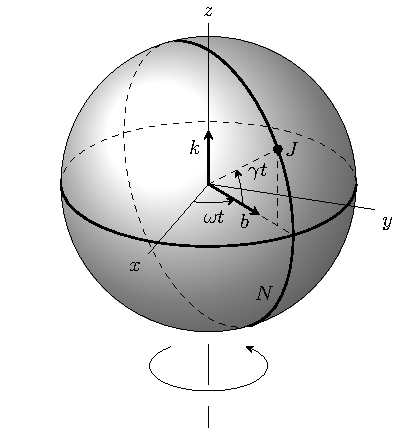
\includegraphics{sphereWithLines}
\caption{دو گھومتے حرکت کا خطی میل (مثال \حوالہ{مثال_الاحصاء_دو_گردش_کی_میل})}
\label{شکل_مثال_الاحصاء_دو_گردش_کی_میل}
\end{figure}
\انتہا{مثال}
%=================================

\حصہء{سوالات}
سوال \حوالہ{سوال_الاحصاء_تعین_گر_الف} تا سوال \حوالہ{سوال_الاحصاء_تعین_گر_ب} میں حرکت کرتی جسم کا تعین گر سمتیہ \عددی{\bM{r}(t)} ہے جہاں \عددی{t(>0)} وقت کو ظاہر کرتی ہے۔اس راہ کی شکل بیان کریں۔سمتیہ رفتار، رفتار اور اسراع دریافت کریں۔

%===================
\ابتدا{سوال}\شناخت{سوال_الاحصاء_تعین_گر_الف}\quad
$\bM{r}=t\bM{j}$\\
جوابات:
$\bM{v}=\bM{j},\quad \abs{\bM{v}}=1,\quad \bM{a}=0$
\انتہا{سوال}
%====================== 
\ابتدا{سوال}\quad
$\bM{r}=t^3\bM{j}$\\
جوابات:
$\bM{v}=3t^2\bM{j},\quad \abs{\bM{v}}=3t^2,\quad \bM{a}=6t\bM{j}$
\انتہا{سوال}
%====================== 
\ابتدا{سوال}\quad
$\bM{r}=(t^2-3t)\bM{j}$\\
جوابات:
$\bM{v}=(2t-3)\bM{j},\quad \abs{\bM{v}}=\abs{2t-3},\quad \bM{a}=2\bM{j}$
\انتہا{سوال}
%====================== 
\ابتدا{سوال}\quad
$\bM{r}=t^2\bM{i}-t\bM{j}$\\
جوابات:
$\bM{v}=2t\bM{i}-\bM{j},\quad \abs{\bM{v}}=\abs{\sqrt{4t^2+1}},\quad \bM{a}=2\bM{i}$
\انتہا{سوال}
%====================== 
\ابتدا{سوال}\quad
$\bM{r}=\cos t \,\bM{i}$\\
جوابات:
$\bM{v}=-\sin t\, \bM{j},\quad \abs{\bM{v}}=\abs{\sin t},\quad \bM{a}=-\cos t\,\bM{j}$
\انتہا{سوال}
%====================== 
\ابتدا{سوال}\quad
$\bM{r}=2\cos 5t \,\bM{i}-4\sin 3t \,\bM{j}$\\
جوابات:
$\bM{v}=-10\sin 5t\, \bM{i}-12\cos 3t\,\bM{j},\,\,\abs{\bM{v}}=\abs{\sqrt{100\sin^2 5t+144\cos^2 3t}}\\ \bM{a}=-50\cos 5t\,\bM{i}+36\sin 3t \,\bM{j}$
\انتہا{سوال}
%====================== 
\ابتدا{سوال}\quad
$\bM{r}=3\cos t^2 \,\bM{i}+2\sin t^2 \,\bM{j}$\\
جوابات:
$\bM{v}=-6t\sin t^2\, \bM{i}+4t\cos t^2\,\bM{j},\,\,\abs{\bM{v}}=\abs{\sqrt{36t^2\sin^2 t^2+16t^2\cos^2 t^2}}\\ 
\bM{a}=(-6\sin t^2-12t^2\cos t^2)\,\bM{i}+(4\cos t^2-8t^2\sin t^2) \,\bM{j}$
\انتہا{سوال}
%====================== 
\ابتدا{سوال}\شناخت{سوال_الاحصاء_تعین_گر_ب}\quad
$\bM{r}=5t^2 \,\bM{i}+3t \,\bM{j}+t^3\,\bM{k}$\\
جوابات:
$\bM{v}=10t\, \bM{i}+3\,\bM{j}+3t^2\,\bM{k},\,\,\abs{\bM{v}}=\abs{\sqrt{9t^4+100t^2+9}}\\ 
\bM{a}=10\,\bM{i}+6t \,\bM{k}$
\انتہا{سوال}
%====================== 
\ابتدا{سوال}زمین سے چاند تک کا فاصلہ \عددی{\SI{3.85e8}{\meter}} ہے اور زمین کے گرد چاند \عددی{27.322} دن یعنی \عددی{\SI{2.36e6}{\second}} میں ایک چکر پورا کرتا ہے۔زمین کے رخ چاند کی مرکز مائل اسراع دریافت کریں۔

جواب:\عددی{\abs{\bM{a}}=\SI{0.0027}{\meter\per\second\squared}} جو سطح زمین پر اسراع \عددی{g=\SI{9.8}{\meter\per\second\squared}} سے \عددی{3593} گنا کم ہے۔ 
\انتہا{سوال}
%=======================
\ابتدا{سوال}
وہ حرکت دریافت کریں جس کی اسراع مستقل قیمت ہو۔

جواب:
$\bM{r}(t)=\bM{a}_0\tfrac{t^2}{2}+\bM{v}_0t+\bM{x}_0$
جہاں \عددی{\bM{a}_0}، \عددی{\bM{v}_0} اور \عددی{\bM{x}_0} مستقل قیمتیں ہیں۔
\انتہا{سوال}
%=========================
\ابتدا{سوال}
\عددی{\bM{\omega}=\omega \bM{k}} اور \عددی{\bM{r}=R\cos \omega t\bM{i}+R\sin \omega t\bM{j}} لیتے ہوئے مساوات \حوالہ{مساوات_سمتیات_سمتی_رفتار_رداس_زاویائی_رفتار} کے تفرق  سے مساوات \حوالہ{مساوات_الاحصاء_اسراع_رفتار_حرکت} حاصل کریں۔
\انتہا{سوال}
%=======================
\ابتدا{سوال}
اگر ایک جسم کی حرکت \عددی{\bM{r}(t)} سے ظاہر کی جائے جہاں \عددی{t} وقت ہے تب \عددی{t=\phi{\tilde{t}}} تبادلے سے کیا مراد ہو گا؟

جواب:راہ تبدیل نہیں ہو گی البتہ راہ پر حرکت کی نوعیت تبدیل ہو گی۔
\انتہا{سوال}
%==========================

\حصہ{زنجیری ترکیب اور متعدد متغیرات کے تفاعل کا اوسط قیمت مسئلہ}\شناخت{حصہ_الاحصاء_زنجیری_ترکیب}
ہم متعدد متغیرات پر مبنی تفاعل کی خصوصیات پر غور کرتے ہیں۔ہم دو متغیرات کے تفاعل کو استعمال کرتے ہوئے  نتائج حاصل کریں گے جو زیادہ متغیرات کے تفاعل کے لئے بھی درست ہوں گے۔

نقطہ \عددی{(x_0,y_0)} پر تفاعل \عددی{f(x,y)}  اس صورت \اصطلاح{استمراری}\فرہنگ{استمراری}\حاشیہب{continuous}\فرہنگ{continuous} ہو گا جب اس نقطے کی \اصطلاح{پڑوس}\حاشیہد{پڑوس سے مراد \عددی{xy} سطح میں قرص \عددی{(x-x_0)^2+(y-y_0)^2<r^2} ہے جہاں \عددی{r>0} ہے۔} میں \عددی{f} معین ہو اور کسی بھی مثبت عدد \عددی{\epsilon} (جو غیر صفر اور کتنا ہی چھوٹا کیوں نا ہو) کے لئے ہم ایسا مثبت عدد \عددی{\sigma} تلاش کر سکتے ہیں کہ اس کے نقطے کی پڑوس  قرص 
\begin{align}
(x-x_0)^2+(y-y_0)^2<\sigma^2
\end{align}
میں تمام \عددی{(x,y)} پر درج ذیل ہو۔
\begin{align}
\abs{f(x,y)-f(x_0,y_0)}<\epsilon
\end{align}

جیومیٹریائی طور پر \عددی{(x_0,y_0)} پر \عددی{f(x,y)} کے استمراری ہونے سے مراد یہ ہے کہ \عددی{f(x_0,y_0)} کو قطع \عددی{2\epsilon} کا وسط لیتے ہوئے  ہم غیر صفر رداس \عددی{\sigma} کا ایسا قرص تلاش کر سکتے ہیں جس کا مرکز \عددی{(x_0,y_0)} ہو اور اس قرص  پر تمام \عددی{(x,y)} کا مطابقتی \عددی{f(x,y)} اس قطع پر پایا جاتا ہو (شکل \حوالہ{شکل_الاحصاء_استمرار_تعریف})۔
\begin{figure}
\centering
\begin{subfigure}{0.5\textwidth}
\centering
\begin{tikzpicture}
\draw(0,0)--++(2.5,0)node[below]{$x$};
\draw(0,0)--++(0,2.5)node[left]{$y$};
\draw(1.25,1.25)circle (1);
\draw[-stealth] (1.25,1.25)node[ocirc]{}node[below]{$(x_0,y_0)$} --++(30:1)node[pos=0.5,above]{$\sigma$};
\end{tikzpicture}
\end{subfigure}%
\begin{subfigure}{0.5\textwidth}
\centering
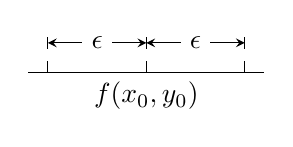
\begin{tikzpicture}
\draw(-1.5,0)--(1.5,0);
\draw(0,0)node[below]{$f(x_0,y_0)$}--++(0,0.15)++(0,0.15)--++(0,0.15);
\draw(-1.25,0)--++(0,0.15)++(0,0.15)--++(0,0.15);
\draw(1.25,0)--++(0,0.15)++(0,0.15)--++(0,0.15);
\draw[stealth-stealth](-1.25,0.15+0.15+0.15/2)--++(1.25,0)node[pos=0.5,fill=white]{$\epsilon$};
\draw[stealth-stealth](0,0.15+0.15+0.15/2)--++(1.25,0)node[pos=0.5,fill=white]{$\epsilon$};
\end{tikzpicture}
\end{subfigure}%
\caption{دو متغیرات کے تفاعل کی استمرار}
\label{شکل_الاحصاء_استمرار_تعریف}
\end{figure}

ہم ابتدائی علم الاحصاء سے جانتے ہیں کہ اگر \عددی{w} متغیر \عددی{x} کا قابل تفرق تفاعل ہو اور \عددی{x} از خود \عددی{t} کا قابل تفرق تفاعل ہو تب درج ذیل لکھا جا سکتا ہے جس کو تفرق کا زنجیری قاعدہ کہتے ہیں۔
\begin{align}
\frac{\dif w}{\dif t}=\frac{\dif w}{\dif x}\frac{\dif x}{\dif t}
\end{align} 
درج ذیل مسئلہ  تفرق کی زنجیری قاعدے کو عمومی بناتا ہے۔

%================
\ابتدا{مسئلہ}\شناخت{مسئلہ_الاحصاء_زنجیری_قاعدہ}\quad (زنجیری قاعدہ)\\
فرض کریں کہ \عددی{xy} سطح میں \اصطلاح{دائرہ کار}\فرہنگ{دائرہ کار}\حاشیہب{domain}\فرہنگ{domain}\فرہنگ{کھلا} \عددی{D}\حاشیہد{دائرہ کار \عددی{D} \ترچھا{جڑے ہوئے}  نقطوں کا \ترچھا{کھلا} سلسلہ ہے، جہاں \ترچھا{جڑا ہونے} \تحریر{(connected)} سے مراد یہ ہے کہ \عددی{D} کے کسی بھی دو نقطوں کو متناہی تعداد کے ایسے سیدھے قطعات سے ملایا جا سکتا ہے جن کے تمام نقطے \عددی{D} کا حصہ ہوں، اور \ترچھا{کھلا} \تحریر{(open)} سے مراد یہ ہے کہ \عددی{D} میں ہر نقطے کی پڑوس  کے تمام نقطے بھی \عددی{D} کا حصہ ہیں۔مثلاً کسی مستطیل یا دائرے کا اندرونی حصہ دائرہ کار ہو گا۔}\فرہنگ{جڑا ہوا}\فرہنگ{open}\فرہنگ{connected} میں تفاعل \عددی{w=f(x,y)} استمراری ہے  اور  اس تفاعل کے درجہ ایک جزوی تفرقات بھی \عددی{D} میں استمراری ہیں۔مزید فرض کریں کہ کسی وقفہ \عددی{T} میں \عددی{x=x(t)} اور \عددی{y=y(t)} قابل تفرق تفاعل ہیں جہاں \عددی{T} میں ہر \عددی{t} کا مطابقتی  نقطہ \عددی{[x(t),y(t)]}، دائرہ کار \عددی{D} میں پایا جاتا ہے۔ایسی صورت میں \عددی{T} میں تمام \عددی{t} کے لئے  \عددی{w=f[x(t),y(t)]} قابل تفرق ہو گا یعنی:
\begin{align}\label{مساوات_الاحصاء_زنجیری_تفرق_قاعدہ_الف}
\frac{\dif w}{\dif t}=\frac{\partial w}{\partial x}\frac{\dif x}{\dif t}+\frac{\partial w}{\partial y}\frac{\dif y}{\dif t}
\end{align}   
\انتہا{مسئلہ}
%======================
\ابتدا{ثبوت}
ہم \عددی{T} میں \عددی{t}  پر \عددی{\Delta t} اتنا چھوٹا چنتے ہیں کہ \عددی{t+\Delta t} بھی \عددی{T} کا حصہ ہو۔مزید ہم 
\begin{align}\label{مساوات_الاحصاء_زنجیری_الف}
\Delta x=x(t+\Delta t)-x(t),\quad \Delta y=y(t+\Delta t)-y(t)
\end{align} 
اور
\begin{align}\label{مساوات_الاحصاء_زنجیری_ب}
\Delta w=f(x+\Delta x,y+\Delta y)-f(x,y)
\end{align}
لیتے ہیں۔مساوات \حوالہ{مساوات_الاحصاء_زنجیری_ب} میں \عددی{f(x,y+\Delta y)} جمع اور منفی کرتے ہوئے درج ذیل لکھا جا سکتا ہے۔
\begin{align*}
\Delta w=[f(x+\Delta x,y+\Delta y)-f(x,y+\Delta y)]+[f(x,y+\Delta y)-f(x,y)]
\end{align*}
درج بالا مساوات کے قوسین پر باری باری ایک متغیر کے تفاعل کا اوسط قیمت مسئلہ لاگو کرتے ہوئے
\begin{align}\label{مساوات_الاحصاء_زنجیری_پ}
\Delta w=\Delta x \left.\frac{\partial f}{\partial x} \right|_{x_1,y+\Delta y}+\Delta y \left.\frac{\partial f}{\partial y} \right|_{x,y_1}
\end{align}  
حاصل ہوتا ہے جہاں \عددی{x} اور \عددی{x+\Delta x} کے درمیان کہیں \عددی{x_1} پایا جاتا ہے، \عددی{y} اور \عددی{y+\Delta y} کے درمیان کہیں \عددی{y_1} پایا جاتا ہے۔مساوات \حوالہ{مساوات_الاحصاء_زنجیری_پ} کے دونوں اطراف کو \عددی{\Delta t} سے تقسیم کرتے اور \عددی{\Delta t \to 0} لیتے ہوئے، اور چونکہ
 \عددی{\tfrac{\partial f}{\partial x}} اور \عددی{\tfrac{\partial f}{\partial y}} کو استمراری تصور کیا گیا ہے، مساوات  \حوالہ{مساوات_الاحصاء_زنجیری_الف} حاصل ہوتا ہے۔
\انتہا{ثبوت}
%========================

درج بالا مسئلے کو وسعت دیتے ہوئے درج ذیل مسئلہ اخذ کیا جا سکتا ہے۔

%==========
\ابتدا{مسئلہ}\شناخت{مسئلہ_الاحصاء_جزوی_تفرقات}
فرض کریں کہ \عددی{xy} سطح میں \اصطلاح{دائرہ کار} \عددی{D} پر تفاعل \عددی{w=f(x,y)} استمراری ہے  اور  اس تفاعل کے درجہ ایک جزوی تفرقات بھی \عددی{D} میں استمراری ہیں۔مزید فرض کریں کہ \عددی{uv} سطح میں کسی وقفہ \عددی{B} میں \عددی{x=x(u,v)} اور \عددی{y=y(u,v)} قابل جزوی تفرق تفاعل ہیں جہاں \عددی{B} میں ہر \عددی{(u,v)} کا مطابقتی نقطہ \عددی{[x(u,v),y(u,v)]}، دائرہ کار \عددی{D} میں پایا جاتا ہے۔ایسی صورت میں \عددی{B} میں تفاعل  \عددی{w=f[x(u,v),y(u,v)]} معین ہو گا اور \عددی{B} میں تمام \عددی{u} اور \عددی{v} کے لئے اس تفاعل کے جزوی تفرقات  درج ذیل ہوں گے۔
\begin{gather}
\begin{aligned}\label{مساوات_الاحصاء_زنجیری_ترکیب_کلیات}
\frac{\partial w}{\partial u}&=\frac{\partial w}{\partial x}\frac{\partial x}{\partial u}+\frac{\partial w}{\partial y}\frac{\partial y}{\partial u}\\
\frac{\partial w}{\partial v}&=\frac{\partial w}{\partial x}\frac{\partial x}{\partial v}+\frac{\partial w}{\partial y}\frac{\partial y}{\partial v}
\end{aligned}
\end{gather}
\انتہا{مسئلہ}
%====================

\عددی{u} یا \عددی{v} کو غیر متغیر رکھتے ہوئے مسئلہ \حوالہ{مسئلہ_الاحصاء_زنجیری_قاعدہ} کے اطلاق سے  درج بالا مسئلہ ثابت ہوتا ہے۔

ابتدائی علم الاحصاء  سے ہم جانتے ہیں کہ قابل تفرق تفاعل \عددی{f(x)} کے لئے درج ذیل لکھا جا سکتا ہے جہاں \عددی{x_0} اور \عددی{x_0+h} کے درمیان موزوں نقطے پر تفرق لیا جاتا ہے۔
\begin{align*}
f(x_0+h)-f(x_0)=h\frac{\dif f}{\dif x}
\end{align*}
اس کو احصاء تفرقیات کا مسئلہ اوسط قیمت کہتے ہیں جس کو  وسعت دے کر  دو متغیرات کے تفاعل پر لاگو  کیا جا سکتا ہے۔

%==================
\ابتدا{مسئلہ}\شناخت{مسئلہ_الاحصاء_اوسط_قیمت}\quad (مسئلہ اوسط قیمت)\\
فرض کریں کہ دائرہ کار \عددی{D} میں تفاعل \عددی{f(x,y)} استمراری ہے اور اس تفاعل کے درجہ ایک جزوی تفرقات بھی \عددی{D} میں استمراری ہیں۔ مزید فرض کریں کہ \عددی{(x_0,y_0)} اور  \عددی{(x_0+h,y_0+k)} دائرہ کار \عددی{D} میں پائے جانے والے ایسے نقطے ہیں کہ انہیں جوڑنے والا سیدھا قطع  بھی \عددی{D} میں پائی جاتی ہو (شکل \حوالہ{شکل_مسئلہ_الاحصاء_اوسط_قیمت})۔ایسی صورت میں 
\begin{align}\label{مساوات_الاحصاء_مسئلہ_زنجیری_الف}
f(x_0+h,y_0+k)-f(x_0,y_0)=h\frac{\partial f}{\partial x}+k\frac{\partial f}{\partial y}
\end{align}
لکھا جا سکتا ہے جہاں جزوی تفرقات کو  اس قطع پر موزوں نقطے پر حاصل کیا جاتا ہے۔
\begin{figure}
\centering
\begin{tikzpicture}
\draw[smooth cycle] plot coordinates {(0,0)(-2,0.75)(-1,1.75)(0,2)(1.5,2)(3.2,1.75)(2,0.25)};
\draw(0,0.7)node[ocirc]{}node[below]{$(x_0,y_0)$}--(1.5,1)node[ocirc]{}node[above]{$(x_0+h,y_0+k)$};
\draw(0,1.75)node{$D$};
\end{tikzpicture}
\caption{مسئلہ اوسط قیمت}
\label{شکل_مسئلہ_الاحصاء_اوسط_قیمت}
\end{figure}
\انتہا{مسئلہ}
%======================
\ابتدا{ثبوت}
درج ذیل
\begin{align*}
x&=x_0+th,\quad y=y_0+tk\quad (0\le t \le 1)\\
F(t)&=f(x_0+th,y_0+tk)
\end{align*}
سے
\begin{align*}
f(x_0+h,y_0+k)=F(1),\quad f(x_0,y_0)=F(0)
\end{align*}
لکھا جا سکتا ہے۔ایک متغیر تفاعل کے  مسئلہ اوسط قیمت کے تحت \عددی{0} اور \عددی{1} کے درمیان  ایسی قیمت \عددی{t_1}  پائی جاتی ہے جس کے لئے  درج ذیل لکھا جا سکتا ہے۔ 
\begin{align}\label{مساوات_الاحصاء_مسئلہ_زنجیری_ب}
f(x_0+h,y_0+k)-f(x_0,y_0)=F(1)-F(0)=F'(t_1)
\end{align}
اب چونکہ \عددی{\tfrac{\dif x}{\dif t}=h} اور \عددی{\tfrac{\dif y}{\dif t}=k} ہیں لہٰذا مسئلہ \حوالہ{مسئلہ_الاحصاء_زنجیری_قاعدہ} کے تحت
\begin{align}\label{مساوات_الاحصاء_مسئلہ_زنجیری_پ}
F'=\frac{\partial f}{\partial x}h+\frac{\partial f}{\partial y}k
\end{align}
ہو گا جہاں دائیں ہاتھ تفرقات کو نقطہ \عددی{(x_0+t_1h,y_0+t_1k)} پر حاصل کیا جائے گا جو اس قطع پر واقع ہے جس کے سر \عددی{(x_0,y_0)} اور \عددی{(x_0+h,y_0+k)} ہیں۔مساوات \حوالہ{مساوات_الاحصاء_مسئلہ_زنجیری_پ} کو مساوات \حوالہ{مساوات_الاحصاء_مسئلہ_زنجیری_ب} میں پر کرنے سے  مساوات \حوالہ{مساوات_الاحصاء_مسئلہ_زنجیری_الف} حاصل ہوتا ہے۔
\انتہا{ثبوت}
%========================

تین متغیرات کے تفاعل \عددی{f(x,y,z)} جو مسئلہ \حوالہ{مسئلہ_الاحصاء_اوسط_قیمت} میں دیے گئے شرائط کے مماثل شرائط پر پورا اترتا ہو کے لئے بالکل اسی مسئلے کی طرح درج ذیل لکھا جا سکتا ہے
\begin{align}\label{مساوات_الاحصاء_مسئلہ_زنجیری_ت}
f(x_0+h,y_0+k,z_0+l)-f(x_0,y_0,z_0)=h\frac{\partial f}{\partial x}+k\frac{\partial f}{\partial y}+l\frac{\partial f}{\partial z}
\end{align}
جہاں جزوی تفرقات کو \عددی{(x_0,y_0,z_0)} تا \عددی{(x_0+h,y_0+k,z_0+l)} قطع پر موزوں نقطے پر حاصل کیا جائے گا۔

%===================
\حصہء{سوالات}
سوال \حوالہ{سوال_الاحصاء_زنجیری_قاعدہ_الف} تا سوال \حوالہ{سوال_الاحصاء_زنجیری_قاعدہ_ب} میں مساوات \حوالہ{مساوات_الاحصاء_زنجیری_تفرق_قاعدہ_الف} کی مدد سے \عددی{\tfrac{\dif w}{\dif t}} دریافت کریں۔

%===============
\ابتدا{سوال}\شناخت{سوال_الاحصاء_زنجیری_قاعدہ_الف}\quad
$w=x-y,\quad x=t,\quad y=\ln t$\\
جواب:
$1-\tfrac{1}{t}$
\انتہا{سوال}
%========================
\ابتدا{سوال}\quad
$w=\sqrt{x^2+y^2},\quad x=e^{-t},\quad y=e^{t}$\\
جواب:
$\tfrac{e^{2t}-e^{-2t}}{\sqrt{e^{2t}+e^{-2t}}}$
\انتہا{سوال}
%========================
\ابتدا{سوال}\quad
$w=\tfrac{x}{y},\quad x=g(t),\quad y=h{t}$\\
جواب:
$\tfrac{g'h-gh'}{h^2}$
\انتہا{سوال}
%========================
\ابتدا{سوال}\شناخت{سوال_الاحصاء_زنجیری_قاعدہ_ب}\quad
$w=\tfrac{x}{y},\quad x=\cos t,\quad y=\sin t$\\
جواب:
$-\cosec^{\,2} t$
\انتہا{سوال}
%========================
\ابتدا{سوال}
فرض کریں کہ \عددی{w=f(x,y,z)} ہے جہاں \عددی{x}، \عددی{y} اور \عددی{z} از خود \عددی{t} کے تفاعل ہیں۔ثابت کریں کہ مسئلہ \حوالہ{مسئلہ_الاحصاء_زنجیری_قاعدہ} کی طرز کے شرائط کی صورت میں درج ذیل ہو گا۔
\begin{align}\label{مساوات_الاحصاء_زنجیری_تین_متغیرات}
\frac{\dif w}{\dif t}=\frac{\partial w}{\partial x}\frac{\dif x}{\dif t}+\frac{\partial w}{\partial y}\frac{\dif y}{\dif t}+\frac{\partial w}{\partial z}\frac{\dif z}{\dif t}
\end{align}
\انتہا{سوال}
%===================
سوال \حوالہ{سوال_الاحصاء_زنجیری_تین_متغیرات_الف} اور سوال \حوالہ{سوال_الاحصاء_زنجیری_تین_متغیرات_ب} میں مساوات \حوالہ{مساوات_الاحصاء_زنجیری_تین_متغیرات} کی مدد سے \عددی{\tfrac{\dif w}{\dif t}} دریافت کریں۔

%==========================
\ابتدا{سوال}\شناخت{سوال_الاحصاء_زنجیری_تین_متغیرات_الف}\quad
$w=x^2+y^2+z^2,\quad x=t^2,\quad y=\ln t,\quad z=e^t$\\
جواب:
$\tfrac{2}{t}\ln t+2e^{2t}+4t^3$
\انتہا{سوال}
%=========================
\ابتدا{سوال}\شناخت{سوال_الاحصاء_زنجیری_تین_متغیرات_ب}\quad
$w=\sqrt{x^2+y^2+z^2},\quad x=\cos t,\quad y=\sin t,\quad z=t$\\
جواب:
$\tfrac{t}{\sqrt{1+t^2}}$
\انتہا{سوال}
%=========================
\ابتدا{سوال}
مسئلہ \حوالہ{مسئلہ_الاحصاء_جزوی_تفرقات} کو ثابت کریں۔
\انتہا{سوال}
%=======================
سوال \حوالہ{سوال_الاحصاء_جزوی_تفرقات_الف} تا سوال \حوالہ{سوال_الاحصاء_جزوی_تفرقات_ب} میں \عددی{\tfrac{\partial w}{\partial u}} اور \عددی{\tfrac{\partial w}{\partial v}} دریافت کریں۔

%===================
\ابتدا{سوال}\شناخت{سوال_الاحصاء_جزوی_تفرقات_الف}\quad
$w=\ln(x^2+y^2),\quad x=e^u\cos v,\quad y=e^u\sin v$\\
جواب:
$2,\,\, 0$
\انتہا{سوال}
%======================
\ابتدا{سوال}\quad
$w=xy,\quad x=e^u\cos v,\quad y=e^u\sin v$\\
جواب:
$e^{2u}\sin 2v,\,\,e^{2u}\cos 2v$
\انتہا{سوال}
%======================
\ابتدا{سوال}\شناخت{سوال_الاحصاء_جزوی_تفرقات_ب}\quad
$w=x^2-y^2,\quad x=u^2-v^2,\quad y=2uv$\\
جواب:
$4u(u^2-3v^2),\,\,4v(v^2-3u^2)$
\انتہا{سوال}
%======================
\ابتدا{سوال}
مساوات \حوالہ{مساوات_الاحصاء_مسئلہ_زنجیری_ت} حاصل کریں۔
\انتہا{سوال}
%======================
\ابتدا{سوال}
فرض کریں کہ \عددی{w=f(x,y)} ہے جہاں \عددی{x=r\cos \theta} اور \عددی{y=r\sin \theta} ہیں۔درج ذیل ثابت کریں۔
\begin{align*}
\left(\frac{\partial w}{\partial r}\right)^2+\frac{1}{r^2}\left(\frac{\partial w}{\partial \theta}\right)^2=\left(\frac{\partial w}{\partial x}\right)^2+\left(\frac{\partial w}{\partial y}\right)^2
\end{align*}
جواب:درج ذیل استعمال کرتے ہوئے با آسانی ثابت ہو گا۔
\begin{align*}
\frac{\partial w}{\partial r}&=\frac{\partial w}{\partial x}\frac{\partial x}{\partial r}+\frac{\partial w}{\partial y}\frac{\partial y}{\partial r}=
\frac{\partial w}{\partial x}\cos \theta +\frac{\partial w}{\partial y}\sin \theta \\
\frac{\partial w}{\partial \theta}&=\frac{\partial w}{\partial x}\frac{\partial x}{\partial \theta}+\frac{\partial w}{\partial y}\frac{\partial y}{\partial \theta}=
-\frac{\partial w}{\partial x}r\sin \theta +\frac{\partial w}{\partial y}r\cos\theta 
\end{align*}
\انتہا{سوال}
%======================
\ابتدا{سوال}
فرض کریں کہ \عددی{w=f(v,z)}ہے جہاں  \عددی{v=x+ct} اور  \عددی{z=x-ct} ہیں جبکہ  \عددی{c} مستقل قیمت  ہے۔درج ذیل ثابت کریں جہاں تمام تفرقات کو ممکن تصور کریں۔ \عددی{w_{xx}} سے مراد \عددی{\tfrac{\partial ^2 w}{\partial x^2}} ہے۔
\begin{align*}
c^2w_{xx}-w_{tt}=4c^2w_{vz}
\end{align*} 
\انتہا{سوال}
%=========================
\ابتدا{سوال}
فرض کریں کہ \عددی{w=f(x,y)} ہے جہاں \عددی{x=r\cos \theta} اور \عددی{y=r\sin \theta} ہیں۔درج ذیل ثابت کریں۔
\begin{align*}
w_{xx}+w_{yy}=w_{rr}+\frac{1}{r}w_r+\frac{1}{r^2}w_{\theta \theta}
\end{align*}
جواب:
$r=\sqrt{x^2+y^2}$
اور
$\theta=\tan^{-1}\frac{y}{x}$
سے درج ذیل حاصل کرتے ہوئے ثابت ہو گا۔
\begin{align*}
r_x&=\frac{x}{r},\,\, \theta_x=-\frac{y}{r^2},\,\, r_{xx}=\frac{y^2}{r^3},\quad \text{وغیرہ}\\
 w_{xx}&=x^2r^{-2}w_{rr}-2xyr^{-3}w_{r\theta}+y^2r^{-4}w_{\theta\theta}+y^2r^{-3}w_r+2xyr^{-4}w_{\theta},\quad \text{وغیرہ}
\end{align*}
\انتہا{سوال}
%=======================

\حصہ{سمتی تفرق، غیر سمتی میدان کی ڈھلوان}\شناخت{حصہ_الاحصاء_ڈھلوان}
ہم فضا میں غیر سمتی میدان \عددی{f(P)=f(x,y,z)}  پر غور کرتے ہیں (حصہ \حوالہ{حصہ_الاحصاء_غیر_سمتی-_اور_سمتی_میدان})۔ہم جانتے ہیں کہ  \عددی{x}، \عددی{y} اور \عددی{z}  رخ  میں تفاعل کی تبدیلی کی شرح بالترتیب \عددی{\tfrac{\partial f}{\partial x}}، \عددی{\tfrac{\partial f}{\partial y}} اور \عددی{\tfrac{\partial f}{\partial z}} ہے۔ آئیں کسی بھی رخ اس تفاعل کی تبدیلی کی شرح یعنی \اصطلاح{سمتی تفرق} حاصل کریں۔

ہم فضا میں کوئی نقطہ \عددی{P} اور اس نقطے پر کوئی رخ چنتے ہیں۔اس رخ  کو اکائی سمتیہ \عددی{\bM{b}} سے ظاہر کرتے ہیں۔نقطہ \عددی{P} سے \عددی{s} فاصلے پر  \عددی{\bM{b}} کی رخ سیدھے خط \عددی{C} پر نقطہ \عددی{Q} پایا جاتا ہے (شکل \حوالہ{شکل_الاحصاء_سمتی_تفرق})۔اگر درج ذیل حد
\begin{align}\label{مساوات_الاحصاء_سمتی_تفرق_الف}
\frac{\partial f}{\partial s}=\lim_{s\to 0}\frac{f(Q)-f(P)}{s}
\end{align}
موجود ہو تب اس کو \عددی{P} پر \عددی{\bM{b}} کی رخ \عددی{f} کی \اصطلاح{سمتی تفرق}\فرہنگ{سمتی!تفرق}\فرہنگ{تفرق!سمتی}\حاشیہب{directional derivative}\فرہنگ{directional derivative}\فرہنگ{derivative!directional} کہتے ہیں۔ظاہر ہے کہ \عددی{\tfrac{\partial f}{\partial s}} در حقیقت \عددی{P} پر \عددی{\bM{b}} کی رخ  \عددی{f} کی شرح تبدیلی ہے۔ 
\begin{figure}
\centering
\begin{tikzpicture}
\pgfmathsetmacro{\ang}{20}
\draw(0,0)--++(\ang:3.5)node[below]{$C$};
\draw(0,0)node[below]{$P$}--++(\ang:2)node[ocirc]{}node[below]{$Q$};
\draw[-latex](0,0)node[ocirc]{}--++(\ang:1)node[below]{$\bM{b}$};
\draw [decorate,decoration={brace,amplitude=5pt},shift={(\ang+90:5pt)}](0,0) --++(\ang:1)node [black,midway,shift={(\ang+90:9pt)}] {\footnotesize$s$};
\end{tikzpicture}
\caption{سمتی تفرق}
\label{شکل_الاحصاء_سمتی_تفرق}
\end{figure}

یوں \عددی{P} پر \عددی{f} کے لامتناہی تعداد میں سمتی تفرقات پائے جاتے ہیں۔اگر \عددی{P} کا تعین گر سمتیہ \عددی{\bM{a}} ہو تب \عددی{C}  کو درج ذیل لکھا جا سکتا ہے 
\begin{align}\label{مساوات_الاحصاء_سمتی_تفرق_ب}
\bM{r}(s)=x(x)\bM{i}+y(s)\bM{j}+z(s)\bM{k}=\bM{a}+s\bM{b}\quad \quad (s\ge 0)
\end{align}
اور \عددی{\tfrac{\partial f}{\partial s}} سے مراد \عددی{C} پر \عددی{f[x(s),y(s),z(s)]} کا لمبائی \عددی{s} کے ساتھ تفرق ہے۔اب اگر \عددی{f} کے استمراری جزوی تفرقات پائے جاتے ہوں تب زنجیری قاعدے (مسئلہ \حوالہ{مسئلہ_الاحصاء_زنجیری_قاعدہ}) کے تحت درج ذیل لکھا جا سکتا ہے
\begin{align}\label{مساوات_الاحصاء_سمتی_تفرق_پ}
\frac{\partial f}{\partial s}=\frac{\partial f}{\partial x}x'+\frac{\partial f}{\partial y}y'+\frac{\partial f}{\partial z}z'
\end{align}
جہاں \عددی{x'=\tfrac{\dif x}{\dif s}}  کو \عددی{s=0} پر حاصل کیا جاتا ہے۔اب مساوات \حوالہ{مساوات_الاحصاء_سمتی_تفرق_ب} سے
\begin{align*}
\bM{r}'=x'\bM{i}+y'\bM{j}+z'\bM{k}=\bM{b}
\end{align*}
لکھا جا سکتا ہے جس کو دیکھ کر  خیال آتا ہے کہ  سمتیہ
\begin{align}\label{مساوات_الاحصاء_سمتی_تفرق_ت}
f_{\text{ڈھلوان}}=\frac{\partial f}{\partial x}\bM{i}+\frac{\partial f}{\partial y}\bM{j}+\frac{\partial f}{\partial z}\bM{k}
\end{align}
متعارف کرنے سے مساوات \حوالہ{مساوات_الاحصاء_سمتی_تفرق_پ} کو اندرونی ضرب (ضرب نقطہ) کی صورت میں لکھا جا سکتا ہے۔
\begin{align}\label{مساوات_الاحصاء_سمتی_تفرق_ٹ}
\frac{\partial f}{\partial s}=\bM{b}\cdot f_{\text{ڈھلوان}} \quad \quad (\abs{\bM{b}}=1)
\end{align}
سمتیہ 
$f_{\text{ڈھلون}}$
کو غیر سمتی تفاعل \عددی{f} کی \اصطلاح{ڈھلوان}\فرہنگ{ڈھلوان}\حاشیہب{gradient}\فرہنگ{gradient} کہتے ہیں۔

تفرقی عامل \عددی{\nabla}\حاشیہد{\عددی{\nabla} یونانی حرف تہجی ہے جو نیبلا کہلاتا ہے۔}
\begin{align*}
\nabla =\frac{\partial}{\partial x}\bM{i}+\frac{\partial}{\partial y}\bM{j}+\frac{\partial}{\partial z}\bM{k}
\end{align*}
متعارف کرتے ہوئے  مساوات \حوالہ{مساوات_الاحصاء_سمتی_تفرق_ت} کو 
\begin{align}\label{مساوات_الاحصاء_سمتی_تفرق_ث}
f_{\text{ڈھلوان}}=\nabla f=\frac{\partial f}{\partial x}\bM{i}+\frac{\partial f}{\partial y}\bM{j}+\frac{\partial f}{\partial z}\bM{k}
\end{align}
اور مساوات \حوالہ{مساوات_الاحصاء_سمتی_تفرق_ٹ} کو 
\begin{align}\label{مساوات_الاحصاء_سمتی_تفرق_ج}
\frac{\partial f}{\partial s}=\bM{b}\cdot \nabla f\quad \quad (\abs{\bM{b}}=1)
\end{align}
لکھا جا سکتا ہے۔

اگر \عددی{\bM{b}} کارتیسی \عددی{x} محور کی رخ ہو تب \عددی{\bM{b}=\bM{i}} ہو گا اور \عددی{f} کا سمتی تفرق درج ذیل ہو گا۔
\begin{align*}
\frac{\partial f}{\partial s}=\bM{b}\cdot \nabla f=\frac{\partial f}{\partial x}\bM{i}\cdot \bM{i}=\frac{\partial f}{\partial x}
\end{align*}
اسی طرح مثبت \عددی{y} اور مثبت \عددی{z} محور کی رخ سمتی تفرق بالترتیب \عددی{\tfrac{\partial f}{\partial y}} اور \عددی{\tfrac{\partial f}{\partial z}} ہوں گے۔

%==================
\ابتدا{مثال}\quad سمتی تفرق\\
غیر سمتی تفاعل \عددی{f(x,y,z)=x^2+2y-z^3} کا نقطہ \عددی{P:(-2,1,3)} پر \عددی{\bM{a}=3\bM{i}-4\bM{j}} کی رخ سمتی تفرق دریافت کریں۔

حل:چونکہ \عددی{\abs{\bM{a}}=5} ہے لہٰذا \عددی{\bM{a}} کی رخ اکائی سمتیہ
 \عددی{\bM{b}=\tfrac{\bM{a}}{\abs{\bM{a}}}=\tfrac{3}{5}\bM{i}-\tfrac{4}{5}\bM{j}} ہو گا۔ \عددی{f} کی ڈھلوان درج ذیل ہے۔
\begin{align*}
\nabla f=2x\bM{i}+2\bM{j}-3z^2\bM{k}\implies  \nabla f(P)=-4\bM{i}+2\bM{j}-27\bM{k}
\end{align*}
یوں نقطہ \عددی{P} پر \عددی{\bM{a}} کی رخ سمتی تفرق درج ذیل ملتا ہے۔
\begin{align*}
\frac{\partial f}{\partial s}=\bM{b}\cdot \nabla f=\frac{1}{5}(3\bM{i}-4\bM{j})\cdot (-4\bM{i}+2\bM{j}-27\bM{k})=-4
\end{align*}
حاصل جواب منفی ہے جس کا مطلب ہے کہ \عددی{\bM{a}} کی رخ  \عددی{f} گھٹتا ہے۔
\انتہا{مثال}
%========================

ہم اب ثابت کرتے ہیں کہ \عددی{\nabla f} کی قیمت اور رخ پر چنے گئے کارتیسی نظام کا کوئی اثر نہیں پایا جاتا ہے۔ 

مساوات \حوالہ{مساوات_الاحصاء_سمتی_تفرق_ت} سمتی تفرق دیتا ہے جو کسی دوسرے کارتیسی نظام میں درج ذیل لکھا جائے گا
\begin{align*}
f_{\text{ڈھلوان}}=\frac{\partial f}{\partial x^*}\bM{i}^*+\frac{\partial f}{\partial y^*}\bM{j}^*+\frac{\partial f}{\partial z^*}\bM{k}^*
\end{align*}
 جہاں \عددی{x^*}، \عددی{y^*} اور \عددی{z^*} دوسرے نظام کے محور جبکہ \عددی{\bM{i}^*}، \عددی{\bM{j}^*} اور \عددی{\bM{k}^*} اس کے مطابقتی اکائی سمتیات ہیں۔ان مساوات میں جزوی تفرقات پائے جاتے ہیں اور یہ کہنا مشکل ہو گا کہ دونوں مساوات سے یکساں ڈھلوان حاصل ہو گا۔ 

اب غیر سمتی تفاعل کی تعریف کے تحت نقطہ \عددی{P} پر \عددی{f} کی قیمت کا دارومدار \عددی{P} پر ہے نا کہ چنے گئے کارتیسی نظام پر۔اسی طرح \عددی{C} پر لمبائی \عددی{s} پر بھی چنے گئے کارتیسی نظام کا کوئی اثر نہیں پایا جاتا ہے۔یوں \عددی{\tfrac{\partial f}{\partial s}} پر چنے گئے کارتیسی نظام کا کوئی اثر نہیں ہو گا۔ اب مساوات \حوالہ{مساوات_الاحصاء_سمتی_تفرق_ج} کو درج ذیل لکھا جا سکتا ہے
\begin{align*}
\frac{\partial f}{\partial s}=\abs{\bM{b}}\abs{\nabla f}\cos \gamma=\abs{\nabla f}\cos \gamma
\end{align*}
جہاں \عددی{\bM{b}} اور \عددی{\nabla f} کے مابین زاویہ \عددی{\gamma} ہے۔ہم دیکھتے ہیں کہ  \عددی{\cos \gamma=1} یعنی \عددی{\gamma=0} پر \عددی{\tfrac{\partial f}{\partial s}} کی زیادہ سے زیادہ قیمت \عددی{\tfrac{\partial f}{\partial s}=\abs{\nabla f}} پائی جاتی ہے۔اب چونکہ \عددی{\tfrac{\partial f}{\partial s}} غیر متغیر ہے لہٰذا \عددی{\nabla f}  کی قیمت اور سمت پر کارتیسی نظام کا کوئی اثر نہیں ہو گا۔اس سے درج ذیل نتیجہ ملتا ہے۔

%===============
\ابتدا{مسئلہ}\quad ڈھلوان\\
ایسا غیر سمتی تفاعل \عددی{f(P)=f(x,y,z)}  جس کے استمراری ایک درجی جزوی تفرقات پائے جاتے ہوں کی ڈھلوان موجود ہے جس کی لمبائی اور رخ پر چنے گئے کارتیسی نظام محدد کا کوئی اثر نہیں پایا جاتا ہے۔اگر نقطہ \عددی{P} پر \عددی{f} کی ڈھلوان غیر صفر سمتیہ ہو تب \عددی{P} پر \عددی{f} کی زیادہ سے زیادہ تبدیلی ڈھلوان کی رخ ہو گی۔ 
\انتہا{مسئلہ}
%========================

ڈھلوان کی دوسری جیومیٹریائی خصلت جانتے ہیں۔فضا میں قابل تفرق غیر سمتی تفاعل \عددی{f(x,y,z)} پر غور کرتے ہیں۔ہر مستقل \عددی{c} کے لئے مساوات
\begin{align}\label{مساوات_الاحصاء_سمتی_تفرق_چ}
f(x,y,z)=c=\text{مستقل}
\end{align}
 سطح \عددی{S} کو ظاہر کرتا ہے۔\عددی{c} کے تمام قیمتیں لیتے ہوئے ہمیں نسل سطح ملتا ہے جنہیں \عددی{f} کی \اصطلاح{ہموار سطحیں}\فرہنگ{ہموار سطحیں}\حاشیہب{level surfaces}\فرہنگ{level surfaces} کہتے ہیں۔ تفاعل کی تعریف کے تحت، فضا میں کسی بھی نقطے پر  \عددی{f} کی قیمت منفرد ہو گی لہٰذا فضا میں ہر نقطے سے \عددی{f} کی صرف اور صرف ایک ہموار سطح گزرے گی۔ہم جانتے ہیں کہ فضا میں کسی بھی منحنی \عددی{C} کو درج ذیل لکھا جا سکتا ہے (حصہ \حوالہ{حصہ_الاحصاء_لمبائی_قوس})۔
\begin{align}\label{مساوات_الاحصاء_سمتی_تفرق_ح}
\bM{r}(t)=x(t)\bM{i}+y(t)\bM{j}+z(t)\bM{k}
\end{align}
اب اگر \عددی{C} کو \عددی{S} پر رہنے کا پابند بنایا جائے تب مساوات \حوالہ{مساوات_الاحصاء_سمتی_تفرق_ح} میں تفاعل \عددی{x(t)}، \عددی{y(t)} اور \عددی{z(t)} کو مساوات \حوالہ{مساوات_الاحصاء_سمتی_تفرق_چ} پر پورا اترنا ہو گا یعنی:
\begin{align}\label{مساوات_الاحصاء_سمتی_تفرق_خ}
f[x(t),y(t),z(t)]=c
\end{align}
زنجیری تفرق  (مسئلہ \حوالہ{مسئلہ_الاحصاء_زنجیری_قاعدہ}) استعمال کرتے ہوئے مساوات \حوالہ{مساوات_الاحصاء_سمتی_تفرق_خ} کا \عددی{t} کے ساتھ تفرق لیتے ہیں
\begin{align}\label{مساوات_الاحصاء_سمتی_تفرق_د}
\frac{\partial f}{\partial x}\dot{x}+\frac{\partial f}{\partial y}\dot{y}+\frac{\partial f}{\partial z}\dot{z}=(\nabla f)\cdot \dot{\bM{r}}=0
\end{align}
جہاں سمتیہ
\begin{align*}
\dot{\bM{r}}=\dot{x}\bM{i}+\dot{y}\bM{j}+\dot{z}\bM{k}
\end{align*}
منحنی \عددی{C} کا مماس ہے (حصہ \حوالہ{حصہ_الاحصاء_مماس_انحنا_مروڑ})۔ \عددی{S} پر مختلف سمتوں میں نقطہ \عددی{P} سے  گزرتی منحنی کے مماس، \عددی{P} پر \عددی{S} کو چھوتی سطح مستوی سے گزریں گے۔اس سطح مستوی کو \عددی{P} پر \عددی{S} کی \اصطلاح{مماسی سطح}\فرہنگ{مماسی!سطح}\فرہنگ{سطح!مماس}\حاشیہب{tangent plane}\فرہنگ{tangent plane} کہتے ہیں۔ مماسی سطح کے عمودی، نقطہ \عددی{P} سے گزرتا خط، \عددی{P} پر \عددی{S} کا \اصطلاح{عمود}\فرہنگ{عمود}\حاشیہب{normal}\فرہنگ{normal} کہلاتا ہے (شکل \حوالہ{شکل_الاحصاء_ڈھلوان})۔ صفحہ \حوالہصفحہ{مسئلہ_الجبرا_قائمیت} پر مسئلہ \حوالہ{مسئلہ_الجبرا_قائمیت} کی مدد سے درج ذیل نتیجہ ملتا ہے۔
\begin{figure}
\centering
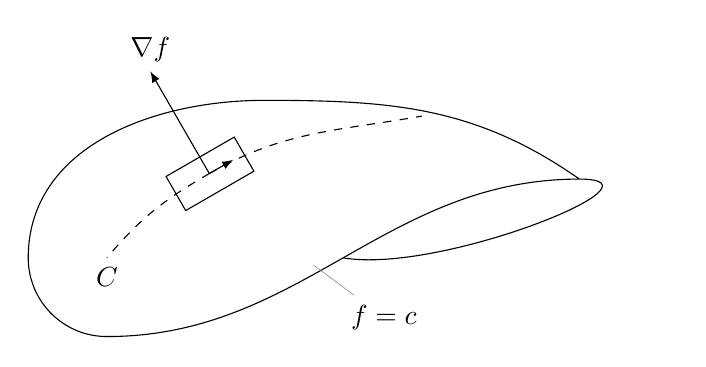
\begin{tikzpicture}
\pgfmathsetmacro{\ang}{30}
%\draw (0,-2) grid ++(7,3);
\draw(7,0) to [out=145,in=0] (3,1) to [out=180,in=90] (0,-1) to [out=-90,in=180] (1,-2) to [out=0,in=180] (7,0);
\draw(4,-1) to [out=-10,in=0] (7,0);
\draw[dashed] (2.3,0.07) to [out=\ang,in=-170] (5,0.8);
\draw[dashed] (2.3,0.07) to [out=\ang-180,in=50] (1,-1)node[below]{$C$};
\draw (3.5,-1)node[pin={[pin distance=0.5cm]-45:{$f=c$}}]{};
\draw(2,-0.4)--++(\ang:1)--++(\ang+90:0.5)--++(\ang:-1)--++(\ang-90:0.5);
\draw[-latex](2.3,0.07)--++(\ang:0.35);
\draw[-latex](2.3,0.07)--++(\ang+90:1.5)node[above]{$\nabla f$};
\end{tikzpicture}
\caption{ہموار سطح اور ڈھلوان}
\label{شکل_الاحصاء_ڈھلوان}
\end{figure}

%===============
\ابتدا{مسئلہ}\شناخت{مسئلہ_الاحصاء_ڈھلوان_عمود}\quad ڈھلوان اور سطح کی عمود\\
فرض کریں کہ فضا میں دائرہ کار \عددی{D} پر غیر سمتی تفاعل \عددی{f} معین اور قابل تفرق ہے۔ مزید فرض کریں کہ دائرہ کار \عددی{D} میں \عددی{P}  کوئی نقطہ ہے جو \عددی{f} کی ہموار سطح \عددی{S} پر پایا جاتا ہے۔اب اگر \عددی{P} پر \عددی{f} کی ڈھلوان غیر صفر سمتیہ ہو  تب یہ ڈھلوان نقطہ \عددی{P} پر \عددی{S} کے عمودی ہو گا۔
\انتہا{مسئلہ}
%=========================

\ابتدا{مثال}\quad ہموار منحنی کا عمود\\
تفاعل \عددی{f(x,y)=\ln(x^2+y^2)} کے ہموار سطحیں \عددی{f=c} مبدا پر ہم مرکز دائرے ہیں۔ڈھلوان
\begin{align*}
\nabla f=\frac{\partial f}{\partial x}\bM{i}+\frac{\partial f}{\partial y}\bM{j}=\frac{2x}{x^2+y^2}\bM{i}+\frac{2y}{x^2+y^2}\bM{j}
\end{align*}
کی سمت ان دائروں کے عمودی ہے جو \عددی{f} کی زیادہ سے زیادہ تبدیلی کی سمت ہے۔مثلاً نقطہ \عددی{P:(4,3)} پر
 \عددی{\nabla f=\tfrac{8}{25}\bM{i}+\tfrac{6}{25}\bM{j}} ہے (شکل \حوالہ{شکل_الاحصاء_عمود_دائرہ})۔
\begin{figure}
\centering
\begin{tikzpicture}
\pgfmathsetmacro{\ll}{2}
\pgfmathsetmacro{\r}{2}
\pgfmathsetmacro{\ang}{atan(3/4)}
\draw(0,0)--++(2.5,0)node[below]{$x$};
\draw(0,0)--++(0,2.5)node[left]{$y$};
\draw([shift={(-10:\r)}]0,0) arc (-10:100:\r);
\draw[](4/5*\r,0)node[below]{$4$}--++(0,0.1);
\draw[] (0,3/5*\r)node[left]{$3$}--++(0.1,0);
\draw[-latex](\ang:\r) node[shift={(\ang:-0.3)}]{$P$}--++(\ang:\ll)node[above]{$\nabla f$}coordinate(T);
\draw[dashed,name path=kA](\ang:\r) coordinate(A)--++(1.5*\ll,0)coordinate(AA);
\draw[dashed,name path=kB](\ang:\r) node[ocirc,solid]{}coordinate(B)--++(0,1*\ll)coordinate(BB);
\draw[dashed](T)--($(A)!(T)!(AA)$)++(0.3,0)coordinate(AAA)++(-0.3,-0.3)coordinate(BBB);
\draw[dashed](T)--($(B)!(T)!(BB)$);
\draw [decorate,decoration={brace,amplitude=5pt},shift={(\ang+90:5pt)}](T)++(0.3,0) --(AAA)node [black,midway,shift={(0.4,0)}] {\footnotesize$\tfrac{6}{25}$};
\draw [decorate,decoration={brace,amplitude=5pt},shift={(0,-0.3)}](BBB) --(\ang:\r)node [black,midway,shift={(0,-0.5)}] {\footnotesize$\tfrac{8}{25}$};
\end{tikzpicture}
\caption{دائرے کا عمود}
\label{شکل_الاحصاء_عمود_دائرہ}
\end{figure}
\انتہا{مثال}
%=======================
\ابتدا{مثال}\quad سطح کا عمود\\
مخروط \عددی{z^2=2(x^2+y^2)} کا نقطہ \عددی{P:(1,0,3)} پر اکائی عمودی سمتیہ دریافت کریں۔ہم مخروط کو ہموار سطح \عددی{f=0} تصور کر سکتے ہیں جہاں
 \عددی{f(x,y,z)=2(x^2+y^2)-z^2} ہو گا۔یوں
\begin{align*}
\nabla f=4x\bM{i}+4y\bM{j}-2z\bM{k} \implies \nabla f(P)=4\bM{i}-6\bM{k}
\end{align*}
ہو گا۔ مسئلہ \حوالہ{مسئلہ_الاحصاء_ڈھلوان_عمود} سے اکائی عمودی سمتیہ درج ذیل ملتا ہے۔دوسرا اکائی عمودی سمتیہ \عددی{-\bM{n}} ہو گا۔
\begin{align*}
\bM{n}=\frac{\nabla f}{\abs{\nabla f}}=\frac{4}{\sqrt{52}}\bM{i}-\frac{6}{\sqrt{52}}\bM{k}
\end{align*}
\انتہا{مثال}
%======================

طبیعیات کے میدان میں کئی ایسے سمتی تفاعل پائے جاتے ہیں جو کسی غیر سمتی تفاعل کی ڈھلوان سے حاصل ہوتے ہیں۔ایسے غیر سمتی تفاعل کو \اصطلاح{مخفی تفاعل}\فرہنگ{مخفی تفاعل}\حاشیہب{potential function}\فرہنگ{potential function} کہتے ہیں۔ مخفی تفاعل کے استعمال سے سمتی تفاعل کا تجزیہ نہایت آسان ہو جاتا ہے۔آئیں مخفی تفاعل کے استعمال کی مثال دیکھیں۔

%==================
\ابتدا{مثال}\شناخت{مثال_الاحصاء_ثقلی_میدان}\quad ثقلی میدان۔ لاپلاس مساوات\\
ثقلی میدان پر مثال \حوالہ{مثال_الاحصاء_میدان_قوت} میں غور کیا گیا جہاں درج ذیل مساوات حاصل کی گئی
\begin{align}
\bM{f}=\abs{\bM{f}}\left(-\frac{\bM{r}}{r}\right)=-GMm\frac{\bM{r}}{r^3}=-GMm\left[\frac{x-x_0}{r^3}\bM{i}+\frac{y-y_0}{r^3}\bM{j}+\frac{z-z_0}{r^3}\bM{k}\right]
\end{align}
جہاں
\begin{align*}
\bM{r}=\sqrt{(x-x_0)^2+(y-y_0)^2+(z-z_0)^2}
\end{align*}
کمیت \عددی{M} اور \عددی{m} کے درمیان فاصلہ ہے۔یہاں غور کرنے سے 
\begin{align}
\frac{\partial }{\partial x}\left(\frac{1}{r}\right)&=-\frac{2(x-x_0)}{2[(x-x_0)^2+(y-y_0)^2+(z-z_0)^2]^{\frac{3}{2}}}=-\frac{x-x_0}{r^3}\\
\frac{\partial }{\partial y}\left(\frac{1}{r}\right)&=-\frac{2(y-y_0)}{2[(x-x_0)^2+(y-y_0)^2+(z-z_0)^2]^{\frac{3}{2}}}=-\frac{y-y_0}{r^3}\\
\frac{\partial }{\partial x}\left(\frac{1}{r}\right)&=-\frac{2(z-z_0)}{2[(x-x_0)^2+(y-y_0)^2+(z-z_0)^2]^{\frac{3}{2}}}=-\frac{z-z_0}{r^3}
\end{align}
لکھا جا سکتا ہے۔ یوں \عددی{\bM{f}} کو درج ذیل غیر سمتی تفاعل کی ڈھلوان لکھا جا سکتا ہے
\begin{align}
h(x,y,z)=\frac{GMm}{r}\quad \quad (r>0)
\end{align}
لہٰذا سمتی تفاعل \عددی{\bM{f}} کا مخفی تفاعل \عددی{h} ہے۔

تفرق لیتے ہوئے 
\begin{align*}
\frac{\partial^{\,2}}{\partial x^2}\left(\frac{1}{r}\right)&=-\frac{1}{r^3}+\frac{3(x-x_0)^2}{r^5},\quad \frac{\partial^{\,2}}{\partial y^2}\left(\frac{1}{r}\right)=-\frac{1}{r^3}+\frac{3(y-y_0)^2}{r^5}, \\
\frac{\partial^{\,2}}{\partial z^2}\left(\frac{1}{r}\right)&=-\frac{1}{r^3}+\frac{3(z-z_0)^2}{r^5}
\end{align*}
حاصل ہوتا ہے جن کا مجموعہ صفر کے برابر ہے لہٰذا تفاعل \عددی{h=\tfrac{GMm}{r}} درج ذیل پر پورا اترتا ہے۔
\begin{align}\label{مساوات_الاحصاء_لاپلاس}
\frac{\partial^{\,2}h}{\partial x^2}+\frac{\partial^{\,2}h}{\partial y^2}+\frac{\partial^{\,2}h}{\partial z^2}=0
\end{align}  
مساوات \حوالہ{مساوات_الاحصاء_لاپلاس} انتہائی اہم جزوی تفرقی مساوات ہے جس کو \اصطلاح{لاپلاس مساوات}\فرہنگ{لاپلاس!مساوات}\حاشیہب{Laplace equation}\فرہنگ{Laplace!equation} کہتے ہیں۔مساوات کے بائیں ہاتھ کو \عددی{f} کا \اصطلاح{لاپلاسی}\فرہنگ{لاپلاسی}\حاشیہب{Laplacian}\فرہنگ{Laplacian} کہتے ہیں اور اس کو \عددی{\nabla^{\,2}h} یا \عددی{\Delta h} سے ظاہر کیا جاتا ہے۔  تفرقی عامل
\begin{align*}
\nabla^{\,2}=\frac{\partial^{\,2}}{\partial x^2}+\frac{\partial^{\,2}}{\partial y^2}+\frac{\partial^{\,2}}{\partial z^2}
\end{align*} 
 (جو \اصطلاح{مربع نیبلا} پڑھا جاتا ہے) کو \اصطلاح{لاپلاسی عامل}\فرہنگ{لاپلاسی عامل}\فرہنگ{عامل!لاپلاسی}\حاشیہب{Laplacian operator}\فرہنگ{Laplacian!operator}\فرہنگ{operator!Laplacian} کہتے ہیں۔ لاپلاسی عامل استعمال کرتے ہوئے مساوات \حوالہ{مساوات_الاحصاء_لاپلاس} کو نہایت عمدگی سے درج ذیل لکھا جا سکتا ہے۔
\begin{align}
\nabla^{\,2} h=0
\end{align} 

یہ ثابت کرنا ممکن ہے کہ کمیت کی کسی بھی طرز کی تقسیم سے حاصل قوت کو ایسے سمتی تفاعل سے ظاہر کیا جا سکتا ہے جو کسی غیر سمتی تفاعل \عددی{h} کا ڈھلوان ہو گا جہاں  \عددی{h}  مساوات \حوالہ{مساوات_الاحصاء_لاپلاس} پر ہر اس مقام پر پورا اترتا ہے جہاں کمیت موجود نہ ہو۔

طبیعیات میں کئی قاعدے  نیوٹن کے کشش ثقل کے قانون کی طرز رکھتے ہیں مثلاً فضا میں \عددی{Q_1} اور \عددی{Q_2} بار کی باہمی قوت درج ذیل ہے
\begin{align*}
\bM{f}=\frac{Q_1Q_2}{4\pi \epsilon}\frac{\bM{r}}{ r^3} \quad \quad \text{\RL{کولمب کا قانون}}
\end{align*}  
جہاں \عددی{\epsilon} برقی مستقل ہے۔یوں \عددی{\bM{f}} کو مخفی تفاعل \عددی{h=-\tfrac{Q_1Q_2}{4\pi \epsilon r}} کا  ڈھلوان لکھا جا سکتا ہے جہاں \عددی{r>0} کی صورت میں  \عددی{h} مساوات \حوالہ{مساوات_الاحصاء_لاپلاس} پر پورا اترتا ہے۔
\انتہا{مثال}
%==================

اگر غیر سمتی تفاعل کی ڈھلوان سمتی تفاعل دیتا ہو تب ایسی میدان کو \اصطلاح{بقائی میدان}\فرہنگ{بقائی میدان}\حاشیہب{conservative field}\فرہنگ{conservative field} کہتے ہیں۔جیسا کہ ہم  حصہ \حوالہ{حصہ_خطی_تکمل_راہ_سے_آزاد_تکمل} میں دیکھیں گے، بقائی میدان میں کسی بھی ذرہ کو نقطہ \عددی{N_1} سے نقطہ \عددی{N_2} منتقل کرنے کے لئے درکار توانائی صرف اور صرف \عددی{N_1} اور \عددی{N_2} پر منحصر ہے نا کہ اس راستے پر جو ذرہ منتقل کرنے کے لئے استعمال کیا گیا ہو۔ہم دیکھیں گے کہ ہر میدان بقائی نہیں ہوتا۔

%======================
\حصہء{سوالات}
سوال \حوالہ{سوال_الاحصاء_ڈھلوان_الف} تا سوال \حوالہ{سوال_الاحصاء_ڈھلوان_ب} میں ڈھلوان \عددی{\nabla f} دریافت کریں۔ 

%=============
\ابتدا{سوال}\شناخت{سوال_الاحصاء_ڈھلوان_الف}\quad 
$f=3x+2y+4$\\
جواب:\quad
$\nabla f=3\bM{i}+2\bM{j}$
\انتہا{سوال}
%=====================
\ابتدا{سوال}\quad 
$f=e^y\sin x$\\
جواب:\quad
$\nabla f=e^y(\cos x\,\bM{i}+\sin x\,\bM{j})$
\انتہا{سوال}
%====================
\ابتدا{سوال}\شناخت{سوال_الاحصاء_ڈھلوان_الف_ب}\quad 
$f=\ln(x^2+y^2)$\\
جواب:\quad
$\nabla f=\frac{2x}{x^2+y^2}\bM{i}+\frac{2y}{x^2+y^2}\bM{j}$
\انتہا{سوال}
%=====================
\ابتدا{سوال}\quad 
$f=x^2+y^2$\\
جواب:\quad
$\nabla f=2x\bM{i}+2y\bM{j}$
\انتہا{سوال}
%=====================
\ابتدا{سوال}\quad 
$f=\sin^{-1}\frac{y}{x}$\\
جواب:\quad
$\nabla f=\frac{1}{\sqrt{x^2-y^2}}(-\frac{y}{x}\bM{i}+\bM{j})$
\انتہا{سوال}
%=====================
\ابتدا{سوال}\quad 
$f=\tan^{-1}\frac{y}{x}$\\
جواب:\quad
$\nabla f=\frac{1}{x^2+y^2}(-y\bM{i}+x\bM{j})$
\انتہا{سوال}
%=====================
\ابتدا{سوال}\quad 
$f=\sqrt{x^2+y^2+z^2}$\\
جواب:\quad
$\nabla f=\frac{1}{\sqrt{x^2+y^2+z^2}}(x\bM{i}+y\bM{j}+z\bM{k})$
\انتہا{سوال}
%=====================
\ابتدا{سوال}\quad 
$f=(x^2+y^2+z^2)^{\frac{3}{2}}$\\
جواب:\quad
$\nabla f=3\sqrt{x^2+y^2+z^2}(x\bM{i}+y\bM{j}+z\bM{k})$
\انتہا{سوال}
%=====================
\ابتدا{سوال}\quad 
$f=\frac{1}{\sqrt{x^2+y^2+z^2}}$\\
جواب:\quad
$\nabla f=\frac{-1}{(x^2+y^2+z^2)^{\frac{3}{2}}}(x\bM{i}+y\bM{j}+z\bM{k})$
\انتہا{سوال}
%=====================
\ابتدا{سوال}\quad 
$f=x^2yz^3$\\
جواب:\quad
$\nabla f=2xyz^3\bM{i}+x^2z^3\bM{j}+3x^2yz^2\bM{k}$
\انتہا{سوال}
%=====================
\ابتدا{سوال}\quad 
$f=\sin(x^2+y^2+z^2)$\\
جواب:\quad
$\nabla f=2\cos(x^2+y^2+z^2)(x\bM{i}+y\bM{j}+z\bM{k})$
\انتہا{سوال}
%=====================
\ابتدا{سوال}\شناخت{سوال_الاحصاء_ڈھلوان_ب}\quad 
$f=e^{xyz}$\\
جواب:\quad
$\nabla f=e^{xyz}(yz\bM{i}+xz\bM{j}+xy\bM{k})$
\انتہا{سوال}
%=====================
سوال \حوالہ{سوال_الاحصاء_ڈھلوان_تفاعل_الف} تا سوال \حوالہ{سوال_الاحصاء_ڈھلوان_تفاعل_ب} میں \عددی{\nabla f} دریافت کریں۔ کئی مقامات پر ہموار سطح \عددی{f=c} کی ڈھلوان \عددی{\nabla f} کو تیر سے ظاہر کریں۔ 

%===================
\ابتدا{سوال}\شناخت{سوال_الاحصاء_ڈھلوان_تفاعل_الف}\quad
$f=x-2y$\\
جواب:\quad
$\bM{i}-2\bM{j}$
\انتہا{سوال}
%====================
\ابتدا{سوال}\quad
$f=\frac{y}{x}$\\
جواب:\quad
$\frac{1}{x^2}(-y\bM{i}+x\bM{j})$
\انتہا{سوال}
%====================
\ابتدا{سوال}\quad
$f=\frac{x}{y}$\\
جواب:\quad
$\frac{1}{y^2}(y\bM{i}-x\bM{j})$
\انتہا{سوال}
%====================
\ابتدا{سوال}\quad
$f=xy$\\
جواب:\quad
$y\bM{i}+x\bM{j}$
\انتہا{سوال}
%====================
\ابتدا{سوال}\quad
$f=x^3y^2$\\
جواب:\quad
$3x^2y^2\bM{i}+2x^3y\bM{j}$
\انتہا{سوال}
%====================
\ابتدا{سوال}\شناخت{سوال_الاحصاء_ڈھلوان_تفاعل_ب}\quad
$f=4x^2+3y^2$\\
جواب:\quad
$8x\bM{i}+6y\bM{j}$
\انتہا{سوال}
%====================
سوال \حوالہ{سوال_الاحصاء_عمودی_سمتیہ_الف} تا سوال \حوالہ{سوال_الاحصاء_عمودی_سمتیہ_ب} میں نقطہ \عددی{N:(x,y)} پر  مستوی منحنی کا عمودی سمتیہ کھینچیں۔

%==================
\ابتدا{سوال}\شناخت{سوال_الاحصاء_عمودی_سمتیہ_الف}\quad
$y=x,\quad N:(2,2)$\\
جواب:\quad
$\bM{i}-\bM{j}$
\انتہا{سوال}
%======================
\ابتدا{سوال}\quad
$y=x^2,\quad N:(3,9)$\\
جواب:\quad
$6\bM{i}-\bM{j}$
\انتہا{سوال}
%======================
\ابتدا{سوال}\quad
$y=2x+7,\quad N:(-1,5)$\\
جواب:\quad
$2\bM{i}-\bM{j}$
\انتہا{سوال}
%======================
\ابتدا{سوال}\quad
$y^2=3x+3,\quad N:(2,3)$\\
جواب:\quad
$3\bM{i}-6\bM{j}$
\انتہا{سوال}
%======================
\ابتدا{سوال}\quad
$x^2+y^2=36,\quad N:(4,3)$\\
جواب:\quad
$8\bM{i}+6\bM{j}$
\انتہا{سوال}
%======================
\ابتدا{سوال}\quad
$y^3=x^2,\quad N:(4,8)$\\
جواب:\quad
$16\bM{i}-48\bM{j}$
\انتہا{سوال}
%======================
\ابتدا{سوال}\شناخت{سوال_الاحصاء_عمودی_سمتیہ_ب}\quad
$x^2-y^2=1,\quad N:(1,0)$\\
جواب:\quad
$2\bM{i}$
\انتہا{سوال}
%======================
سوال \حوالہ{سوال_الاحصاء__سطحی_عمودی_سمتیہ_الف} تا سوال \حوالہ{سوال_الاحصاء__سطحی_عمودی_سمتیہ_ب} میں نقطہ \عددی{N:(x,y,z)} پر  سطح کا عمودی سمتیہ دریافت کریں۔

%==================
\ابتدا{سوال}\شناخت{سوال_الاحصاء__سطحی_عمودی_سمتیہ_الف}\quad
$x+y+z=0,\quad N:(1,1,-2)$\\
جواب:\quad
$\bM{i}+\bM{j}+\bM{k}$
\انتہا{سوال}
%=======================
\ابتدا{سوال}\quad
$3x-y+2z=1,\quad N:(1,-4,1)$\\
جواب:\quad
$3\bM{i}-\bM{j}+2\bM{k}$
\انتہا{سوال}
%=======================
\ابتدا{سوال}\quad
$z=x^2+y^2,\quad N:(2,3,13)$\\
جواب:\quad
$4\bM{i}+6\bM{j}-\bM{k}$
\انتہا{سوال}
%=======================
\ابتدا{سوال}\quad
$x^2+y^2+z^2=9,\quad N:(\sqrt{3},\sqrt{3},\sqrt{3})$\\
جواب:\quad
$2\sqrt{3}(\bM{i}+\bM{j}+\bM{k})$
\انتہا{سوال}
%=======================
\ابتدا{سوال}\quad
$2x^2+3y^2+z^2=6,\quad N:(1,-1,1)$\\
جواب:\quad
$4\bM{i}-6\bM{j}+2\bM{k}$
\انتہا{سوال}
%=======================
\ابتدا{سوال}\شناخت{سوال_الاحصاء__سطحی_عمودی_سمتیہ_ب}\quad
$z=xy^2,\quad N:(2,1,2)$\\
جواب:\quad
$\bM{i}+4\bM{j}-\bM{k}$
\انتہا{سوال}
%=======================
سوال \حوالہ{سوال_الاحصاء_دریافت_تفاعل_الف} تا سوال \حوالہ{سوال_الاحصاء_دریافت_تفاعل_ب} ایسا \عددی{f} دریافت کریں کہ \عددی{\bM{v}=\nabla f} ہو۔

%===========
\ابتدا{سوال}\شناخت{سوال_الاحصاء_دریافت_تفاعل_الف}\quad
$\bM{v}=\bM{i}+\bM{j}-\bM{k}$\\
جواب:\عددی{\bM{v}} کو دیکھ کر \عددی{\tfrac{\partial f}{\partial x}=1}، \عددی{\tfrac{\partial f}{\partial y}=1} اور
 \عددی{\tfrac{\partial f}{\partial z}=-1} لکھا جا سکتا ہے۔ \عددی{\tfrac{\partial f}{\partial x}=1} کا تکمل \عددی{f=x+c} ہو گا جہاں \عددی{c} از خود \عددی{y} اور \عددی{z} پر منحصر ہو سکتا ہے۔اسی طرح \عددی{\tfrac{\partial f}{\partial y}=1} سے \عددی{f=y+c'} جبکہ  \عددی{\tfrac{\partial f}{\partial z}=-1}  سے \عددی{f=-z+c''} ملتا ہے۔تینوں جوابات کو اکٹھے کرتے ہوئے \عددی{f=x+y-z} لکھا جا سکتا ہے۔
\انتہا{سوال}
%======================
\ابتدا{سوال}\quad
$\bM{v}=x\bM{i}+\bM{j}+z\bM{k}$\\
جواب:\quad
$\tfrac{x^2}{2}+y+\tfrac{z^2}{2}$
\انتہا{سوال}
%======================
\ابتدا{سوال}\quad
$\bM{v}=2x\bM{i}+3y^2\bM{j}+\bM{k}$\\
جواب:\quad
$x^2+y^3+z$
\انتہا{سوال}
%======================
\ابتدا{سوال}\quad
$\bM{v}=yz\bM{i}+xz\bM{j}+xy\bM{k}$\\
جواب:\quad
$xyz$
\انتہا{سوال}
%======================
\ابتدا{سوال}\quad
$\bM{v}=\frac{2x}{x^2+y^2}\bM{i}+\frac{2y}{x^2+y^2}\bM{j}$\\
جواب:\quad
$\ln (x^2+y^2)$
\انتہا{سوال}
%======================
\ابتدا{سوال}\شناخت{سوال_الاحصاء_دریافت_تفاعل_ب}\quad
$\bM{v}=e^x\cos y \,\bM{i}-e^x\sin y\,\bM{j}$\\
جواب:\quad
$e^x\cos y$
\انتہا{سوال}
%======================
\ابتدا{سوال}\quad 
تفاعل \عددی{f=x^2+y^2} کا نقطہ \عددی{N:(3,3)} پر \عددی{\bM{i}}، \عددی{\bM{i}+\bM{j}}، \عددی{\bM{j}} اور \عددی{-\bM{i}+\bM{j}} کی سمت میں سمتی تفرق دریافت کریں۔

جوابات:
$6,\,6\sqrt{2},\, 6,\, 0$
\انتہا{سوال}
%=====================
سوال \حوالہ{سوال_الاحصاء_سمتی_تفرق_الف} تا سوال \حوالہ{سوال_الاحصاء_سمتی_تفرق_ب} میں \عددی{\bM{a}} کی سمت میں \عددی{N} پر \عددی{f} کی سمتی تفرق دریافت کریں۔

%================
\ابتدا{سوال}\شناخت{سوال_الاحصاء_سمتی_تفرق_الف}\quad
$f=3x-2y,\quad N:(1,1),\quad \bM{a}=\bM{i}+\bM{j}$\\
جواب:\quad
$\tfrac{1}{\sqrt{2}}$
\انتہا{سوال}
%====================
\ابتدا{سوال}\quad
$f=2x^2-3y^2,\quad N:(2,3),\quad \bM{a}=3\bM{i}+2\bM{j}$\\
جواب:\quad
$-\tfrac{12}{\sqrt{13}}$
\انتہا{سوال}
%====================
\ابتدا{سوال}\quad
$f=x^2-y^2,\quad N:(-1,1),\quad \bM{a}=-\bM{i}+\bM{j}$\\
جواب:\quad
$0$
\انتہا{سوال}
%====================
\ابتدا{سوال}\quad
$f=\frac{y}{x},\quad N:(3,2),\quad \bM{a}=-2\bM{i}-\bM{j}$\\
جواب:\quad
$\tfrac{1}{9\sqrt{5}}$
\انتہا{سوال}
%====================
\ابتدا{سوال}\quad
$f=3x-2y+4z,\quad N:(3,2,1),\quad \bM{a}=\bM{i}-\bM{j}-\bM{k}$\\
جواب:\quad
$\tfrac{1}{\sqrt{3}}$
\انتہا{سوال}
%====================
\ابتدا{سوال}\شناخت{سوال_الاحصاء_سمتی_تفرق_ب}\quad
$f=x^2+y^2+z^2,\quad N:(4,0,5),\quad \bM{a}=-\bM{i}+\bM{j}-\bM{k}$\\
جواب:\quad
$-6\sqrt{3}$
\انتہا{سوال}
%====================
\ابتدا{سوال}
مستقل نقطہ \عددی{N:(x_0,y_0,z_0)} سے متغیر نقطہ \عددی{Q:(x,y,z)} تک فاصلہ \عددی{r} ہے۔ثابت کریں کہ \عددی{N} سے  \عددی{Q} کے رخ اکائی سمتیہ  \عددی{\nabla r} ہے۔  
\انتہا{سوال}
%=========================
\ابتدا{سوال}
ثابت کریں کہ سوال \حوالہ{سوال_الاحصاء_ڈھلوان_الف} تا سوال \حوالہ{سوال_الاحصاء_ڈھلوان_الف_ب} کے تفاعل لاپلاس مساوات پر پورا اترتے ہیں۔
\انتہا{سوال}
%=========================
سوال \حوالہ{سوال_الاحصاء_تفرقی_تعلق_الف} تا سوال \حوالہ{سوال_الاحصاء_تفرقی_تعلق_ب} میں دیے گئے تمام تفرقات ممکن تصور کرتے ہوئے دیے گیا تعلق ثابت کریں۔

%===============
\ابتدا{سوال}\شناخت{سوال_الاحصاء_تفرقی_تعلق_الف}\quad
$\nabla(fg)=f\nabla g+g\nabla f$
\انتہا{سوال}
%====================
\ابتدا{سوال}\quad
$\nabla(f^n)=nf^{n-1}\nabla f$
\انتہا{سوال}
%====================
\ابتدا{سوال}\quad
$\nabla(\frac{f}{g})=\frac{g\nabla f-f\nabla g}{g^2}$
\انتہا{سوال}
%====================
\ابتدا{سوال}\شناخت{سوال_الاحصاء_تفرقی_تعلق_ب}\quad
$\nabla^2(fg)=g\nabla^2f+2\nabla f\cdot \nabla g+f\nabla^2 g$
\انتہا{سوال}
%====================

\حصہ{تبادل محددی نظام اور تبادل ارکان سمتیات}
اس حصے میں ایسے تبادلے پر غور کیا جائے گا جو ایک کارتیسی محددی نظام کو دوسرے کارتیسی محددی نظام پر منتقل کرتا ہے۔ہم سمتیات کے ارکان پر ایسے تبادلے کے اثرات پر بھی غور کریں گے۔یہ مسئلہ نظریاتی اور عملی استعمال کے اعتبار  سے بنیادی اہمیت رکھتا ہے۔

فرض کریں کہ \عددی{x}، \عددی{y}، \عددی{z} اور \عددی{x^*}، \عددی{y^*}، \عددی{z^*} کوئی دو کارتیسی محددی نظام ہیں۔مزید فرض کریں کہ کسی سمتیہ \عددی{\bM{v}} کو ان محددی نظام میں درج ذیل لکھا جا سکتا ہے
\begin{align}
\bM{v}&=v_1\bM{i}+v_2\bM{j}+v_3\bM{k}  \label{مساوات_الاحصاء_ارکان_سمتیات_الف}\\
\bM{v}&=v_1^*\bM{i}^*+v_2^*\bM{j}^*+v_3^*\bM{k}^* \label{مساوات_الاحصاء_ارکان_سمتیات_ب}
\end{align} 
جہاں \عددی{\bM{i}}، \عددی{\bM{j}}، \عددی{\bM{k}} اور \عددی{\bM{i}^*}، \عددی{\bM{j}^*}، \عددی{\bM{k}^*} بالترتیب مثبت \عددی{x}، \عددی{y}، \عددی{z} اور  \عددی{x^*}، \عددی{y^*}، \عددی{z^*} رخ اکائی سمتیات ہیں۔ہم \عددی{v_1^*}، \عددی{v_2^*} اور \عددی{v_3^*} ارکان کو \عددی{v_1}، \عددی{v_2} اور \عددی{v_3} کی صورت میں لکھنا چاہتے ہیں۔ اسی طرح ہم \عددی{v_1}، \عددی{v_2} اور \عددی{v_3} ارکان کو \عددی{v_1^*}، \عددی{v_2^*} اور \عددی{v_3^*}  کی صورت میں لکھنا چاہتے ہیں۔

مساوات \حوالہ{مساوات_الاحصاء_ارکان_سمتیات_الف} سے درج ذیل ملتا ہے۔
\begin{align}\label{مساوات_الاحصاء_ارکان_سمتیات_پ}
\bM{i}^* \cdot \bM{v}=v_1\bM{i}^*\cdot \bM{i}+v_2\bM{i}^*\cdot \bM{j}+v_3\bM{i}^*\cdot \bM{k}
\end{align}
اسی طرح  مساوات \حوالہ{مساوات_الاحصاء_ارکان_سمتیات_ب} کا \عددی{\bM{i}^*} کے ساتھ غیر سمتی ضرب لیتے ہوئے درج ذیل ملتا ہے۔
\begin{align}\label{مساوات_الاحصاء_ارکان_سمتیات_ت}
\bM{i}^* \cdot \bM{v}=v_1^*\bM{i}^*\cdot \bM{i}^*+v_2^*\bM{i}^*\cdot \bM{j}^*+v_3^*\bM{i}^*\cdot \bM{k}^*
\end{align}
اب چونکہ دائیں ہاتھ پہلا غیر سمتی ضرب اکائی کے برابر ہے جبکہ باقی دو غیر سمتی ضرب صفر کے برابر ہیں لہٰذا درج بالا کو درج ذیل لکھا جا سکتا ہے۔
\begin{align}\label{مساوات_الاحصاء_ارکان_سمتیات_ٹ}
\bM{i}^* \cdot \bM{v}=v_1^*
\end{align}
مساوات \حوالہ{مساوات_الاحصاء_ارکان_سمتیات_ٹ} اور مساوات \حوالہ{مساوات_الاحصاء_ارکان_سمتیات_پ} سے درج ذیل حاصل ہوتا ہے۔
\begin{align*}
v_1^*&=\bM{i}^*\cdot \bM{i}v_1+\bM{i}^*\cdot \bM{j}v_2+\bM{i}^*\cdot \bM{k}v_3\\
v_2^*&=\bM{j}^*\cdot \bM{i}v_1+\bM{j}^*\cdot \bM{j}v_2+\bM{j}^*\cdot \bM{k}v_3\quad \text{\RL{بالکل اسی طرح}}\\
v_3^*&=\bM{k}^*\cdot \bM{i}v_1+\bM{k}^*\cdot \bM{j}v_2+\bM{k}^*\cdot \bM{k}v_3
\end{align*}
یوں سمتیہ \عددی{\bM{v}} کے کسی ایک کارتیسی نظام میں لکھے گئے ارکان کو کسی دوسرے کارتیسی نظام میں لکھے گئے ارکان کا خطی مجموعہ لکھا جا سکتا ہے۔

اس تبادل کو سادہ صورت میں لکھنے کی خاطر ہم
\begin{gather}
\begin{aligned}\label{مساوات_الاحصاء_عددی_سر}
\bM{i}^*\cdot \bM{i}&=c_{11}\quad \bM{i}^*\cdot \bM{j}=c_{12} \quad \bM{i}^*\cdot \bM{k}=c_{13}\\
\bM{j}^*\cdot \bM{i}&=c_{21}\quad \bM{j}^*\cdot \bM{j}=c_{22} \quad \bM{j}^*\cdot \bM{k}=c_{23}\\
\bM{k}^*\cdot \bM{i}&=c_{31}\quad \bM{k}^*\cdot \bM{j}=c_{32} \quad \bM{k}^*\cdot \bM{k}=c_{33}
\end{aligned}
\end{gather} 
لکھتے ہوئے درج ذیل لکھا سکتے ہیں۔
\begin{gather}
\begin{aligned}\label{مساوات_الاحصاء_تبادل_نظام_الف}
v_1^*&=c_{11}v_1+c_{12}v_2+c_{13}v_3\\
v_2^*&=c_{21}v_1+c_{22}v_2+c_{23}v_3\\
v_3^*&=c_{31}v_1+c_{32}v_2+c_{33}v_3
\end{aligned}
\end{gather} 
علامت جمع استعمال کرتے ہوئے اس کو درج ذیل لکھا جا سکتا ہے۔
\begin{align}\label{مساوات_الاحصاء_تبادل_نظام_ب}
v_k^*=\sum_{l=1}^3 c_{kl} v_l \quad \quad k=1,2,3
\end{align} 
اسی طرح الٹ تبادل کا کلیہ
\begin{gather}
\begin{aligned}\label{مساوات_الاحصاء_تبادل_نظام_پ}
v_1&=c_{11}v_1^*+c_{21}v_2^*+c_{31}v_3^*\\
v_2&=c_{12}v_1^*+c_{22}v_2^*+c_{32}v_3^*\\
v_3&=c_{13}v_1^*+c_{23}v_2^*+c_{33}v_3^*
\end{aligned}
\end{gather} 
 بھی حاصل کیا جا سکتا ہے جس کو درج ذیل لکھا جا سکتا ہے۔
\begin{align}\label{مساوات_الاحصاء_تبادل_نظام_ت}
v_l=\sum_{m=1}^3 c_{ml} v_m^* \quad \quad l=1,2,3
\end{align}
یہاں غور کریں کہ مساوات \حوالہ{مساوات_الاحصاء_تبادل_نظام_الف} اور مساوات \حوالہ{مساوات_الاحصاء_تبادل_نظام_پ} میں یکساں عددی سر \عددی{c_{kl}} استعمال ہوتے ہیں البتہ \عددی{c_{11}}، \عددی{c_{22}} اور \عددی{c_{33}} کے علاوہ تمام عددی سر کے مقامات دونوں تبادل میں مختلف ہیں۔

عددی سروں \عددی{c_{kl}} سادہ جیومیٹریائی مطلب  رکھتے ہیں۔چونکہ \عددی{\bM{i}} اور \عددی{\bM{i}^*} اکائی سمتیات ہیں لہٰذا صفحہ \حوالہصفحہ{مساوات_الجبرا_اندرونی_ضرب} پر مساوات \حوالہ{مساوات_الجبرا_اندرونی_ضرب} کے تحت \عددی{c_{11}=\bM{i}^*\cdot \bM{i}} درحقیقت مثبت \عددی{x} اور مثبت \عددی{x^*} محور کے مابین زاویے کا کوسائن \عددی{\cos} ہے۔اسی طرح \عددی{c_{12}=\bM{i}^*\cdot \bM{j}} مثبت \عددی{x^*} اور مثبت \عددی{y} محور کے مابین زاویے کا کوسائن ہے۔یہی کچھ باقی عددی سروں کے لئے بھی درست ہے۔

عددی سر \عددی{c_{kl}} چند اہم تعلقات پر پورا اترے ہیں جنہیں اب حاصل کرتے ہیں۔ مساوات \حوالہ{مساوات_الاحصاء_تبادل_نظام_ت} کو مساوات \حوالہ{مساوات_الاحصاء_تبادل_نظام_ب} میں پر کرنے سے
\begin{align}\label{مساوات_الاحصاء_تبادل_نظام_ٹ}
v_k^*=\sum_{l=1}^3 c_{kl}v_l=\sum_{l=1}^3 c_{kl}\sum_{m=1}^3 c_{ml} v_m^*=\sum_{m=1}^3 v_m^* \left(\sum_{l=1}^3 c_{kl}c_{ml}\right)
\end{align}
ملتا ہے جہاں \عددی{k=1,2,3} ہے۔مثلاً \عددی{k=1} کے لئے اس سے درج ذیل حاصل ہو گا۔
\begin{align*}
v_1^*= v_1^*\left(\sum_{l=1}^3 c_{1l}c_{1l}\right)+v_2^*\left(\sum_{l=1}^3 c_{1l}c_{2l}\right)+v_3^*\left(\sum_{l=1}^3 c_{1l}c_{3l}\right)
\end{align*}
ہر سمتیہ \عددی{\bM{v}=v_1^*\bM{i}^*+v_2^*\bM{j}^*+v_3^*\bM{k}^*} پر پورا اترنے کی خاطر درج بالا میں پہلا مجموعہ اکائی کے برابر ہونا ہو گا جبکہ باقی دو مجموعوں کو صفر کے برابر ہونا ہو گا۔اسی طرح \عددی{k=2} اور \عددی{k=3} کے لئے بھی شرائط حاصل کیے جا سکتے ہیں۔یوں  مساوات \حوالہ{مساوات_الاحصاء_تبادل_نظام_ٹ} صرف اور صرف اس صورت ہر سمتیہ کے لئے درست ہو گا جب یہ درج ذیل شرط پر پورا اترتا ہو۔
\begin{align}\label{مساوات_الاحصاء_عددی_سر_شرط_الف}
\sum_{l=1}^3 c_{kl}c_{ml}=
\begin{cases}
0 & (k \ne m)\\
1& (k=m)
\end{cases}
\end{align}
اس شرط کو \اصطلاح{کرونیکر ضرب}\فرہنگ{کرونیکر ضرب}\حاشیہب{Kronecker delta}\فرہنگ{Kronecker delta} (کرونیکر ڈیلٹا) \حاشیہد{جرمنی کے ریاضی دان لیوپولڈ کرونیکر [1823-1891]}
\begin{align*}
\delta_{km}=
\begin{cases}
0&(k\ne m)\\
1&(k=m)
\end{cases}
\end{align*}
استعمال کرتے ہوئے درج ذیل لکھا جا سکتا ہے۔
\begin{align}\label{مساوات_الاحصاء_کرونیکر_الف}
\sum_{l=1}^3 c_{kl}c_{ml}=\delta_{km}\quad \quad (k,m=1,2,3)
\end{align}
ایسے تین عدد سمتیات جن کے اجزاء درج ذیل ہوں
\begin{align*}
c_{11}, c_{12}, c_{13}\quad c_{21}, c_{22}, c_{23} \quad c_{31}, c_{32}, c_{33}
\end{align*}
میں دو عدد سمتیات کا غیر سمتی ضرب مساوات \حوالہ{مساوات_الاحصاء_کرونیکر_الف} کا بایاں ہاتھ دیتا ہے۔مزید مساوات \حوالہ{مساوات_الاحصاء_کرونیکر_الف} سے یہ اخذ کیا جا سکتا ہے کہ یہ سمتیات اکائی قائمہ الزاویہ سمتیات ہیں۔یوں ان کے غیر سمتی سہ ضرب کی قیمت \عددی{+1} یا \عددی{-1} ہو گی یعنی:
\begin{align}\label{مساوات_الاحصاء_عددی_سر_شرط_ب}
\begin{vmatrix}
c_{11}&c_{12}&c_{13}\\
c_{12}&c_{22}&c_{23}\\
c_{31}&c_{32}&c_{33}
\end{vmatrix}=\mp 1
\end{align} 
 یہاں ثبوت دیے بغیر بتلاتا چلوں کہ اگر دونوں محددی نظام دائیں ہاتھ کے نظام ہوں (یا دونوں محددی نظام بائیں ہاتھ کے نظام ہوں) تب درج بالا مقطع کی قیمت \عددی{+1} ہو گی۔اس کے برعکس اگر ایک محددی نظام دائیں ہاتھ کا نظام ہو اور دوسرا بائیں ہاتھ کا نظام ہو تب درج بالا مقطع کی قیمت \عددی{-1} ہو گی۔ہم اپنے نتیجے کو درج ذیل مسئلے میں پیش کرتے ہیں۔

%=================
\ابتدا{مسئلہ}\quad (سمتیات کے ارکان کے تبادلے کا قاعدہ)\\
دو عدد کارتیسی محددی نظام میں کسی بھی سمتیہ \عددی{\bM{v}} کے  ارکان \عددی{v_1}، \عددی{v_2}، \عددی{v_3} اور \عددی{v_1^*}، \عددی{v_2^*}، \عددی{v_3^*} کو ایک دوسرے سے مساوات \حوالہ{مساوات_الاحصاء_تبادل_نظام_الف} اور مساوات \حوالہ{مساوات_الاحصاء_تبادل_نظام_پ} کی مدد سے حاصل کیا جا سکتا ہے جہاں مساوات \حوالہ{مساوات_الاحصاء_عددی_سر} عددی سر \عددی{c_{kl}} دیتا ہے جو مساوات \حوالہ{مساوات_الاحصاء_عددی_سر_شرط_الف} اور مساوات \حوالہ{مساوات_الاحصاء_عددی_سر_شرط_ب} پر پورا اترتے ہیں۔ 
\انتہا{مسئلہ}
%=================== 

ہم اب کسی ایک کارتیسی محددی نظام کا کسی دوسرے کارتیسی نظام میں تبادلہ کے لئے درکار کلیات حاصل کرتے ہیں۔ اگر \عددی{xyz} اور \عددی{x^*y^*z^*} کارتیسی محددی نظام کے مبدا ایک ہی نقطے پر پائے جاتے ہوں تب \عددی{\bM{v}} کی دم کو مبدا پر رکھتے ہوئے \عددی{\bM{v}} کو نقطہ \عددی{Q} کا تعین گر سمتیہ تصور کیا جا سکتا ہے جہاں \عددی{\bM{v}} کا اختتامی نقطہ \عددی{Q} ہے۔ اگر ان کارتیسی محددی نظام میں \عددی{Q} کے محدد \عددی{(x,y,z)} اور \عددی{(x^*,y^*,z^*)} ہوں تب مساوات \حوالہ{مساوات_الاحصاء_تبادل_نظام_الف} اور مساوات \حوالہ{مساوات_الاحصاء_تبادل_نظام_پ} میں درج ذیل ہو گا۔
\begin{align*}
v_1=x, \, v_2=y,\, v_3=z\quad v_1^*=x^*,\, v_2^*=y^*,\, v_3^*=z^*
\end{align*}
یوں مساوات \حوالہ{مساوات_الاحصاء_تبادل_نظام_الف} اور مساوات \حوالہ{مساوات_الاحصاء_تبادل_نظام_پ} کو \عددی{v_1}، \عددی{v_2}، \عددی{v_3}  اور 
\عددی{v_1^*}، \عددی{v_2^*}، \عددی{v_3^*}  کی بجائے \عددی{x}، \عددی{y}، \عددی{z} اور \عددی{x^*}، \عددی{y^*}، \عددی{z^*} استعمال کرتے ہوئے ہم مبدا محددی نظام کے تبادلے کے باہمی تعلقات حاصل ہوتے ہیں۔

اگر محددی نظام ہم مبدا نہ ہوں تب ان کے مابین تبادلے کو دو حصوں میں تقسیم کیا جا سکتا ہے۔پہلے حصے میں درج بالا تبادلہ کیا جائے گا جبکہ دوسرے حصے میں مستقیم حرکت  کی جائے گی۔ مستقیم حرکت میں دونوں کارتیسی نظام کے ارکان میں صرف مستقل قیمت کا فرق ہوتا ہے۔یوں عمومی تبادلے کا درج ذیل مسئلہ حاصل ہوتا ہے۔

%==========
\ابتدا{مسئلہ}\quad (کارتیسی محددی نظاموں کے تبادلے کا قاعدہ)
کسی ایک کارتیسی محددی نظام \عددی{xyz} سے کوئی دوسرا کارتیسی محددی نظام \عددی{x^*y^*z^*}  درج ذیل کلیے کی مدد سے حاصل ہو گا
\begin{gather}
\begin{aligned}\label{مساوات_الاحصاء_عمومی_مستوی_تبادل_الف}
x^*&=c_{11}x+x_{12}y+c_{13}z+b_1\\
y^*&=c_{21}x+x_{22}y+c_{23}z+b_2\\
z^*&=c_{31}x+x_{32}y+c_{33}z+b_3\\
\end{aligned}
\end{gather}
جبکہ \عددی{x^*y^*z^*} سے \عددی{xyz} درج ذیل کلیات کی مدد سے حاصل ہو گا
\begin{gather}
\begin{aligned}\label{مساوات_الاحصاء_عمومی_مستوی_تبادل_ب}
x&=c_{11}x^*+c_{21}y^*+c_{31}z^*+\tilde{b}_1\\
y&=c_{12}x^*+c_{22}y^*+c_{32}z^*+\tilde{b}_2\\
z&=c_{13}x^*+c_{23}y^*+c_{33}z^*+\tilde{b}_3
\end{aligned}
\end{gather}
جہاں عددی سر \عددی{c_{kl}}،  مساوات \حوالہ{مساوات_الاحصاء_عددی_سر} سے حاصل ہوں گے جو مساوات \حوالہ{مساوات_الاحصاء_عددی_سر_شرط_الف} اور مساوات \حوالہ{مساوات_الاحصاء_عددی_سر_شرط_ب} پر پورا اترتے ہیں جبکہ \عددی{b_1}، \عددی{b_2}، \عددی{b_3}، \عددی{\tilde{b}_1}، \عددی{\tilde{b}_2}، \عددی{\tilde{b}_3} مستقل قیمتیں ہیں۔
\انتہا{مسئلہ}
%=======================

\حصہء{سوالات}

%=========================
\ابتدا{سوال}
مساوات \حوالہ{مساوات_الاحصاء_تبادل_نظام_ت} میں دیے گئے تمام عددی سر کی جیومیٹریائی  معنی پر غور کریں۔
\انتہا{سوال}
%===========================
سوال \حوالہ{سوال_الاحصاء_تبادلہ_سمتیات_الف} تا سوال \حوالہ{سوال_الاحصاء_تبادلہ_سمتیات_پ} میں \عددی{c_{kl}} اور \عددی{b_k} دریافت کریں۔

%================
\ابتدا{سوال}\شناخت{سوال_الاحصاء_تبادلہ_سمتیات_الف}
ایسا مستقیم حرکت جو مبدا کو \عددی{(5,1,-4)} پر منتقل کرے۔

جواب:
$c_{11}=c_{22}=c_{33}=1, \,\,b_1=5, b_2=1, b_3=-4$
جبکہ بقایا تمام عددی سر صفر ہیں۔
\انتہا{سوال}
%===================
\ابتدا{سوال}
ایسا مستقیم حرکت جو \عددی{(1,0,3)} کو \عددی{(3,2,1)} پر منتقل کرے۔

جواب:
$c_{11}=c_{22}=c_{33}=1, \,\,b_1=2, b_2=2, b_3=-2$
جبکہ بقایا تمام عددی سر صفر ہیں۔
\انتہا{سوال}
%===================
\ابتدا{سوال}
سطح \عددی{xz} میں عکس۔

جواب:
$c_{11}=1,\,c_{22}=-1,\,c_{33}=1$
جبکہ بقایا تمام مستقل سر صفر ہیں۔
\انتہا{سوال}
%===================
\ابتدا{سوال}\شناخت{سوال_الاحصاء_تبادلہ_سمتیات_ب}
سطح \عددی{y=x}  میں عکس۔

جواب:
$c_{12}=1,\,c_{21}=1,\,c_{33}=1$
جبکہ بقایا تمام مستقل سر صفر ہیں۔
\انتہا{سوال}
%===================
\ابتدا{سوال}
\عددی{z} محور کے گرد \عددی{\theta} زاویہ گھومنا۔

جواب:
\انتہا{سوال}
%===================
\ابتدا{سوال}\شناخت{سوال_الاحصاء_تبادلہ_سمتیات_پ}
ایسا مستوی حرکت جو مثبت \عددی{x}، \عددی{y}، \عددی{z} کو بالترتیب مثبت \عددی{y^*}، \عددی{z^*}، \عددی{x^*} پر منتقل کرے۔ 

جواب:
$c_{13}=c_{21}=c_{32}=1$
جبکہ باقی تمام مستقل صفر ہیں۔
\انتہا{سوال}
%======================
\ابتدا{سوال}
مساوات \حوالہ{مساوات_الاحصاء_عددی_سر_شرط_ب} کا مقطع سوال \حوالہ{سوال_الاحصاء_تبادلہ_سمتیات_الف} تا سوال \حوالہ{سوال_الاحصاء_تبادلہ_سمتیات_ب} میں  کیا ہو گا۔

جواب:سوال \حوالہ{سوال_الاحصاء_تبادلہ_سمتیات_الف} کا مقطع \عددی{+1} ہے۔باقی مقطع بالترتیب \عددی{-1}، \عددی{0} اور \عددی{0} ہیں۔
\انتہا{سوال}
%==========================
\ابتدا{سوال}
مساوات \حوالہ{مساوات_الاحصاء_تبادل_نظام_پ} حاصل کریں۔
\انتہا{سوال}
%=====================

\حصہ{سمتی میدان کی پھیلاو}\شناخت{حصہ_الاحصاء_پھیلاو}
فرض کریں کہ \عددی{\bM{v}(x,y,z)} قابل تفرق سمتی تفاعل ہے جس کے ارکان \عددی{v_1}، \عددی{v_2}، \عددی{v_3} ہیں جہاں \عددی{x}، \عددی{y}، \عددی{z} فضا میں کارتیسی محدد ہیں۔ایسی صورت میں درج ذیل تفاعل \عددی{\bM{v}} کی \اصطلاح{پھیلاو}\فرہنگ{پھیلاو}\حاشیہب{divergence}\فرہنگ{divergence} کہلاتا ہے۔
\begin{align}\label{مساوات_الاحصاء_پھیلاو_تعریف_الف}
\bM{v}_{\text{پھیلاو}}=\frac{\partial v_1}{\partial x}+\frac{\partial v_2}{\partial y}+\frac{\partial v_3}{\partial z}
\end{align}
\عددی{\bM{v}} کی پھیلاو کو عموماً \عددی{\nabla \cdot \bM{v}} سے ظاہر کیا جاتا ہے
\begin{align*}
\nabla \cdot \bM{v}&=(\frac{\partial}{\partial x} \bM{i}+\frac{\partial}{\partial y} \bM{j}+\frac{\partial}{\partial z} \bM{k})\cdot
(v_1\bM{i}+v_2\bM{j}+v_3\bM{k})\\
&=\frac{\partial v_1}{\partial x}+\frac{\partial v_2}{\partial y}+\frac{\partial v_3}{\partial z}
\end{align*}
جہاں غیر سمتی ضرب \عددی{(\tfrac{\partial}{\partial x})v_1} سے مراد جزوی تفرق \عددی{\tfrac{\partial v_1}{\partial x}} لیا جاتا ہے (جو محض بہتر علامت نویسی کے علاوہ کوئی معنی نہیں رکھتی)۔یاد رہے کہ \عددی{\nabla \bM{v}} سے مراد غیر سمتی 
$\bM{v}_{\text{پھیلاو}}$
 ہے  جبکہ \عددی{\nabla f} سے مراد حصہ \حوالہ{حصہ_الاحصاء_ڈھلوان} میں بیان کی گئی  سمتی 
$f_{\text{ڈھلوان}}$
ہے۔

مثال کے طور پر  درج ذیل ہو گا۔
\begin{align*}
\bM{v}=2xy\bM{i}-5yz\bM{j}+2x^2y\bM{k}\implies \nabla \cdot \bM{v}=2y-5z
\end{align*}

ہم جلد دیکھیں گے کہ پھیلاو اہم طبعی معنی  رکھتا ہے۔اب ظاہر ہے کہ ایسے تفاعل کی قیمت جو طبعی یا جیومیٹریائی معنی رکھتی ہو پر چنے گئے کارتیسی نظام کا کوئی اثر نہیں پایا جاتا ہے، یعنی ایسی قیمت محددی نظام بدلنے سے تبدیل نہیں ہوتی۔ 

%=============
\ابتدا{مسئلہ}\quad (محددی نظام کے لحاظ سے پھیلاو کی عدم تغیر) \\
پھیلاو \عددی{\nabla \cdot \bM{v}} کی قیمت صرف فضا میں نقطے  (اور \عددی{\bM{v}}) پر منحصر ہے جبکہ چنے گئے محددی نظام کا مساوات \حوالہ{مساوات_الاحصاء_پھیلاو_تعریف_الف} میں دی گئی پھیلاو کی قیمت پر کوئی اثر نہیں پایا جاتا ہے۔یوں کسی دوسرے کارتیسی محدد \عددی{x^*}، \عددی{y^*}، \عددی{z^*} اور \عددی{\bM{v}} کے مطابقتی ارکان \عددی{v_1^*}، \عددی{v_2^*}، \عددی{v_3^*} کی صورت میں \عددی{\nabla \cdot \bM{v}} درج ذیل ہو گا۔
\begin{align}\label{مساوات_الاحصاء_پھیلاو_تعریف_ب}
\nabla \cdot \bM{v}=\frac{\partial v_1^*}{\partial x^*}+\frac{\partial v_2^*}{\partial y^*}+\frac{\partial v_3^*}{\partial z^*}
\end{align}
\انتہا{مسئلہ}
%======================

\ابتدا{ثبوت}
ہم مساوات \حوالہ{مساوات_الاحصاء_پھیلاو_تعریف_ب} کو مساوات \حوالہ{مساوات_الاحصاء_پھیلاو_تعریف_الف} سے حاصل کرتے ہیں۔ہم درج ذیل استعمال کرتے ہوئے
\begin{align*}
x_1=x,\,\, x_2=y,\,\,x_3=z\quad \text{اور} \quad x_1^*=x^*,\,\,x_2^*=y^*,\,\,x_3^*=z^*
\end{align*}
مساوات \حوالہ{مساوات_الاحصاء_عمومی_مستوی_تبادل_الف} کو مجموعے کی علامت کی مدد سے لکھتے ہیں۔
\begin{align}\label{مساوات_الاحصاء_پھیلاو_عدم_تغیر_الف}
x_k^*=\sum_{l=1}^{3}c_{kl}x_l+b_k\quad \quad (k=1,2,3)
\end{align}
حصہ \حوالہ{حصہ_الاحصاء_زنجیری_ترکیب} میں دی گئی متعدد متغیرات پر مبنی, تفاعل کے  زنجیری قاعدے کے تحت 
\begin{align}\label{مساوات_الاحصاء_پھیلاو_عدم_تغیر_ب}
\frac{\partial v_l}{\partial x_l}=\sum_{k=1}^{3}\frac{\partial v_l}{\partial x_k^*}\frac{\partial x_k^*}{\partial x_l}
\end{align}
ہو گا۔ اس مجموعے میں مساوات \حوالہ{مساوات_الاحصاء_پھیلاو_عدم_تغیر_الف} کے تحت \عددی{\tfrac{\partial x_k^*}{\partial x_l}=c_{kl}} ہو گا۔مساوات \حوالہ{مساوات_الاحصاء_تبادل_نظام_ت} کو یہاں دوبارہ پیش کرتے ہیں
\begin{align*}
v_l=\sum_{m=1}^3 c_{ml} v_m^* 
\end{align*}
جس کے تفرق
\begin{align*}
\frac{\partial v_l}{\partial x_k^*}=\sum_{m=1}^{3} c_{ml} \frac{\partial v_m^*}{\partial x_k^*}
\end{align*}
کو مساوات \حوالہ{مساوات_الاحصاء_پھیلاو_عدم_تغیر_ب} میں پر کرتے ہیں۔
\begin{align*}
\frac{\partial v_l}{\partial x_l}=\sum_{k=1}^{3}\sum_{m=1}^{3} c_{ml}\frac{\partial v_m^*}{\partial x_k^*}c_{kl} \quad \quad (l=1,2,3)
\end{align*}
درج بالا میں باری باری \عددی{l=1,2,3}  پر کرتے ہوئے حاصل تین تفاعل کا مجموعہ لکھتے ہیں
 \begin{align*}
\nabla \cdot\bM{v}=\sum_{l=1}^{3}\frac{\partial v_l}{\partial x_l}=\sum_{k=1}^{3}\sum_{m=1}^{3}\sum_{l=1}^{3} c_{kl} c_{ml}\frac{\partial v_m^*}{\partial x_k^*}
\end{align*}
جو مساوات \حوالہ{مساوات_الاحصاء_کرونیکر_الف} کی بنا گھٹ کر درج ذیل دیگا۔یوں ثبوت مکمل ہوتا ہے۔
\begin{align}
\nabla \cdot \bM{v}=\sum_{k=1}^{3}\sum_{m=1}^{3}\delta_{km} \frac{\partial v_m^*}{\partial x_k^*}=\frac{\partial v_1^*}{\partial x_1^*}
+\frac{\partial v_2^*}{\partial x_2^*}+\frac{\partial v_3^*}{\partial x_3^*}
\end{align}
\انتہا{ثبوت}
%====================

اگر \عددی{f(x,y,z)} دو مرتبہ قابل تفرق غیر سمتی تفاعل ہو تب 
\begin{align*}
f_{\text{ڈھلوان}}=\nabla f=\frac{\partial f}{\partial x}\bM{i}+\frac{\partial f}{\partial y}\bM{j}+\frac{\partial f}{\partial z}\bM{k}
\end{align*}
ہو گا لہٰذا مساوات \حوالہ{مساوات_الاحصاء_پھیلاو_تعریف_الف} کے تحت
\begin{align*}
(f_{\text{ڈھلوان}})_{\text{پھیلاو}}=\nabla\cdot(\nabla f)=\frac{\partial^{\,2} f}{\partial x^2}+\frac{\partial^{\,2} f}{\partial y^2}+\frac{\partial^{\,2} f}{\partial z^2}
\end{align*}
ہو گا جس کا دایاں ہاتھ، حصہ \حوالہ{حصہ_الاحصاء_ڈھلوان} میں دیا گیا، \عددی{f} کا  لاپلاسی ہے۔یوں درج ذیل لکھا جا سکتا ہے۔
\begin{align}\label{مساوات_الاحصاء_لاپلاسی_ڈھلوان_اور_پھیلاو}
(f_{\text{ڈھلوان}})_{\text{پھیلاو}}=\nabla\cdot(\nabla f)=\nabla^{\,2}f
\end{align}

%=========================
\ابتدا{مثال}\quad کشش ثقل\\
ثقلی میدان پر مثال \حوالہ{مثال_الاحصاء_ثقلی_میدان} میں غور کیا گیا۔ثقلی قوت \عددی{\bM{f}} غیر سمتی تفاعل \عددی{h(x,y,z)=\tfrac{GMm}{r}} کی ڈھلوان ہے جو لاپلاس کی مساوات \عددی{\nabla^{\,2} h=0} پر پورا اترتا ہے۔یوں مساوات \حوالہ{مساوات_الاحصاء_لاپلاسی_ڈھلوان_اور_پھیلاو} کے تحت \عددی{\nabla \cdot \bM{f}=0} ہو گا (جہاں \عددی{r>0} ہے)۔
\انتہا{مثال}
%==========================

درج ذیل مثال \اصطلاح{ماقوا حرکیات}\فرہنگ{ماقوا حرکیات}\فرہنگ{حرکیات!ماقوا}\حاشیہب{hydrodynamics}\فرہنگ{hydrodynamics}  سے لی گئی ہے۔ یہ مثال  پھیلاو کی طبعی اہمیت ظاہر کرتی ہے۔

%====================
\ابتدا{مثال}\شناخت{مثال_الاحصاء_حرکت_سیال}\quad داب پذیر سیال کی حرکت\\
ہم ایسے خطہ \عددی{R} میں  \اصطلاح{سیال}\فرہنگ{سیال}\حاشیہب{fluid}\فرہنگ{fluid} کی حرکت پر غور کرتے ہیں جس میں نا سیال داخل ہوتا اور اور نا ہی خطے سے سیال کی نکاسی ہوتی ہو۔مائع اور گیس دونوں کو سیال تصور کیا جاتا ہے۔مائع کی داب پذیری انتہائی کم ہوتی ہے جس کو عموماً نظر انداز کیا جا سکتا ہے البتہ گیس کی داب پذیری کو نظر انداز نہیں کیا جا سکتا ہے۔یوں گیس کی کثافت  \عددی{\rho} (یعنی کمیت فی اکائی حجم) کا دارومدار  فضا میں \عددی{x}، \عددی{y}، \عددی{z} (اور ممکن ہے کہ وقت) پر ہو گا۔ہم فرض کرتے ہیں کہ ہمارا سیال داب پذیر ہے۔
 
ہم ایسے \اصطلاح{مستطیلی متوازی السطوح}\فرہنگ{متوازی السطوح!مستطیلی}\حاشیہب{rectangular parallelepiped}\فرہنگ{parallelepiped!rectangular} \عددی{W} میں سیال کی حرکت پر غور کرتے ہیں جس کے اطراف کی لمبائیاں \عددی{\Delta x}، \عددی{\Delta y}، \عددی{\Delta z} ہیں۔\عددی{W} کے کنارے محددی محور کے متوازی ہیں (شکل \حوالہ{شکل_مثال_الاحصاء_حرکت_سیال})۔یوں \عددی{W} کا حجم \عددی{\Delta V=\Delta x\Delta y \Delta z} ہو گا۔ اب فرض کریں کہ سمتی رفتار سمتیہ درج ذیل ہے۔
\begin{align}
\bM{v}=v_1\bM{i}+v_2\bM{j}+v_3\bM{k}
\end{align}
ہم درج ذیل لکھ کر آگے بڑھتے ہیں
\begin{align}
\bM{u}=\rho \bM{v}=u_1\bM{i}+u_2\bM{j}+u_3\bM{k}
\end{align}
 اور فرض کرتے ہیں کہ \عددی{\bM{u}} اور \عددی{\bM{v}} سمتیات \عددی{x}، \عددی{y} اور \عددی{z} کے قابل تفرق تفاعل ہیں۔ آئیں \عددی{W} کی سطحوں پر سیال کی حرکت سے \عددی{W} میں سیال  کی کمیت کی تبدیلی کی شرح  پر غور کرتے ہیں۔کسی بھی سطح پر اندر جانب حرکت سے کمیت بڑھے گی جبکہ باہر جانب حرکت سے کمیت گھٹے گی۔ ہم \عددی{W} سے اکائی وقت میں کمیت کی اخراج حاصل کرتے ہیں۔\عددی{W} کی بائیں ہاتھ سطح جس کا رقبہ \عددی{\Delta x\Delta z} ہے پر نظر رکھیں۔\عددی{\bM{v}} کے ارکان \عددی{v_1} اور \عددی{v_3} اس سطح کے متوازی ہیں لہٰذا ان کا اخراج پر کوئی اثر نہیں ہو گا۔یوں بائیں ہاتھ سطح سے چھوٹے وقفہ \عددی{\Delta t} میں کمیت کا دخول 
\begin{align*}
(\rho v_2)_y\Delta x \Delta z \Delta t=(u_2)_y\Delta x\Delta z\Delta t
\end{align*}
ہو گا جہاں زیر نوشت میں \عددی{y} بائیں ہاتھ سطح کو ظاہر کرتی ہے۔ اسی دورانیے میں دائیں ہاتھ سطح سے کمیت کا اخراج تقریباً
\begin{align*}
(u_2)_{y+\Delta y}\Delta x\Delta z\Delta t
\end{align*}
ہو گا جہاں زیر نوشت میں \عددی{y+\Delta y} دائیں ہاتھ سطح کو ظاہر کرتی ہے۔ان کا فرق
\begin{align*}
\Delta u_2 \Delta x\Delta z\Delta t=\frac{\Delta u_2}{\Delta y}\Delta V\Delta t\quad \quad [\Delta u_2=(u_2)_{y+\Delta y}-(u_2)_y]
\end{align*}
تقریباً  کل اخراج ہو گا۔\عددی{W} کے باقی جڑواں سطحوں سے بالکل اسی طرح اخراج حاصل کیا جا سکتا ہے۔یوں تمام سطحوں سے کل اخراج تقریباً
\begin{align}\label{مساوات_الاحصاء_اخراج_الف}
\left(\frac{\Delta u_1}{\Delta x}+\frac{\Delta u_2}{\Delta y}+\frac{\Delta u_3}{\Delta z}\right)\Delta V\Delta t
\end{align}
ہو گا جہاں
\begin{align*}
\Delta u_1=(u_1)_{x+\Delta x}-(u_1)_x \quad \text{اور}\quad \Delta u_3=(u_3)_{z+\Delta z}-(u_3)_z
\end{align*}
ہیں۔وقت کے ساتھ \عددی{W} میں  کثافت کی تبدیلی کی شرح کی بنا درج بالا اخراج ممکن ہو گا لہٰذا کل اخراج تقریباً
\begin{align}\label{مساوات_الاحصاء_اخراج_ب}
-\frac{\partial \rho}{\partial t} \Delta V\Delta t
\end{align}  
ہو گا جہاں منفی کی علامت کثافت کے گھٹنے کو ظاہر کرتی ہے۔مساوات \حوالہ{مساوات_الاحصاء_اخراج_الف} اور مساوات \حوالہ{مساوات_الاحصاء_اخراج_ب} کو آپس میں برابر پر کرتے ہوئے دونوں اطراف کو \عددی{\Delta V\Delta t} سے تقسیم کرتے ہوئے
\begin{align*}
\frac{\Delta u_1}{\Delta x}+\frac{\Delta u_2}{\Delta y}+\frac{\Delta u_3}{\Delta z}=\nabla \cdot \bM{u}=\nabla \cdot (\rho \bM{v})=-\frac{\partial \rho}{\partial t}
\end{align*}
یا
\begin{align}\label{مساوات_الاحصاء_استمراری}
\frac{\partial \rho}{\partial t}+\nabla \cdot (\rho \bM{v})=0
\end{align}
حاصل ہوتا ہے جس کو داب پذیر سیال کے حرکت کی  \اصطلاح{استمراری مساوات}\فرہنگ{استمراری!مساوات}\فرہنگ{مساوات!استمراری}\حاشیہب{continuity equation}\فرہنگ{continuity!equation} کہتے ہیں۔

وقت کے ساتھ نا تبدیل ہونے والے حرکت، جسے برقرار حرکت کہتے ہیں، کی صورت میں \عددی{\tfrac{\partial \rho}{\partial t}=0} ہو گا لہٰذا ایسی صورت میں  استمراری مساوات  درج ذیل صورت اختیار کرے گی۔
\begin{align}
\nabla \cdot(\rho \bM{v})=0
\end{align}
غیر داب  پذیر سیال کی صورت میں کثافت \عددی{\rho} مستقل قیمت ہو گی اور برقرار حرکت کی استمراری مساوات
\begin{align}
\nabla \cdot( \bM{v})=0
\end{align}
ہو گی جو \اصطلاح{غیر داب پذیری کا شرط} کہلاتا ہے جس کے تحت کمیت کا دخول ہر لمحے  کمیت کے اخراج کے برابر ہو گا۔
\begin{figure}
\centering
\begin{tikzpicture}[x={(1cm,-0.25cm)},y={(1cm,0.5cm)},z={(0cm,1cm)}]
\pgfmathsetmacro{\len}{1}
\draw(0,0)--++(1,0,0)node[below]{$x$};
\draw(0,0)--++(0,1,0)node[below]{$y$};
\draw(0,0)node[ocirc]{}--++(0,0,1)node[left]{$z$};
%
\draw(0,2+\len,0)node[ocirc]{}node[left]{$(x,y,z)$}--++(\len,0,0)--++(0,0,\len)--++(-\len,0,0)--++(0,0,-\len);
\draw(0,2+\len,0)++(\len,0,0)--++(0,\len,0)--++(0,0,\len)--++(-\len,0,0)--++(0,-\len,0);
\draw(\len,2+\len,\len)--++(0,\len,0);
\draw(0,2+\len,0)++(\len/2,0,0)node[below]{$\Delta x$};
\draw(0,2+\len,0)++(0,0,\len/2)node[left]{$\Delta z$};
\draw(0,2+\len,0)++(\len,\len/2,0)node[below right]{$\Delta y$};
\end{tikzpicture}
\caption{مستطیلی متوازی السطوح (مثال \حوالہ{مثال_الاحصاء_حرکت_سیال})}
\label{شکل_مثال_الاحصاء_حرکت_سیال}
\end{figure}
\انتہا{مثال}
%======================

\حصہء{سوالات}
سوال \حوالہ{سوال_الاحصاء_پھیلاو_الف} تا سوال \حوالہ{سوال_الاحصاء_پھیلاو_ب} میں پھیلاو دریافت کریں۔ 

%================
\ابتدا{سوال} \شناخت{سوال_الاحصاء_پھیلاو_الف}\quad
$x\bM{i}+y\bM{j}+z\bM{k}$\\
جواب:\quad
$3$
\انتہا{سوال}
%==================
\ابتدا{سوال}\quad
$x^2\bM{i}+y^2\bM{j}+z^2\bM{k}$\\
جواب:\quad
$2x+2y+2z$
\انتہا{سوال}
%==================
\ابتدا{سوال}\quad
$3x^2\bM{i}-5y^2\bM{j}+z^2\bM{k}$\\
جواب:\quad
$6x-10y+2z$
\انتہا{سوال}
%==================
\ابتدا{سوال}\quad
$x^2yz^3(\bM{i}+\bM{j}+\bM{k})$\\
جواب:\quad
$2xyz^3+x^2z^3+3x^2yz^2$
\انتہا{سوال}
%==================
\ابتدا{سوال}\quad
$2x\bM{i}-y\bM{j}-z\bM{k}$\\
جواب:\quad
$0$
\انتہا{سوال}
%==================
\ابتدا{سوال}\quad
$yz\bM{i}+xz\bM{j}+xy\bM{k}$\\
جواب:\quad
$0$
\انتہا{سوال}
%==================
\ابتدا{سوال}\quad
$\tan \frac{y}{z}\bM{i}+y\bM{j}+z^2\bM{k}$\\
جواب:\quad
$1+2z$
\انتہا{سوال}
%==================
\ابتدا{سوال}\شناخت{سوال_الاحصاء_پھیلاو_ب}\quad
$\frac{x\bM{i}+y\bM{j}+z\bM{k}}{(x^2+y^2+z^2)^{\frac{3}{2}}}$\\
جواب:\quad
$0$
\انتہا{سوال}
%==================
سوال \حوالہ{سوال_الاحصاء_پھیلاو_تعلق_الف} تا سوال \حوالہ{سوال_الاحصاء_پھیلاو_تعلق_ت} میں دیے گئے تعلق ثابت کریں۔

%==================
\ابتدا{سوال}\شناخت{سوال_الاحصاء_پھیلاو_تعلق_الف}\quad
$\nabla \cdot (k\bM{v})=k\nabla \cdot \bM{v}$
جہاں \عددی{k} مستقل ہے۔
\انتہا{سوال}
%=====================
\ابتدا{سوال}\شناخت{سوال_الاحصاء_پھیلاو_تعلق_ب}\quad
$\nabla \cdot (f\bM{v})=f\nabla \cdot \bM{v}+\bM{v}\cdot \nabla f$
جہاں \عددی{f} تفاعل ہے۔
\انتہا{سوال}
%=====================
\ابتدا{سوال}\شناخت{سوال_الاحصاء_پھیلاو_تعلق_پ}\quad
$\nabla \cdot (f\nabla g)=f\nabla^{\,2} g+\nabla f\cdot \nabla g$
جہاں \عددی{f} اور \عددی{g} تفاعل ہیں۔
\انتہا{سوال}
%=====================
\ابتدا{سوال}\شناخت{سوال_الاحصاء_پھیلاو_تعلق_ت}\quad
$\nabla \cdot (f\nabla g)-\nabla \cdot (g\nabla f)=f\nabla^{\,2} g-g\nabla^{\,2}f$
جہاں \عددی{f} اور \عددی{g} تفاعل ہیں۔
\انتہا{سوال}
%=====================
\ابتدا{سوال} ثابت کریں کہ استمراری مساوات \حوالہ{مساوات_الاحصاء_استمراری} کو درج ذیل لکھا جا سکتا ہے۔
\begin{align*}
\frac{\partial \rho}{\partial t} +\rho \nabla \cdot \bM{v}+\bM{v}\cdot \nabla \rho=0
\end{align*}
\انتہا{سوال}
%========================
سوال \حوالہ{سوال_الاحصاء_پھیلاو_بذریعہ_کلیہ_الف} اور سوال \حوالہ{سوال_الاحصاء_پھیلاو_بذریعہ_کلیہ_ب} میں پھیلاو دریافت کریں۔سوال \حوالہ{سوال_الاحصاء_پھیلاو_تعلق_ب} میں دیا گیا کلیہ استعمال کریں۔

%================
\ابتدا{سوال}\شناخت{سوال_الاحصاء_پھیلاو_بذریعہ_کلیہ_الف}\quad
$e^x(\sin y\bM{i}+\cos y\bM{j})$\\
جواب:\quad 
$0$
\انتہا{سوال}
%====================
\ابتدا{سوال}\شناخت{سوال_الاحصاء_پھیلاو_بذریعہ_کلیہ_ب}\quad
$\frac{x\bM{i}+y\bM{j}+z\bM{k}}{(x^2+y^2+z^2)^{\frac{3}{2}}}$\\
جواب:\quad 
$0$
\انتہا{سوال}
%====================
\ابتدا{سوال}
سیال کے ایسے حرکت پر غور کریں جس کا \عددی{\bM{v}=y\bM{i}} ہے۔اس کے درج ذیل خواص ثابت کریں۔ سیال کا بہاو غیر داب پذیر ہے۔لمحہ \عددی{t=0} پر وہ ذرات جو  ایسے مکعب میں موجود ہوں جس کے اطراف \عددی{x=0}، \عددی{x=1}، \عددی{y=0}، \عددی{y=1}، \عددی{z=0}، \عددی{z=1} ہوں، کا حجم لمحہ \عددی{t=1} پر اکائی ہو گا۔  
\انتہا{سوال}
%=======================
\ابتدا{سوال}
سیال کے ایسے حرکت پر غور کرتے ہیں جس کی حرکت \عددی{\bM{v}=x\bM{i}} ہو۔ثابت کریں کہ انفرادی ذرے کا تعین گر سمتیہ \عددی{\bM{r}(t)=c_1e^t\bM{i}+c_2\bM{j}+c_3\bM{k}} ہو گا جہاں \عددی{c_1}، \عددی{c_2}، \عددی{c_3} مستقل ہیں۔ثابت کریں  کہ سیال کی بہاو داب پذیر ہے۔ثابت کریں کہ لمحہ \عددی{t=0} پر وہ ذرات جو  ایسے مکعب میں موجود ہوں جس کے اطراف \عددی{x=0}، \عددی{x=1}، \عددی{y=0}، \عددی{y=1}، \عددی{z=0}، \عددی{z=1} ہوں، کا حجم لمحہ \عددی{t=1} پر \عددی{e} ہو گا۔  
\انتہا{سوال}
%=======================
\ابتدا{سوال}
نقطہ \عددی{N:(4,2,4)} پر کرہ \عددی{x^2+y^2+z^2=36} کے باہر رخ عمود کی سمت میں تفاعل \عددی{\bM{u}=x^4\bM{i}+y^4\bM{j}+z^4\bM{k}} کے پھیلاو کا سمتی تفرق دریافت کریں۔ 

جواب:\عددی{272}
\انتہا{سوال}
%======================
\ابتدا{سوال}
نقطہ \عددی{N:(4,2,4)} پر کرہ \عددی{x^2+y^2+z^2=36} کے باہر رخ عمود کی سمت میں تفاعل \عددی{\bM{u}=xz\bM{i}+yx\bM{j}+yz\bM{k}} کے پھیلاو  کا سمتی تفرق دریافت کریں۔ 

جواب:\عددی{\tfrac{5}{3}}
\انتہا{سوال}
%======================

\حصہ{سمتی تفاعل کی گردش}
فرض کریں کہ فضا میں \عددی{x}، \عددی{y}، \عددی{z} دائیں ہاتھ کارتیسی  نظام محدد ہے اور 
\begin{align*}
\bM{v}(x,y,z)=v_1\bM{i}+v_2\bM{j}+v_3\bM{k}
\end{align*}
قابل تفرق سمتیہ ہے۔ایسی صورت میں درج ذیل تفاعل کو سمتیہ \عددی{\bM{v}} کی \اصطلاح{گردش}\فرہنگ{گردش}\حاشیہب{curl}\فرہنگ{curl} کہتے ہیں۔
\begin{gather}
\begin{aligned}\label{مساوات_سمتی_تفرق_گردش_تعریف}
\bM{v}_{\text{گردش}}&=\nabla \times \bM{v}=
\begin{vmatrix}
\bM{i}&\bM{j}&\bM{k}\\[0.5em]
\frac{\partial}{\partial x}&\frac{\partial}{\partial y}&\frac{\partial}{\partial z}\\[0.5em]
v_1&v_2&v_3
\end{vmatrix}\\
&=\left(\frac{\partial v_3}{\partial y}-\frac{\partial v_2}{\partial z}\right)\bM{i}+
\left(\frac{\partial v_1}{\partial z}-\frac{\partial v_3}{\partial x}\right)\bM{j}+
\left(\frac{\partial v_2}{\partial x}-\frac{\partial v_1}{\partial y}\right)\bM{k}
\end{aligned}
\end{gather}
بائیں ہاتھ کارتیسی نظام میں درج بالا مساوات کے ساتھ منفی کی علامت ہو گی۔
%========================

\ابتدا{مسئلہ}\شناخت{مسئلہ_الاحصاء_عدم_تغیر_گردش}\quad گردش کی عدم تغیر\\
گردش کی لمبائی اور سمت پر چنے گئے محددی نظام کا کوئی اثر نہیں پایا جاتا ہے۔
\انتہا{مسئلہ}
%==========================

گردش کے تصور کی  وضاحت ایک مثال کی مدد سے کرتے ہیں۔

%================
\ابتدا{مثال}\شناخت{مثال_الاحصاء_ٹھوس_جسم_گھومنا}\quad ٹھوس جسم کا گھومنا\\
ہم صفحہ \حوالہصفحہ{مثال_الجبرا_گردش_سمتی_رفتار} پر مثال \حوالہ{مثال_الجبرا_گردش_سمتی_رفتار} میں دیکھ چکے ہیں کہ مستحکم محور کے گرد ٹھوس جسم کے گھومنے کو محور کی رخ سمتیہ
 \عددی{\bM{\omega}} سے ظاہر کیا جا سکتا ہے جس کی مقدار \عددی{\omega} ہے۔ہم \عددی{\omega (>0)} کو زاویائی رفتار کہتے ہیں۔\عددی{\bM{\omega}}محور کی اس رخ ہو گا جس کی سمت میں دیکھتے ہوئے  جسم کی حرکت گھڑی کی سوئیوں کے گھومنے کی سمت میں نظر آتی ہے۔مساوات \حوالہ{مساوات_سمتیات_سمتی_رفتار_رداس_زاویائی_رفتار} کے تحت ٹھوس جسم پر نقطہ \عددی{N} کی سمتی رفتار
\begin{align*}
\bM{v}=\bM{\omega}\times \bM{r}
\end{align*}
ہو گی جہاں  ٹھوس جسم پر نقطہ \عددی{N} کا تعین گر سمتیہ \عددی{\bM{r}}  ہے اور محدد کا مبدا گھومنے کے محور پر پایا جاتا ہے۔ہم دائیں ہاتھ کارتیسی نظام یوں چنتے ہیں کہ \عددی{\bM{\omega}=\omega \bM{k}} لکھا جا سکتا ہو یعنی گھومنے کا محور مثبت \عددی{z} کی رخ ہے۔یوں درج ذیل لکھا جا سکتا ہے (مثال \حوالہ{مثال_الاحصاء_سمتی_میدان_رفتار} دیکھیں)
\begin{align*}
\bM{v}=\bM{\omega}\times \bM{r}=-\omega y\bM{i}+\omega x\bM{j}
\end{align*} 
لہٰذا
\begin{align*}
\nabla \times \bM{v}=
\begin{vmatrix}
\bM{i}&\bM{j}&\bM{k}\\[0.5em]
\frac{\partial}{\partial x}& \frac{\partial}{\partial y}&\frac{\partial}{\partial z}\\[0.5em]
-\omega y&\omega x&0
\end{vmatrix}=
2\omega \bM{k}
\end{align*}
یعنی
\begin{align}
\nabla \times \bM{v}=2\bM{\omega}
\end{align}
ہو گا۔یوں ٹھوس جسم کے گھومنے کی صورت میں سمتی رفتار کی گردش، گھومنے کی محور کے رخ ہو گا جبکہ اس کی مقدار زاویائی رفتار کی دگنا ہو گی۔

یہاں غور کریں کہ یہ نتیجہ چنے گئے کارتیسی نظام پر منحصر نہیں ہے۔ 
\انتہا{مثال}
%====================== 

کسی بھی دو مرتبہ قابل تفرق تفاعل \عددی{f} کے لئے درج ذیل ہو گا
\begin{align}\label{مساوات_خطی_تکمل_ڈھلوان_کی_گردش_صفر}
\nabla \times (\nabla f)=\bM{0}
\end{align}
جس کو با آسانی ثابت کیا جا سکتا ہے۔یوں اگر کوئی سمتیہ کسی غیر سمتی تفاعل کی ڈھلوان ہو تب اس کی گردش صفر کے برابر ہو گی۔چونکہ گردش گھومنے کو ظاہر کرتی ہے لہٰذا ہم کہہ سکتے ہیں کہ ڈھلوان میدان \اصطلاح{غیر گردشی}\فرہنگ{غیر گردشی}\حاشیہب{irrotational}\فرہنگ{irrotational} حرکت کو ظاہر کرتی ہے۔(ایسا کوئی بھی میدان، جو سمتی رفتار کا میدان نہ ہو، کو \اصطلاح{بقائی میدان}\فرہنگ{بقائی میدان}\حاشیہب{conservative field}\فرہنگ{conservative!field} (حصہ \حوالہ{حصہ_الاحصاء_ڈھلوان} کا آخر دیکھیں) کہتے ہیں ۔)

%=================
\ابتدا{مثال}
ثقلی میدان جس پر مثال \حوالہ{مثال_الاحصاء_ثقلی_میدان} میں غور کیا گیا کا \عددی{\nabla \times \bM{f}=\bM{0}} ہے جو غیر گردشی میدان ہے۔ مثال \حوالہ{مثال_الاحصاء_ٹھوس_جسم_گھومنا} کا میدان غیر گردشی نہیں ہے۔
\انتہا{مثال}
%============================

\حصہء{سوالات}
سوال \حوالہ{سوال_الاحصاء_گردش_الف} تا سوال \حوالہ{سوال_الاحصاء_گردش_ب} میں دائیں ہاتھ کارتیسی نظام کے لحاظ سے \عددی{\bM{v}} کی گردش دریافت کریں۔

%=============
\ابتدا{سوال}\شناخت{سوال_الاحصاء_گردش_الف}\quad
$\bM{v}=y\bM{i}-x\bM{j}$\\
جواب:
$-2\bM{k}$
\انتہا{سوال}
%====================
\ابتدا{سوال}\quad
$\bM{v}=y\bM{i}+z\bM{j}+x\bM{k}$\\
جواب:
$-\bM{i}-\bM{j}-\bM{k}$
\انتہا{سوال}
%====================
\ابتدا{سوال}\quad
$\bM{v}=x^2\bM{i}+y^2\bM{j}+z^2\bM{k}$\\
جواب:
$\bM{0}$
\انتہا{سوال}
%====================
\ابتدا{سوال}\quad
$\bM{v}=y^2\bM{i}+z^2\bM{j}+x^2\bM{k}$\\
جواب:
$-2z\bM{i}-2x\bM{j}-2y\bM{k}$
\انتہا{سوال}
%====================
\ابتدا{سوال}\quad
$\bM{v}=yz\bM{i}+xz\bM{j}+xy\bM{k}$\\
جواب:
$\bM{0}$
\انتہا{سوال}
%====================
\ابتدا{سوال}\شناخت{سوال_الاحصاء_گردش_ب}\quad
$\bM{v}=\frac{x\bM{i}+y\bM{j}+z\bM{k}}{(x^2+y^2+z^2)^{\frac{3}{2}}}$\\
جواب:
$\bM{0}$
\انتہا{سوال}
%====================
سوال \حوالہ{سوال_الاحصاء_داب_پذیری_الف} تا سوال \حوالہ{سوال_الاحصاء_داب_پذیری_ب} میں سمتیہ حرکت \عددی{\bM{v}} دیا گیا ہے۔کیا سیال داب پذیر ہے؟ ذرات کی راہ دریافت کریں۔

%===============
\ابتدا{سوال}\شناخت{سوال_الاحصاء_داب_پذیری_الف} \quad
$\bM{v}=x\bM{i}+y\bM{j}$\\
جواب:\quad
$\nabla \times \bM{v}=0$
ہے۔چونکہ 
$\nabla \cdot \bM{v}=2$
ہے لہٰذا سیال داب پذیر ہے۔
$\bM{r}=c_1e^t\bM{i}+c_2e^t\bM{j}+c_3\bM{k}$
\انتہا{سوال}
%=======================
\ابتدا{سوال}\شناخت{سوال_الاحصاء_داب_پذیری_ب}\quad
$\bM{v}=y^3\bM{i}$\\
جواب:\quad
$\nabla \times \bM{v}=-3y^2\bM{k}$
ہے۔چونکہ 
$\nabla \cdot \bM{v}=0$
ہے لہٰذا سیال غیر داب پذیر ہے۔
\انتہا{سوال}
%=======================
سوال \حوالہ{سوال_الاحصاء_تعلقات_الف} تا سوال \حوالہ{سوال_الاحصاء_تعلقات_ب} میں دیے گئے تعلق ثابت کریں۔ فرض کریں کہ تفاعل درکار حد تک قابل تفرق ہے۔

%=============
\ابتدا{سوال}\شناخت{سوال_الاحصاء_تعلقات_الف}\quad
$\nabla \times (\bM{u}+\bM{v})=\nabla \times \bM{u}+\nabla \times \bM{v}$\\
\انتہا{سوال}
%====================
\ابتدا{سوال}\quad
$\nabla \cdot (\nabla \times \bM{v})=0$\\
\انتہا{سوال}
%====================
\ابتدا{سوال}\quad
$\nabla \times (f\bM{v})=\nabla f\times \bM{v}+f\nabla \times \bM{v}$\\
\انتہا{سوال}
%====================
\ابتدا{سوال}\quad
$\nabla \times (\nabla  \bM{v})=0$\\
\انتہا{سوال}
%====================
\ابتدا{سوال}\quad
$\nabla \cdot (\bM{u} \times \bM{v})=\bM{v}\cdot \nabla \times \bM{u}-\bM{u}\cdot \nabla \times \bM{v}$\\
\انتہا{سوال}
%====================
\ابتدا{سوال}\شناخت{سوال_الاحصاء_تعلقات_ب}\quad
$\nabla \cdot (g\nabla f\times f\nabla g)=0$\\
\انتہا{سوال}
%====================
سوال \حوالہ{سوال_الاحصاء_مختلف_تعلق_الف} اور سوال \حوالہ{سوال_الاحصاء_مختلف_تعلق_ب} میں \عددی{\bM{u}=y\bM{i}+z\bM{j}+x\bM{k}} اور \عددی{\bM{v}=xy\bM{i}+yz\bM{j}+xz\bM{k}} لیتے ہوئے دائیں ہاتھ کارتیسی نظام کے لحاظ سے حل کریں۔

%================
\ابتدا{سوال}\شناخت{سوال_الاحصاء_مختلف_تعلق_الف}\quad
$\nabla\times (\bM{u}\times \bM{v}),\quad \nabla \cdot (\bM{u}\times \bM{v})$\\
جوابات:
$\nabla\times (\bM{u}\times \bM{v})=(-2yz-xz+xy)\bM{i}+(yz+2xz-xy)\bM{j}+(-yz+xz+2xy)\bM{k}\\
\nabla \cdot (\bM{u}\times \bM{v})=x^2+y^2+z^2-yz-xz-xy$
\انتہا{سوال}
%===================
\ابتدا{سوال}\شناخت{سوال_الاحصاء_مختلف_تعلق_ب}\quad
$\bM{u}\times \nabla \times \bM{v},\quad \bM{v}\times \nabla \times \bM{u}$\\
جوابات:
$\bM{u}\times \nabla \times \bM{v}=\bM{0},\quad \bM{v}\times \nabla \times \bM{u}=(xz-yz)\bM{i}+(xy-xz)\bM{j}+(yz-xy)\bM{k}$
\انتہا{سوال}
%===================
